% Options for packages loaded elsewhere
% Options for packages loaded elsewhere
\PassOptionsToPackage{unicode}{hyperref}
\PassOptionsToPackage{hyphens}{url}
\PassOptionsToPackage{dvipsnames,svgnames,x11names}{xcolor}
%
\documentclass[
  letterpaper,
  DIV=11,
  openany,
  fontsize=12pt,
  parskip=half,
  headings=big,
  numbers=noenddot,
  titlepage=false]{scrreprt}
\usepackage{xcolor}
\usepackage[a4paper,top=25mm,bottom=25mm,left=25mm,right=25mm]{geometry}
\usepackage{amsmath,amssymb}
\setcounter{secnumdepth}{5}
\usepackage{iftex}
\ifPDFTeX
  \usepackage[T1]{fontenc}
  \usepackage[utf8]{inputenc}
  \usepackage{textcomp} % provide euro and other symbols
\else % if luatex or xetex
  \usepackage{unicode-math} % this also loads fontspec
  \defaultfontfeatures{Scale=MatchLowercase}
  \defaultfontfeatures[\rmfamily]{Ligatures=TeX,Scale=1}
\fi
\usepackage{lmodern}
\ifPDFTeX\else
  % xetex/luatex font selection
\fi
% Use upquote if available, for straight quotes in verbatim environments
\IfFileExists{upquote.sty}{\usepackage{upquote}}{}
\IfFileExists{microtype.sty}{% use microtype if available
  \usepackage[]{microtype}
  \UseMicrotypeSet[protrusion]{basicmath} % disable protrusion for tt fonts
}{}
\makeatletter
\@ifundefined{KOMAClassName}{% if non-KOMA class
  \IfFileExists{parskip.sty}{%
    \usepackage{parskip}
  }{% else
    \setlength{\parindent}{0pt}
    \setlength{\parskip}{6pt plus 2pt minus 1pt}}
}{% if KOMA class
  \KOMAoptions{parskip=half}}
\makeatother
% Make \paragraph and \subparagraph free-standing
\makeatletter
\ifx\paragraph\undefined\else
  \let\oldparagraph\paragraph
  \renewcommand{\paragraph}{
    \@ifstar
      \xxxParagraphStar
      \xxxParagraphNoStar
  }
  \newcommand{\xxxParagraphStar}[1]{\oldparagraph*{#1}\mbox{}}
  \newcommand{\xxxParagraphNoStar}[1]{\oldparagraph{#1}\mbox{}}
\fi
\ifx\subparagraph\undefined\else
  \let\oldsubparagraph\subparagraph
  \renewcommand{\subparagraph}{
    \@ifstar
      \xxxSubParagraphStar
      \xxxSubParagraphNoStar
  }
  \newcommand{\xxxSubParagraphStar}[1]{\oldsubparagraph*{#1}\mbox{}}
  \newcommand{\xxxSubParagraphNoStar}[1]{\oldsubparagraph{#1}\mbox{}}
\fi
\makeatother


\usepackage{longtable,booktabs,array}
\usepackage{calc} % for calculating minipage widths
% Correct order of tables after \paragraph or \subparagraph
\usepackage{etoolbox}
\makeatletter
\patchcmd\longtable{\par}{\if@noskipsec\mbox{}\fi\par}{}{}
\makeatother
% Allow footnotes in longtable head/foot
\IfFileExists{footnotehyper.sty}{\usepackage{footnotehyper}}{\usepackage{footnote}}
\makesavenoteenv{longtable}
\usepackage{graphicx}
\makeatletter
\newsavebox\pandoc@box
\newcommand*\pandocbounded[1]{% scales image to fit in text height/width
  \sbox\pandoc@box{#1}%
  \Gscale@div\@tempa{\textheight}{\dimexpr\ht\pandoc@box+\dp\pandoc@box\relax}%
  \Gscale@div\@tempb{\linewidth}{\wd\pandoc@box}%
  \ifdim\@tempb\p@<\@tempa\p@\let\@tempa\@tempb\fi% select the smaller of both
  \ifdim\@tempa\p@<\p@\scalebox{\@tempa}{\usebox\pandoc@box}%
  \else\usebox{\pandoc@box}%
  \fi%
}
% Set default figure placement to htbp
\def\fps@figure{htbp}
\makeatother


% definitions for citeproc citations
\NewDocumentCommand\citeproctext{}{}
\NewDocumentCommand\citeproc{mm}{%
  \begingroup\def\citeproctext{#2}\cite{#1}\endgroup}
\makeatletter
 % allow citations to break across lines
 \let\@cite@ofmt\@firstofone
 % avoid brackets around text for \cite:
 \def\@biblabel#1{}
 \def\@cite#1#2{{#1\if@tempswa , #2\fi}}
\makeatother
\newlength{\cslhangindent}
\setlength{\cslhangindent}{1.5em}
\newlength{\csllabelwidth}
\setlength{\csllabelwidth}{3em}
\newenvironment{CSLReferences}[2] % #1 hanging-indent, #2 entry-spacing
 {\begin{list}{}{%
  \setlength{\itemindent}{0pt}
  \setlength{\leftmargin}{0pt}
  \setlength{\parsep}{0pt}
  % turn on hanging indent if param 1 is 1
  \ifodd #1
   \setlength{\leftmargin}{\cslhangindent}
   \setlength{\itemindent}{-1\cslhangindent}
  \fi
  % set entry spacing
  \setlength{\itemsep}{#2\baselineskip}}}
 {\end{list}}
\usepackage{calc}
\newcommand{\CSLBlock}[1]{\hfill\break\parbox[t]{\linewidth}{\strut\ignorespaces#1\strut}}
\newcommand{\CSLLeftMargin}[1]{\parbox[t]{\csllabelwidth}{\strut#1\strut}}
\newcommand{\CSLRightInline}[1]{\parbox[t]{\linewidth - \csllabelwidth}{\strut#1\strut}}
\newcommand{\CSLIndent}[1]{\hspace{\cslhangindent}#1}



\setlength{\emergencystretch}{3em} % prevent overfull lines

\providecommand{\tightlist}{%
  \setlength{\itemsep}{0pt}\setlength{\parskip}{0pt}}



 


% Century Schoolbook-like font
\usepackage{newcent}

% Colors and page background
\usepackage{xcolor}
\definecolor{forrtbg}{HTML}{FEFDF6}
\definecolor{FORRTblue}{HTML}{2C3E50}
\pagecolor{forrtbg}

% Section heading colors
\addtokomafont{section}{\color{FORRTblue}}
\addtokomafont{subsection}{\color{FORRTblue}}

% Safe link color configuration
\AtBeginDocument{
  \hypersetup{
    colorlinks=true,
    linkcolor=FORRTblue,
    urlcolor=FORRTblue,
    citecolor=FORRTblue
  }
}

% Line spacing for better readability
\usepackage{setspace}
\setstretch{1.5} % Slightly more space between lines; adjust as needed

% Reduce font size for all tables in PDF
\usepackage{etoolbox}
\AtBeginEnvironment{longtable}{\small}
\AtBeginEnvironment{tabular}{\small}

% Avoid duplicate title page in PDF output
\makeatletter
\renewcommand{\maketitle}{} % disable auto title page
\makeatother

% Stop Pandoc/Quarto from emitting an empty titlepage
\makeatletter
\renewenvironment{titlepage}{}{} % no page, no clearpage
\makeatother

% Belt-and-braces: prevent forced blank recto pages
\makeatletter
\let\cleardoublepage\clearpage
\makeatother
\KOMAoption{captions}{tableheading,figureheading}
\makeatletter
\@ifpackageloaded{bookmark}{}{\usepackage{bookmark}}
\makeatother
\makeatletter
\@ifpackageloaded{caption}{}{\usepackage{caption}}
\AtBeginDocument{%
\ifdefined\contentsname
  \renewcommand*\contentsname{Table of contents}
\else
  \newcommand\contentsname{Table of contents}
\fi
\ifdefined\listfigurename
  \renewcommand*\listfigurename{List of Figures}
\else
  \newcommand\listfigurename{List of Figures}
\fi
\ifdefined\listtablename
  \renewcommand*\listtablename{List of Tables}
\else
  \newcommand\listtablename{List of Tables}
\fi
\ifdefined\figurename
  \renewcommand*\figurename{Figure}
\else
  \newcommand\figurename{Figure}
\fi
\ifdefined\tablename
  \renewcommand*\tablename{Table}
\else
  \newcommand\tablename{Table}
\fi
}
\@ifpackageloaded{float}{}{\usepackage{float}}
\floatstyle{ruled}
\@ifundefined{c@chapter}{\newfloat{codelisting}{h}{lop}}{\newfloat{codelisting}{h}{lop}[chapter]}
\floatname{codelisting}{Listing}
\newcommand*\listoflistings{\listof{codelisting}{List of Listings}}
\makeatother
\makeatletter
\makeatother
\makeatletter
\@ifpackageloaded{caption}{}{\usepackage{caption}}
\@ifpackageloaded{subcaption}{}{\usepackage{subcaption}}
\makeatother
\makeatletter
\@ifpackageloaded{fontawesome5}{}{\usepackage{fontawesome5}}
\makeatother
\usepackage{bookmark}
\IfFileExists{xurl.sty}{\usepackage{xurl}}{} % add URL line breaks if available
\urlstyle{same}
\hypersetup{
  pdftitle={Handbook for Reproduction and Replication Studies},
  pdfauthor={Lukas Röseler; Lukas Wallrich; Helena Hartmann; Flavio Azevedo; Luisa Altegoer; Veronica Boyce; Sarahanne M. Field; Janik Goltermann; Joachim Hüffmeier; Charlotte R. Pennington; Merle-Marie Pittelkow; Priya Silverstein; Don van Ravenzwaaij},
  colorlinks=true,
  linkcolor={blue},
  filecolor={Maroon},
  citecolor={Blue},
  urlcolor={Blue},
  pdfcreator={LaTeX via pandoc}}


\title{Handbook for Reproduction and Replication Studies}
\author{Lukas Röseler \and Lukas Wallrich \and Helena
Hartmann \and Flavio Azevedo \and Luisa Altegoer \and Veronica
Boyce \and Sarahanne M. Field \and Janik Goltermann \and Joachim
Hüffmeier \and Charlotte R. Pennington \and Merle-Marie
Pittelkow \and Priya Silverstein \and Don van Ravenzwaaij}
\date{2025-08-28}
\begin{document}
\maketitle

\renewcommand*\contentsname{Table of contents}
{
\hypersetup{linkcolor=}
\setcounter{tocdepth}{2}
\tableofcontents
}

\bookmarksetup{startatroot}

\chapter*{Summary}\label{abstract}
\addcontentsline{toc}{chapter}{Summary}

\markboth{Summary}{Summary}

The practice of repeatedly testing published results with the same data
(reproduction) or new data (replication) is currently gaining traction
in the social sciences, owing to multiple failures to reproduce and
replicate published findings. Along with increased skepticism have come
guidelines for the repeated testing of hypotheses from various
disciplines and fields. This guide aims to enable researchers to conduct
high-quality reproductions and replications across social science
disciplines. First we summarize recent developments, then provide a
comprehensive guide to carrying out reproductions and replications, and
finally present an example for how guidance needs to be tailored for
specific fields. Our guide covers the entire research process: choosing
a target study, deciding between different types of reproductions and
replications, planning and running the new study, analyzing the results,
discussing outcomes in the light of potential differences, and
publishing a report.

\emph{Keywords}: replication, repetitive research, reproducibility,
meta-science, meta-research, open science, open research, open
scholarship


\includegraphics[width=3.29167in,height=\textheight,keepaspectratio]{images/clipboard-410410403.png}

\includegraphics[width=3.10417in,height=\textheight,keepaspectratio]{images/mücos_forrt.png}

\begin{verbatim}
Last update: 2025-08-28
\end{verbatim}

\part{Foundations}

\chapter{Background}\label{background}

``\emph{The proof established by the test must have a specific form,
namely, repeatability. The issue of the experiment must be a statement
of the hypothesis, the conditions of test, and the results, in such form
that another experimenter, from the description alone, may be able to
repeat the experiment. Nothing is accepted as proof, in psychology or in
any other science, which does not conform to this requirement}.'' --
(\citeproc{ref-Dunlap1926}{Dunlap 1926})

Repeatability is the cornerstone of many sciences: A majority of the
scientific progress rests on the successful accumulation of evidence for
claims through reproduction and replications to establish robust
discoveries. Reproductions and replications, that is repeated testing of
a hypothesis with the same (reproduction) or different (replication)
data, are necessary.

Cumulative science without repetition is costly. The aim of this guide
is to empower researchers to conduct high-quality reproductions and
replications and thereby contribute to making their fields of research
more cumulative and robust. Issues of replicability have been discussed
across many disciplines, such as psychology
(\citeproc{ref-OpenScienceCollab2015}{Open Science Collaboration 2015}),
economics (\citeproc{ref-DreberJohannesson2024}{Dreber and Johannesson
2024}), biology (\citeproc{ref-ErringtonEtAl2021b}{Errington, Mathur, et
al. 2021}), marketing (\citeproc{ref-UrminskyDietvorst2024}{Urminsky and
Dietvorst 2024}), linguistics (\citeproc{ref-McManus2024}{McManus
2024}), computer science (\citeproc{ref-HummelManner2024}{Hummel and
Manner 2024}) and epidemiology (\citeproc{ref-LashEtAl2018}{Lash,
Collin, and Van Dyke 2018}) and the number of replications has been
rising sharply (see Figure~\ref{fig-replication-growth}).

\begin{figure}

\caption{\label{fig-replication-growth}Number of replication studies by
year of publication, based on the FORRT Replication Database
(\citeproc{ref-RoselerEtAl2024}{Röseler et al. 2024}) as of July 16,
2025.}

\centering{

\pandocbounded{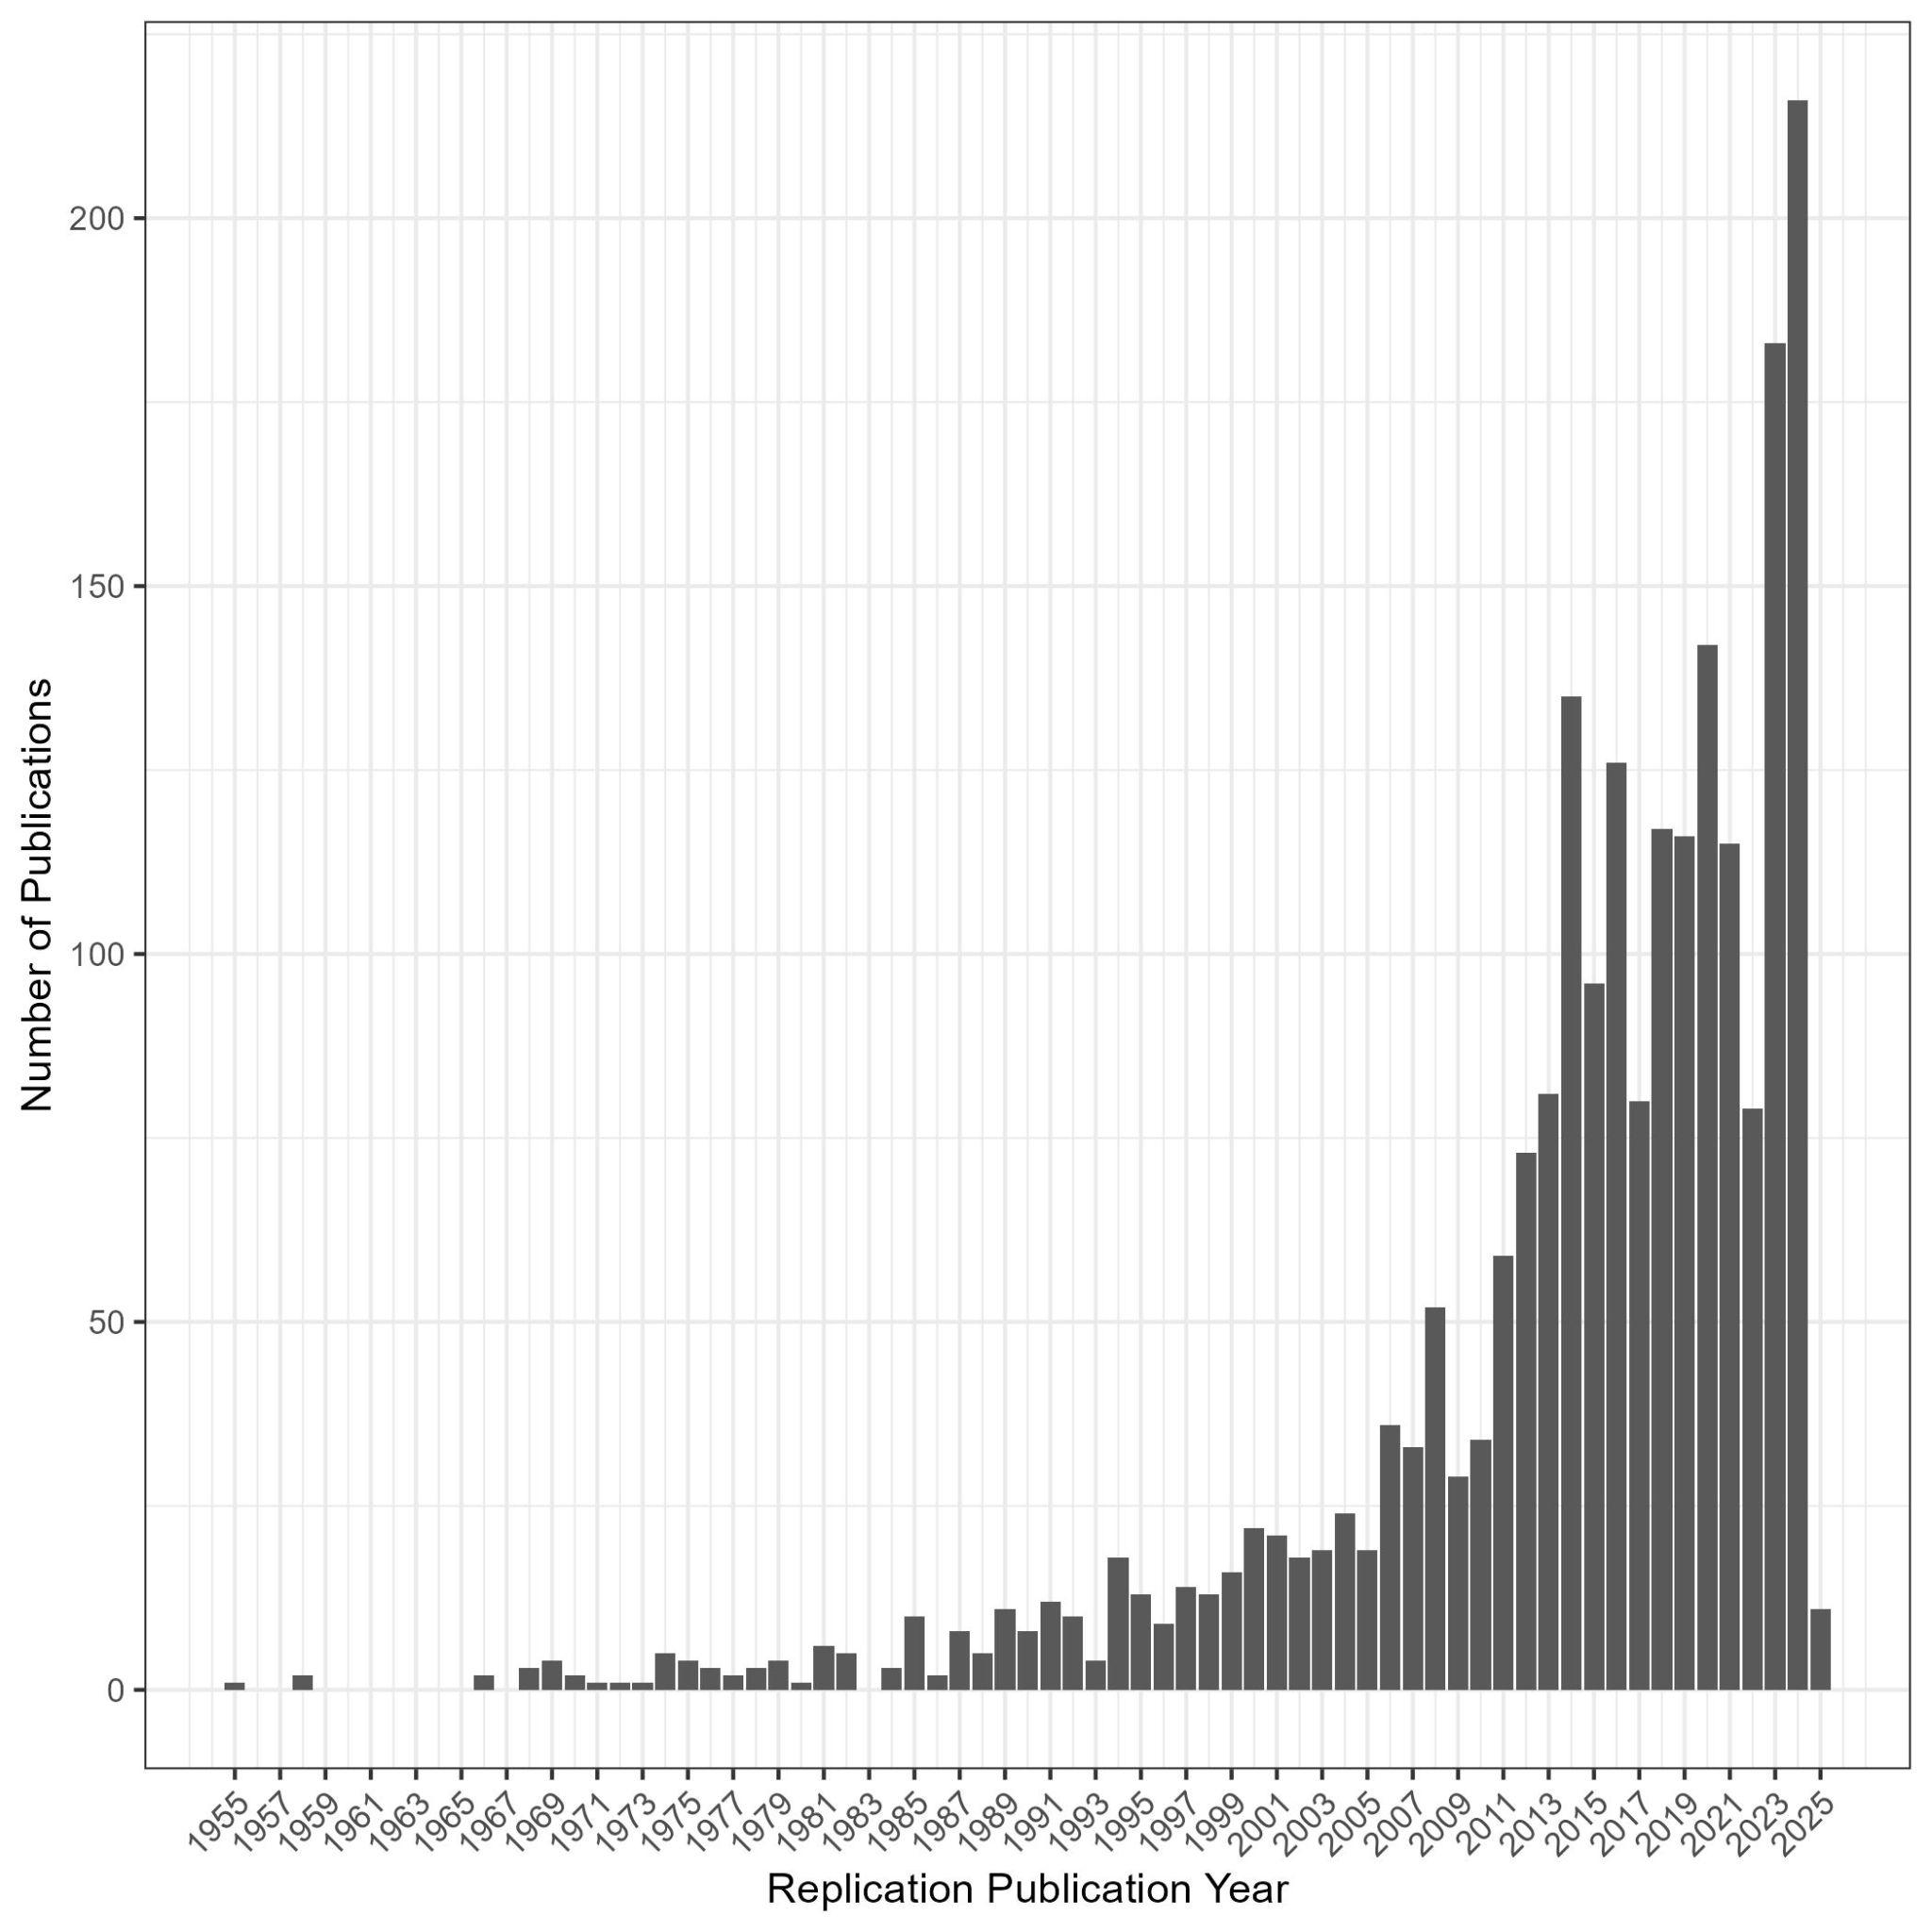
\includegraphics[keepaspectratio]{images/3Rx_Image_1.jpeg}}

}

\end{figure}%

While the number of replication and reproduction studies has increased,
the overall proportion of them is still very small, with reviews finding
yearly replication rates of up to 1\%
(\citeproc{ref-PerryEtAl2022}{Perry, Morris, and Lea 2022}). Moreover,
much of the guidance on replications is being developed actively
(\citeproc{ref-ClarkeEtAl2024}{Clarke et al. 2024}) and in narrow parts
of science, which leads to fragmentation, siloing, and potentially
inconsistent information.

Here we attempt to integrate useful guidelines (e.g.,
\citeproc{ref-BlockKuckertz2018}{Block and Kuckertz 2018};
\citeproc{ref-JekelEtAl2020}{Jekel et al. 2020}) into a comprehensive
overview that allows diverse fields to profit from each other. In sum,
this guide provides information about the entire process of research
allowing researchers at all career stages to plan, conduct, and publish
reproduction and replication studies. We limit our scope to quantitative
research, given that the concept of reproducibility and replicability
itself is highly contested among qualitative researchers (see
\citeproc{ref-MakelEtAl2012}{Makel, Plucker, and Hegarty 2012};
\citeproc{ref-ColeEtAl2024}{Cole et al. 2024};
\citeproc{ref-Pownall2022}{Pownall 2022};
\citeproc{ref-Bennett2021}{Bennett 2021}).

\chapter{Understanding Replications and
Reproductions}\label{understanding-replications-and-reproductions}

In this guide, we focus on studies that re-examine a previously tested
hypothesis and refer to them as repetitions (i.e., reproductions and
replications) with the general field being called repetitive research as
suggested by Schöch (\citeproc{ref-Schoch2023}{2023}). However, it is
important to note from the outset, that there is no overarching
terminology or consensus (e.g., \citeproc{ref-VoelklEtAl2025}{Voelkl et
al. 2025}), as the formal development of replication methods has begun
relatively late in the social, behavioral, and cognitive sciences. For
example, empirical psychology is more than 100 years old, but until the
advent of the replication/reproducibility crisis in the early 2010s,
replication methods have been rarely discussed (e.g.,
\citeproc{ref-King1995}{King 1995}). Different fields of research seem
to tackle the task differently and independently, which has led to
multiple overlapping terminologies across psychology
(\citeproc{ref-Schmidt2009}{Schmidt 2009};
\citeproc{ref-HueffmeierEtAl2016}{Hüffmeier, Mazei, and Schultze 2016}),
management (\citeproc{ref-TsangKwan1999}{Tsang and Kwan 1999}),
marketing (\citeproc{ref-UrminskyDietvorst2024}{Urminsky and Dietvorst
2024}), organizational sciences (\citeproc{ref-KohlerCortina2021}{Köhler
and Cortina 2021}), computer sciences
(\citeproc{ref-HerouxEtAl2018}{Heroux et al. 2018}), language learning
(\citeproc{ref-McManus2024}{McManus 2024}), and the humanities
(\citeproc{ref-Schoch2023}{Schöch 2023}).

\section{Reproduction and
Replication}\label{reproduction-and-replication}

The terms reproduction and replication are used in different ways
between disciplines; for example, in psychology, studies using different
data are commonly referred to as replications and studies using the same
data are referred to as reproductions, whereas in other fields, such as
computational science or economics, these terms may be used in the
opposite manner or treated interchangeably (see
\citeproc{ref-MilkowskiEtAl2018}{Miłkowski, Hensel, and Hohol 2018};
\citeproc{ref-AnkelPetersEtAl2023}{Ankel-Peters, Fiala, and Neubauer
2023}). In this paper, \emph{replication} is used to refer to efforts
involving the analysis of \emph{different data}, and \emph{reproduction}
to efforts involving the \emph{same data}. The different data do not
necessarily need to be from a different sample but can also constitute
distinct (non-overlapping) subsets from the same sample (e.g.,
incidental or panel data, \citeproc{ref-HuangHuang2024}{Huang and Huang
2024}).

Reproduction and replication should always be considered together and if
possible, \emph{reproduction should come before replication}. This is
because, at the early stages of research, reproduction is much more cost
efficient; first confirming whether the findings are reproducible can
clarify whether a replication is worthwhile. Furthermore, if the
research procedure consists of ``moving away'' from a specific finding
in terms of changing the analysis code, materials, and dataset to test
its generalizability or boundary conditions, a \emph{numerical
reproduction} (using the same data and same code) is the closest
possible repetition of a finding and a useful foundation for further
steps. We discuss multiple cases to illustrate the relationship between
reproduction and replication in Table~\ref{tbl-rep-outcomes} (Note that
a similar distinction is made by The Turing Way Community
(\citeproc{ref-TuringWay2025}{2025}) but uses a less specific
terminology for reproductions.)

\begin{longtable}[]{@{}
  >{\raggedright\arraybackslash}p{(\linewidth - 6\tabcolsep) * \real{0.2500}}
  >{\raggedright\arraybackslash}p{(\linewidth - 6\tabcolsep) * \real{0.2500}}
  >{\raggedright\arraybackslash}p{(\linewidth - 6\tabcolsep) * \real{0.2500}}
  >{\raggedright\arraybackslash}p{(\linewidth - 6\tabcolsep) * \real{0.2500}}@{}}
\caption{Possible combinations of reproduction and replication
outcomes.}\label{tbl-rep-outcomes}\tabularnewline
\toprule\noalign{}
\begin{minipage}[b]{\linewidth}\raggedright
Case
\end{minipage} & \begin{minipage}[b]{\linewidth}\raggedright
Reproducible?
\end{minipage} & \begin{minipage}[b]{\linewidth}\raggedright
Replicable?
\end{minipage} & \begin{minipage}[b]{\linewidth}\raggedright
Possible interpretation
\end{minipage} \\
\midrule\noalign{}
\endfirsthead
\toprule\noalign{}
\begin{minipage}[b]{\linewidth}\raggedright
Case
\end{minipage} & \begin{minipage}[b]{\linewidth}\raggedright
Reproducible?
\end{minipage} & \begin{minipage}[b]{\linewidth}\raggedright
Replicable?
\end{minipage} & \begin{minipage}[b]{\linewidth}\raggedright
Possible interpretation
\end{minipage} \\
\midrule\noalign{}
\endhead
\bottomrule\noalign{}
\endlastfoot
A & Yes & Yes & The original finding is reproducible and
generalizable. \\
B & Yes & No & The original finding is reproducible but not
generalizable. \\
C & No & Yes & The original finding is not reproducible but replicators
could determine a scenario where it holds. \\
D & No & No & The original finding is neither reproducible nor
generalizable. \\
\end{longtable}

\section{Outcome}\label{outcome}

Common language often conflates outcome and study descriptions:
researchers typically use the phrase ``has been replicated'' to refer to
a replication attempt that has corroborated the findings of the original
study, whereas ``failed to replicate'' or ``could not be replicated'' is
used to refer to circumstances where a replication attempt has not
corroborated the original results or has led to a different
interpretation or conclusions (see also Patil, Peng, and Leek
(\citeproc{ref-PatilEtAl2016a}{2016a})).

In this article, when we state that a ``study was
reproduced/replicated'' we mean that there has been a replication
attempt, irrespective of its outcome. With ``replicable'' and
``reproducible'' we express that there was support for the original
hypothesis. Note that the outcome of a replication/reproduction study is
often not straightforward, but may depend on the success criteria
applied. This is discussed in Section~\ref{sec-success-criteria}.

\section{Types of replication}\label{types-of-replication}

We heavily rely on the typology provided by Hüffmeier, Mazei, and
Schultze (\citeproc{ref-HueffmeierEtAl2016}{2016}) where different types
of replications are defined by the \emph{closeness} or \emph{similarity}
between original and replication study. Similarity cannot be evaluated
without a theory about the concepts involved. For example, the concept
of age can differ strongly between replications of historical,
psychological, or biological studies, leading to different measures of
the concept itself and thus different judgments about the similarity of
an object's age.

Under the assumption of a stable world and constant laws or regularities
that are investigated by the social, behavioral, and cognitive sciences,
a reproduction and replication study's closeness to an original study is
associated with replication `success'
(\citeproc{ref-sec-success-criteria}{\textbf{sec-success-criteria?}}).
The argument can be made from two different philosophical perspectives
that we call inductive (phenomenon-focused, effects application,
bottom-up) and deductive (theory-focused, theory application, top down,
e.g., \citeproc{ref-CalderEtAl1981}{Calder, Phillips, and Tybout 1981};
\citeproc{ref-BorgstedeScholz2021}{Borgstede and Scholz 2021}). From an
inductive perspective, a replication that is very similar to an original
study should lead to the same result whereas one that differs with
respect to any criterion may lead to different results.\footnote{From an
  extreme inductive perspective that stresses that there is no logical
  foundation in inferring future events from previous events (Hume,
  1748/2016), one could even argue that it may not make a difference
  whether one tries to make the same observation again under the same or
  different circumstances.} This is a stance often taken by proponents
of findings that failed to replicate (e.g.,
\citeproc{ref-BaumeisterVohs2016}{Baumeister and Vohs 2016};
\citeproc{ref-Syed2023}{Syed 2023}), arguing that characteristics such
as time or place are different and can be valid reasons for different
results. From a deductive (theory-focused) view, the only changes that
matter are those that affect the underlying theory. Consider for example
a replication experiment that is identical in every aspect except for
the season (summer instead of winter). If the theory that is tested is
about color perception, the replication is likely judged to be close to
the original study but if it is about participants' current tea
preferences, it is likely judged to be different from the original study
in a theoretically relevant aspect.\footnote{On a different note, Vohs
  et al.~(2021) published a study that was different from previous
  studies in that it did not replicate any previous study but was
  instead designed to be ideal to test the theory and estimate the
  average effect size and termed it ``paradigmatic replication
  approach''. Given the present terminology, we do not consider this a
  replication.} A related dimension of closeness concerns
\emph{contextual sensitivity}---the extent to which the meaning of a
questionnaire or the effect of a manipulation depends on time, culture,
or population. As Van Bavel et al.
(\citeproc{ref-VanBavelEtAl2016}{2016}) demonstrate, studies on
contextually sensitive topics were significantly less likely to
replicate successfully in Open Science Collaboration
(\citeproc{ref-OpenScienceCollab2015}{2015}), even though methodological
fidelity was high. This raises important questions about what
constitutes a ``close'' replication: Should a study on celebrity
attitudes, for example, use the same examples (which may be outdated and
thus psychologically inert), or should it adapt to locally and
temporarily salient figures to trigger the same cognitive or emotional
responses? In such cases, strict methodological similarity might
paradoxically undermine theoretical closeness, and thus the validity of
the replication attempt. This tension highlights that \emph{procedural}
fidelity does not always equate to \emph{theoretical}
equivalence---particularly for studies involving social meaning,
identity, or temporally anchored norms. LeBel et al.
(\citeproc{ref-LeBelEtAl2018}{2018a}) provide a taxonomy for classifying
a replication study's closeness for psychological research.

\begin{figure}

\caption{\label{fig-taxonomy-similarity}Taxonomy for classifying a
replication study's methodological similarity to an original study.
\emph{Reprinted from LeBel et al.
(\citeproc{ref-LeBelEtAl2018fig}{2018b}) with permission.}}

\centering{

\pandocbounded{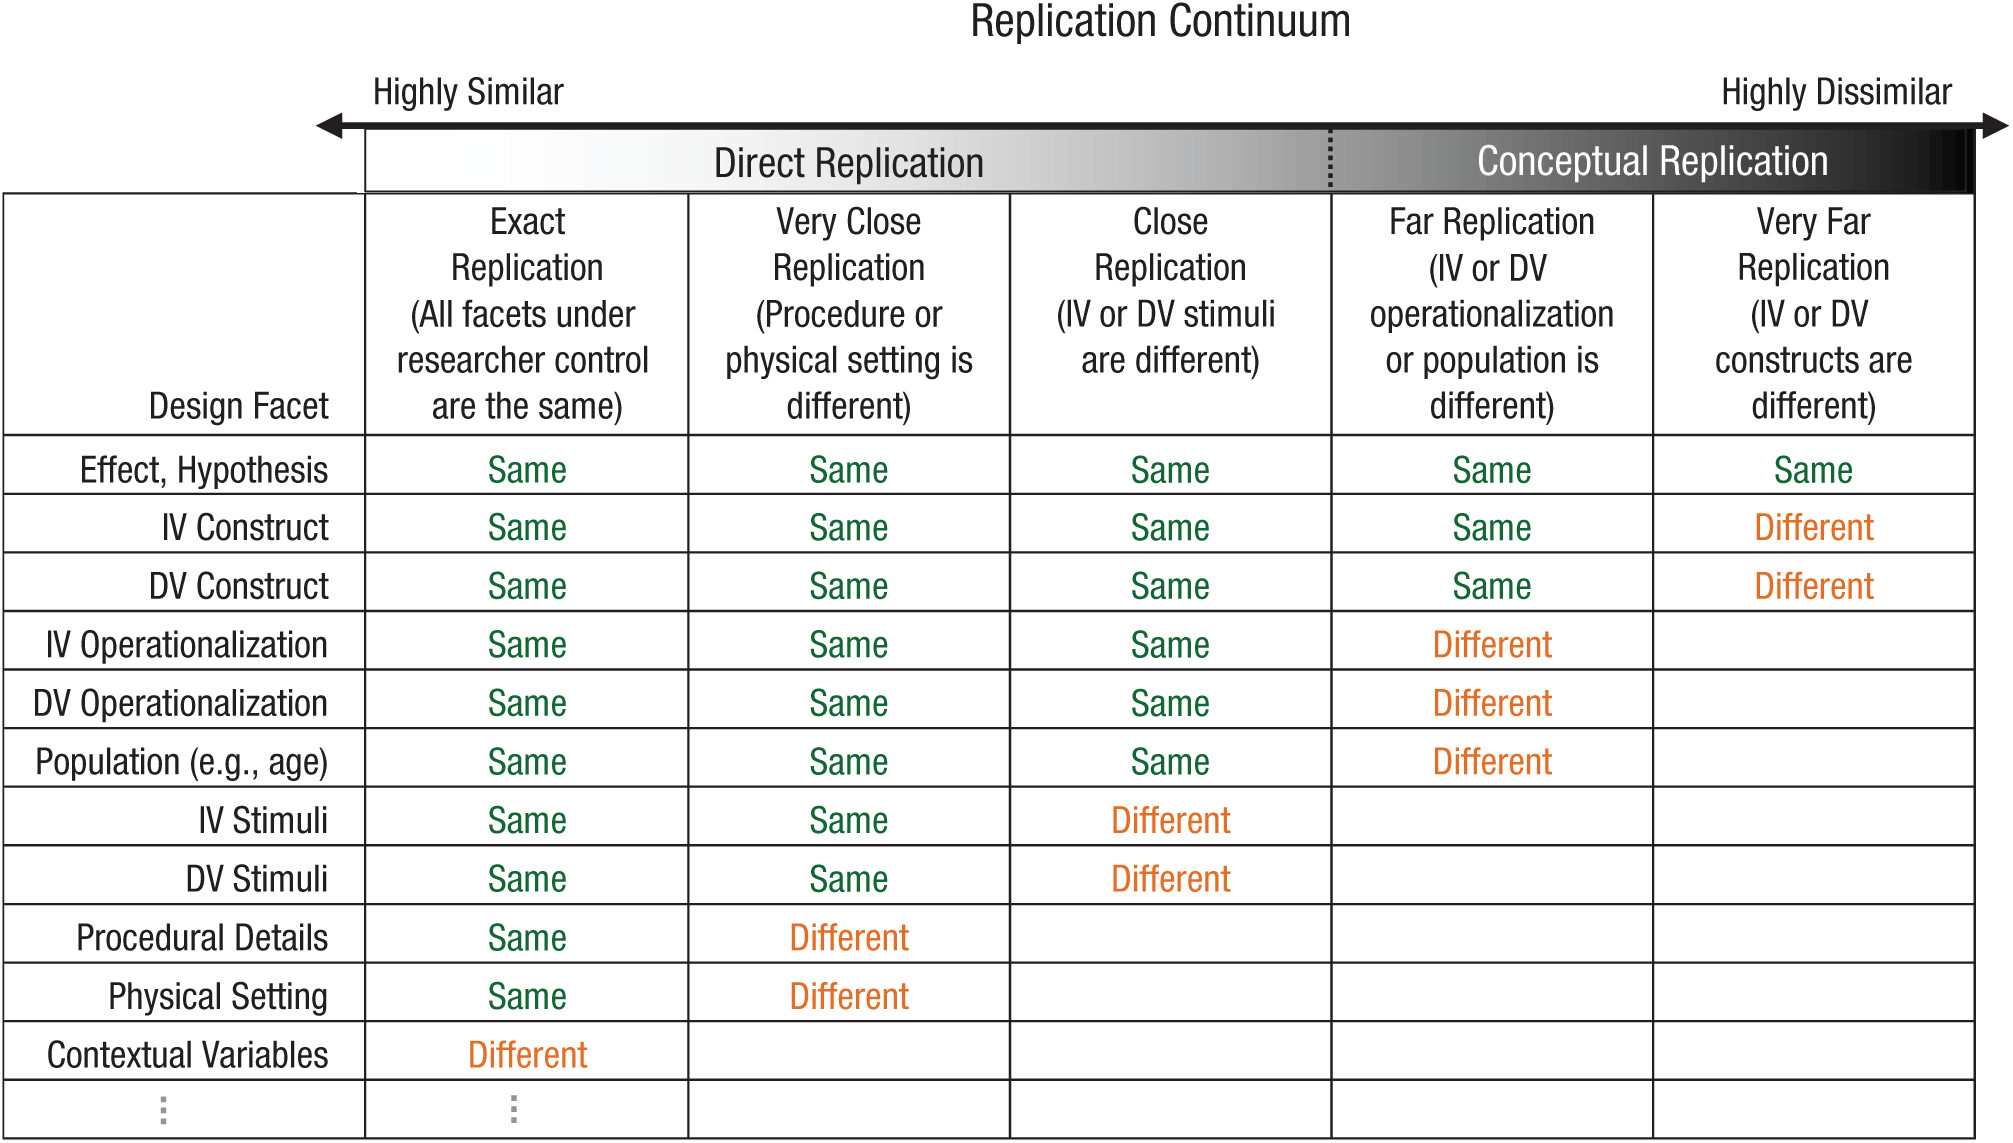
\includegraphics[keepaspectratio]{images/sTS_Image_2.png}}

}

\end{figure}%

Support for the view that methodological features that are theoretically
irrelevant such as the use of text versus image stimuli or the type of
sample can have a strong impact on the results is provided by Landy et
al. (\citeproc{ref-LandyEtAl2020}{2020}), who let different groups of
researchers test identical hypotheses using different study designs. The
groups arrived at entirely different and even opposite conclusions for
similar hypotheses. The differences in the study designs were not
predicted by the theories involved in the respective studies: A priori,
none of the differences (e.g., within- vs.~between-subjects design,
picture vs.~text stimuli) ``should'' have affected the conclusions. Note
that other theories such as demand characteristics
(\citeproc{ref-orne2017social}{Orne 2017}) could help in these cases.
Moreover, this does not disconfirm the deductive perspective but may be
a demonstration of the lack of specification of theories - as well as a
reminder that statistical choices affect statistical power by changing
the variance, and thus standardised effect sizes. In line with
deviations from original studies mostly having uncertain consequences,
close replications more directly test the credibility of original
results, while conceptual replications that vary features of the design
are concerned with generalizability.

Note that Nosek and Errington (\citeproc{ref-NosekErrington2020}{2020})
define replication as a study ``for which any outcome would be
considered diagnostic evidence about a claim from prior research''. This
can lead to issues when the original claim is not clear on its boundary
conditions. Conceptual replications that highlight limitations to the
claim made clearly count, e.g.~when the original claim was about a
universal effect, and the replication shows that it does not hold in a
specific country. Conversely, ``replications'' that go beyond the claim
made, and test the transferability of a claim explicitly made about,
e.g., maths education to science education may indeed serve to be framed
differently, as they do not directly speak to the claim made originally.
Where original authors' failed to specify the scope of their claim, we
would understand that they imply a broad/universally applicable
relationship, which any attempts at generalisation help to corroborate
or specify.

In terms of Schöch (\citeproc{ref-Schoch2023}{2023}), who defines an
overarching type of \emph{repetitive research} based on multiple
dimensions, replications are concerned with the same question as a
previous study, use the same (close replication) or a similar
(conceptual replication) method and use different data (otherwise they
are reproductions).

\section{Types of reproduction}\label{types-of-reproduction}

Reproductions can be numerical reproductions, testing whether the same
data, code and software lead to the same results, or robustness
reproductions, extending the original analysis and exploring the central
finding's limits (Dreber and Johannesson
(\citeproc{ref-DreberJohannesson2024}{2024})). Most reproductions would
include both a numerical reproduction as baseline and then a robustness
reproduction, unless the numerical reproduction is not possible due to a
lack of code or software.

\part{The Replication Process}

\chapter{Choosing the Target Study}\label{choosing-the-target-study}

Reproduction and replication studies can serve different goals and
depending on the goal, the way of choosing a target study differs (see
\citeproc{ref-PittelkowEtAl2023}{Pittelkow et al. 2023}). In large-scale
reproduction and replication projects, such as Brodeur et al.
(\citeproc{ref-BrodeurEtAl2024b}{2024}), the Reproducibility Project:
Psychology (\citeproc{ref-OpenScienceCollab2015}{Open Science
Collaboration 2015}) or the Reproducibility Project: Cancer Biology
(\citeproc{ref-ErringtonEtAl2021b}{Errington, Mathur, et al. 2021}), the
primary aim is to assess the overall reliability of a field or a set of
findings, leading to a top-down approach in which the decision to
replicate comes first, followed by the selection of specific replication
targets. This is often done in a way aimed to be representative of a
field, ideally through random sampling, though this is generally
constrained by practicalities. Here, individual studies are not the
primary focus in the decision to repeat; instead, choices are guided by
broader methodological or theoretical considerations. In contrast,
individual researchers frequently adopt a bottom-up approach, where the
decision to replicate is driven by engagement with a specific study (or
theoretically related set of studies, e.g.,
\citeproc{ref-RoselerEtAl2021}{Röseler et al. 2021}). This may occur
when a researcher wishes to build upon an existing finding and seeks to
verify its robustness before doing so, or when they harbor doubts about
a claim and aim to test its validity. Since reproductions and
replications can serve multiple purposes---from assessing theoretical
frameworks to correcting potential errors---there is no singular correct
way to decide what to repeat. The choice of targets ultimately depends
on the overarching goals and methodological approach of the replication
effort, as well as on practical constraints. However, what does matter
is that the selection of reproduction and replication targets is well
justified and transparently communicated. For instance, researchers can
use structured frameworks such as the replication target selection
checklist to ensure clarity and consistency in their decision-making
process (\citeproc{ref-PittelkowEtAl2023}{Pittelkow et al. 2023}). For a
comment on what empirical reasons for replications are, see Kamermans et
al. (\citeproc{ref-KamermansEtAl2025}{2025}).

\section{Determining Reproduction and Replication
Value}\label{determining-reproduction-and-replication-value}

Whether a target study is ``worth reproducing'' or ``worth replicating''
is highly debated and is suggested to depend on several overlapping
factors, including value (sometimes also referred to as impact or
relevance), uncertainty, and feasibility
(\citeproc{ref-IsagerEtAl2023}{P. M. Isager et al. 2023}). Below,
different suggestions for operationalizing these factors are discussed
systematically.

Note that there is also ongoing discussion about whether or not all
studies are generally `worth replicating'. One perspective is \emph{what
is worthy of publication is worthy of replication}
(\citeproc{ref-Feldman2025}{Feldman 2025}) or on a different note, what
is worthy of publication \emph{should be }worthy of replication - though
this perspective is becoming complicated through the rise of influential
preprints and a public-review-curate model to publications. Naturally, a
public report of a study is necessary for other researchers to attempt a
replication and an available dataset is needed for a reproduction. To
take a more fine-grained look at the publication status, several
different types of research emerge. An article can be \emph{retracted},
that is, there is no confidence anymore in its findings due to research
misconduct or severe errors. When the data of a study were fabricated
and it was thus retracted, a reproduction will not be informative but a
replication may inform researchers about the correctness of the
hypothesis unlike the original report. Other reasons (or unclear
reasons) for retraction may conversely increase the replication and
reproduction value, as the source of a true claim may have become
untrustworthy (and not easily citeable) due to issues unrelated to its
truth (e.g.~plagiarism).

Replicating and reproducing every finding that was ever published
appears impossible to achieve, which is why researchers need to make
decisions about prioritization. In the following, we discuss criteria by
which such a prioritization can occur - restricted to quantitative
research.

\section{Value}\label{value}

The original study should be somehow relevant for the replication to
have value (e.g., \citeproc{ref-KarhulahtiEtAl2024}{Karhulahti,
Martončik, and Adamkovic 2024}). It may have started a research stream.
For example, Jacowitz and Kahneman's
(\citeproc{ref-JacowitzKahneman1995}{1995}) studies on anchoring and
adjustment were fundamental for how anchoring effects are investigated
today, and were therefore replicated by Klein et al.
(\citeproc{ref-KleinEtAl2014}{2014}). Field et al.
(\citeproc{ref-FieldEtAl2019}{2019}) propose a method for the selection
of replication studies that features the theoretical importance of the
original study result. Relevance may be evidenced by many citations as
they show that many studies are building on the finding, testing similar
hypotheses, or criticizing the study. Note that a study could also be
cited as a negative example or study that has not been replicated or
retracted for some reason. Isager et al.
(\citeproc{ref-IsagerEtAl2023}{2023}) suggest deciding what to replicate
based on sample size and citation count (but see
\citeproc{ref-PittelkowEtAl2025}{Pittelkow, Field, and Ravenzwaaij
2025}). In a Delphi study examining consensus among psychologists that
had conducted empirical replications on what should influence the
decision of what study to replicate, elements that came up were the
importance of the original study for research (as indicated by
citations, the phenomenon being over- or understudied, and the impact
factor of the journal), the theoretical relevance of the study, and the
implications of the original study for practice, policy, or clinical
work (\citeproc{ref-PittelkowEtAl2023}{Pittelkow et al. 2023}). The
relevance of societal impact was also stressed by
(\citeproc{ref-Bekkers2024}{2024}), as a study may have a high value for
a societal problem (e.g., a new vaccine or a repeated test of a claim
that is relevant in the political discourse such as criminality among
immigrants).

For scientists reproducing or replicating a study because they are
interested in building on its findings (including if they wish to build
upon their own original findings), their interest to build on it may be
a sufficient indicator of its relevance to their research program.

\section{Uncertainty}\label{uncertainty}

The more uncertain the original study's outcome is, the higher the
potential of knowledge gained from reproduction and replication.
Although no findings are definitive, research reports differ in the
strength of the evidence they present (e.g., Registered
Reports\footnote{For registered reports, a journal reviews only the
  introduction and method and no data have been collected at this point
  of time. After an initial revision and ``in-principle acceptance,''
  results are collected and the full report submitted. The second round
  of review is concerned only with the authors' adherence to the
  preregistration and success to execute the planned study.} are
typically more convincing than non preregistered studies,
\citeproc{ref-SoderbergEtAl2021}{Soderberg et al. 2021}). Similarly,
sample size (within a given field) has been proposed as an indicator of
evidence strength (\citeproc{ref-IsagerEtAl2021}{Peder Mortvedt Isager
et al. 2021}). Pittelkow et al.
(\citeproc{ref-PittelkowEtAl2021}{2021}), Pittelkow et al.
(\citeproc{ref-PittelkowEtAl2023}{2023}) and Field et al.
(\citeproc{ref-FieldEtAl2019}{2019}) all argued for using the current
strength of evidence in favour of the original claim as an important
element that features into the choosing a replication target. However,
the degree of uncertainty can be uncertain or misjudged: In some areas
of research a hypothesis had been claimed to be confirmed hundreds of
times and yet, large-scale replication effort could not support the
original hypothesis so that after hundreds of studies the existence of
the phenomenon was still unknown (e.g.,
\citeproc{ref-FrieseEtAl2019}{Friese et al. 2019}). Meta-analyses allow
some tests for uncertainty (e.g.~via correction of bias, evaluation of
risk of bias, or estimates of heterogeneity). Although there are
numerous ways to meta-analytically evaluate the expected replicability
of a set of claims, none of them is as solid as a well-designed
replication attempt (\citeproc{ref-CarterEtAl2019}{Carter et al. 2019}).
Other heuristics to estimate robustness reproducibility and
replicability of sets of findings have been proposed:. They include the
caliper test, relative proximity, or \emph{z}-curve
(\citeproc{ref-BartosSchimmack2022}{Bartoš and Schimmack 2022}; see
\citeproc{ref-AdlerEtAl2023}{Adler, Röseler, and Schöniger 2023}, for an
overview and a ShinyApp that combines these tools). Individual findings
can be assessed through forensic meta-science tests (for an overview,
see \citeproc{ref-Heathers2025}{Heathers 2025}), and through the
assessment of papers for reporting issues, such as those identified by
\emph{statcheck} (\citeproc{ref-NuijtenPolanin2020}{Nuijten and Polanin
2020}; \citeproc{ref-papercheckR}{DeBruine and Lakens 2025}). Moreover,
methods such as \emph{sum of p-values}
(\citeproc{ref-HeldEtAl2024}{Held, Pawel, and Micheloud 2024}) and
Bayesian re-analysis can be applied to help determine the degree of
evidence for a given effect an original study might contain
(\citeproc{ref-FieldEtAl2019}{Field et al. 2019};
\citeproc{ref-PittelkowEtAl2021}{Pittelkow et al. 2021}).

If the original paper reports multiple studies for the same phenomenon,
researchers should check the proportion of significant studies and
whether all of them confirm the hypothesis. More studies reduce the
overall statistical power (power deflation). Provided the hypothesis is
correct, a single study may test it with 90\% power, that is, the
statistical analysis will indicate the correctness of the hypothesis
with a probability of .9. Now, if 10 studies are run with 90\% power
each, the chances of all of them supporting the hypothesis (even if it
is true) are \(0.9^{10} \approx 0.35\). For 80\%, even finding five
significant findings in a row is fairly unlikely
(\(0.8^{5} \approx 0.33\)). Thus, studies reporting a set of many and
only significant findings when each of the studies does not have very
high power should be taken with caution (see also
\citeproc{ref-Francis2012}{Francis 2012};
\citeproc{ref-Schimmack2012}{Schimmack 2012};
\citeproc{ref-LakensEtz2017}{Lakens and Etz 2017}).

For large parts of the literature and given the overall low
replicability rate in many fields (though not all, e.g.,
\citeproc{ref-Soto2019}{Soto 2019}), the mere lack of a reproduction or
close replication by independent researchers can be used as an argument
for uncertainty (e.g., \citeproc{ref-PittelkowEtAl2023}{Pittelkow et al.
2023}). If a study has only been replicated by the original authors, it
can be indicative of nobody else being interested in the phenomenon
(i.e., low replication value) or nobody else being able to provide
evidence for it (i.e., high uncertainty). For example, it is possible
that reports of failed replications are held back by reviewers due to an
aversion to null findings, replications, or findings criticizing their
own work.

As replications can also be used to probe a phenomenon's
generalizability, a lack of variety in study designs can motivate a
replication attempt. If there is reason to assume that a phenomenon is
highly dependent on context (e.g., works only for graduate students,
with English-speaking people, when people are incentivized, for the
chosen stimuli, \ldots), it can be replicated and extended in other
contexts. More generally, when background factors are introduced to a
study (e.g., there was a positive correlation in study X but researchers
suspect it to vanish under condition M), the original finding needs to
be replicated in a part of the new study for the argument to work. An
added benefit of this is to help avoid later claims of `hidden
moderators' in original studies; an argument which has been used
previously to refute the validity of replication study results
(\citeproc{ref-ZwaanEtAl2018}{Zwaan et al. 2018}).

Finally, uncertainty can be the result of a lack of specificity in the
original report: If there are details missing that cannot be retrieved
anymore (e.g., researchers involved in the original study cannot be
reached), a replication can develop, test and share a comprehensive set
of materials. For example, Chartrand and Bargh's
(\citeproc{ref-ChartrandBargh1999}{1999}) seminal study on the
\emph{chameleon effect} requires many materials but none of them are
openly available. Accordingly, Pittelkow et al.
(\citeproc{ref-PittelkowEtAl2023}{2023}) identified the clarity of the
original study protocol as an important element that features into the
decision of replication study selection. Reconstructing these materials
and documenting a procedure would, thus, be a valuable contribution of a
replication study.

\textbf{\emph{Theoretical contribution}}

In some cases, theories are so vague that a failed replication would
likely be criticized for misunderstanding the theory (e.g.,
\citeproc{ref-BaumeisterVohs2016}{Baumeister and Vohs 2016}). This
suggests that the target theory was not well specified. If accepted as a
reason not to replicate, it can discourage any form of replication
despite the target finding being relevant. Instead, replication
researchers can ask original authors for feedback on the study protocol
before collecting data to try to ensure that it tests (and then
articulates) the intended theory. They can also engage in adversarial
collaboration or ``red teaming'' (e.g.,
\citeproc{ref-CowanEtAl2020}{Cowan et al. 2020};
\citeproc{ref-ClarkEtAl2022}{Clark et al. 2022};
\citeproc{ref-CorcoranEtAl2023}{Corcoran, Hohwy, and Friston 2023}),
that is work together with the original authors to design a study that
they agree would be able to corroborate the original claim, or to call
it into doubt.

Nevertheless, it has been argued that because so many original studies
are flawed, the theories built upon them are weak, or contaminated.
This, in turn, can lead to flawed replication studies, especially in the
case of theory that aims to explain phenomena
(\citeproc{ref-FieldEtAl2024}{Field et al. 2024}), risking a vicious
cycle in which successful replications potentially perpetuate flaws
across studies.

\textbf{\emph{Availability of reproductions and replications}}

While a single replication (or robustness reproduction) cannot provide
conclusive evidence in regard to the veracity of original claims, the
first numerical reproduction, and arguably also the first robustness
reproduction and replication adds the greatest value in terms of
reducing uncertainty. Therefore, the search for existing reproductions
and replications is a key part of the selection of a target study.

Although there is no comprehensive database with reproductions yet,
researchers can check resources such as the Institute for Replication's
discussion paper series
(\url{https://i4replication.org/discussion_paper.html}, c.f.
\citeproc{ref-BrodeurEtAl2024b}{Brodeur, Dreber, et al. 2024}), the
ReplicationWiki (\citeproc{ref-Hoeffler2017}{Höffler 2017}), the
CODECHECK register (\url{https://codecheck.org.uk/register/}, c.f.
\citeproc{ref-NuestEglen2021}{Nüst and Eglen 2021}), or the Social
Science Reproduction Platform
(\url{https://www.socialsciencereproduction.org}).

With regard to replications, researchers can browse the FORRT
Replication Database
(\url{https://forrt-replications.shinyapps.io/fred_explorer/}, c.f.
\citeproc{ref-RoselerEtAl2024}{Röseler et al. 2024}), though this does
not (yet) provide a replacement for manual searches.

\section{(Potential) Researcher Bias}\label{potential-researcher-bias}

Researchers typically work in relatively small communities to
investigate the same phenomenon. These researchers are invested in their
work and can be influenced by certain researcher biases, such as
confirmation bias (the tendency to preferentially seek out, evaluate and
recall information that supports one's existing beliefs, see
\citeproc{ref-Mahoney1977}{Mahoney 1977}) and motivated reasoning
(generating post-hoc rationalizations that frame previous decisions in a
favourable light, see \citeproc{ref-HardwickeWagenmakers2023}{Hardwicke
and Wagenmakers 2023}; \citeproc{ref-MunafoEtAl2020}{Munafò et al.
2020}). In some cases, researchers profit off their work and the
(perceived) replicability of their findings may be associated with
personal financial gain. Such conflicts of interest should be disclosed,
but this is not always the case (see
\citeproc{ref-HeireneEtAl2024}{Heirene et al. 2024}).

However, replication researchers are just as prone to bias as original
authors can be. Certain studies are more likely to be chosen for
replication than others (see \citeproc{ref-Pennington2023}{Pennington
2023}; \citeproc{ref-Yarkoni2013}{Yarkoni 2013}), and there \emph{may}
be a publication bias in replication studies in favor of nonsignificant
findings (\citeproc{ref-BerinskyEtAl2021}{Berinsky, Druckman, and
Yamamoto 2021}), though there is no empirical evidence for this yet.
Nevertheless, greater interest in failed replications seems very likely,
incentivizing replication researchers to apply questionable research
practices (QRPs) so that the results are nonsignificant (``null
hacking,'' \citeproc{ref-Protzko2018}{Protzko 2018};
\citeproc{ref-BaumeisterEtAl2022}{Baumeister, Tice, and Bushman 2022}).
The problems of \emph{p}-hacking and null-hacking can mostly be solved
through preregistration and the use of Registered (Replication) Reports
(e.g., \citeproc{ref-BrodeurEtAl2024b}{Brodeur, Dreber, et al. 2024};
\citeproc{ref-SoderbergEtAl2021}{Soderberg et al. 2021}). Another type
of bias is that researchers may be interested in replicating specific
studies because of personal admiration towards a study or envy towards a
colleague.

\section{Feasibility}\label{feasibility}

Reproductions require the original dataset. We recommend that
researchers check whether the journal that published the original study
has a data editor or reproducibility manager who has done a
reproducibility check or provides a \emph{replication package}. A
replication package is a collection of materials to allow reproduction
of the original results. Ideally, the dataset in the replication
package, or shared separately, adheres to the FAIR criteria
(\citeproc{ref-WilkinsonEtAl2016}{Wilkinson et al. 2016}), that is, it
should be findable, accessible, interoperable, and reusable. Otherwise,
the reproduction author would need to send a data sharing request to the
original authors. In any case, they may need to consult with the
original authors regarding software versions and code that does not work
anymore due to changes in the software.

While original data is not necessary for replications, thorough
documentation of the original study is highly beneficial. Moreover,
replication researchers should evaluate whether they can achieve the
target sample size, which is often a multiple of the original sample
size (see section \hyperref[heading=h.r1a225ca00xn]{Sample Size
Determination}). Pittelkow et al.
(\citeproc{ref-PittelkowEtAl2023}{2023}) identified the resources
available to the replicating team in terms of funding, time, equipment,
and (if relevant) previous experience and expertise as important
elements that feature into the replication study selection. When
choosing a target study, researchers should try to anticipate practical
problems, and should restrict their choice of replication target to
align with their lab resources in order to prevent `secondary' research
waste (\citeproc{ref-FieldEtAl2019}{Field et al. 2019}). Specifically,
some studies may be difficult to replicate (e.g., longitudinal studies).
Other studies, such as those conducted with the use of highly technical,
restricted, or expensive equipment, such as studies involving MRI
scanning, might require expertise and knowledge that is not represented
in all potential replication research teams
(\citeproc{ref-FieldEtAl2019}{Field et al. 2019}).

Moreover, there are no established standards for replications in some
fields yet. In that case, replications may add less to the reduction of
uncertainty and replicators need to propose methods. For example,
replications with response-surface-analyses are not as established as
those with \emph{t}-tests for two-group study designs. Furthermore, the
complexity of the data types can pose challenges for definitions of
successful replications, such as in neuroimaging research (e.g., MRI
studies) which often implicates outcome variables with an additional
spatial component.

\chapter{Planning and Conducting Reproductions and
Replications}\label{planning-and-conducting-reproductions-and-replications}

Planning depends on whether the focus is on a certain method or a
theory, that is whether the replication will be close or conceptual.
Table~\ref{tbl-rep-types} provides an overview of reproduction and
replication types, or more generally ``repetitive research''
(\citeproc{ref-Schoch2023}{Schöch 2023}), drawn from different resources
(e.g., \citeproc{ref-DreberJohannesson2024}{Dreber and Johannesson
2024}; \citeproc{ref-HueffmeierEtAl2016}{Hüffmeier, Mazei, and Schultze
2016}; \citeproc{ref-CortinaEtAl2023}{Cortina, Köhler, and Aulisi
2023}). The decision between these types is the first step in planning.

In addition, the formation of the replication team is important, as
replications can take substantial resources. Notably, repetitive
research has successfully been conducted collaboratively with graduate
and undergraduate students (e.g., \citeproc{ref-BoyceEtAl2024}{Boyce et
al. 2024}; \citeproc{ref-HawkinsEtAl2018}{Hawkins et al. 2018};
\citeproc{ref-JekelEtAl2020}{Jekel et al. 2020};
\citeproc{ref-MoreauWiebels2023}{Moreau and Wiebels 2023}) and we
recommend the use of replication studies to engage students of different
levels in conducting and publishing research.

\begin{longtable}[]{@{}
  >{\raggedright\arraybackslash}p{(\linewidth - 4\tabcolsep) * \real{0.3333}}
  >{\raggedright\arraybackslash}p{(\linewidth - 4\tabcolsep) * \real{0.3333}}
  >{\raggedright\arraybackslash}p{(\linewidth - 4\tabcolsep) * \real{0.3333}}@{}}
\caption{Types of repetitive research ordered by reproduction and
replication and respective closeness to the original
study.}\label{tbl-rep-types}\tabularnewline
\toprule\noalign{}
\begin{minipage}[b]{\linewidth}\raggedright
Type
\end{minipage} & \begin{minipage}[b]{\linewidth}\raggedright
Description
\end{minipage} & \begin{minipage}[b]{\linewidth}\raggedright
Goals
\end{minipage} \\
\midrule\noalign{}
\endfirsthead
\toprule\noalign{}
\begin{minipage}[b]{\linewidth}\raggedright
Type
\end{minipage} & \begin{minipage}[b]{\linewidth}\raggedright
Description
\end{minipage} & \begin{minipage}[b]{\linewidth}\raggedright
Goals
\end{minipage} \\
\midrule\noalign{}
\endhead
\bottomrule\noalign{}
\endlastfoot
Computational Reproduction & Reanalysis of the same data with the same
code & Correctness of original report \\
Recoding reproduction & Reanalysis of the same data, with new
(equivalent) code & Correctness of original report \\
Robustness Reproduction & Reanalysis of the same data with new coding
choices; can vary in closeness & Robustness of original finding and
sensitivity to different analytical decisions or software \\
Multiverse analysis & Analyze data in all sensible ways (i.e., a large
number of different robustness reproductions) & Robustness and
generalizability of original finding, identification of potential
moderators or sources for effect variability \\
Internal replication & Replicate one of your own studies as closely as
possible & Demonstrate one's findings' generalizability across studies
and rule out fear of false-positives (e.g., for new discoveries) \\
Close / direct / exact replication & Conduct a new study (based on work
by other researchers) that is as close as possible to the original study
& Rule out fear of the original finding being a false-positive, validate
original materials or design, check generalizability/external validity
for theoretically irrelevant variables (e.g., population, year of data
collection) \\
Close replication with extension & Add a variable or procedure to a
close replication & Rule out fear of the original finding being a
false-positive, test generalizability of original finding \\
Conceptual / constructive replication & Conduct a study with changes
that may be theoretically relevant but that tests the same hypothesis
(e.g., different operationalization) & Generalizability of original
finding, validity of theory \\
\end{longtable}

\section{Post Publication
Conversations}\label{post-publication-conversations}

When planning the replication study, additional knowledge should be
taken into account such as any discussions of the original finding.
There can be other studies citing the original studies, criticizing
them, disconfirming their underlying theory, identifying errors,
reinterpreting the finding, or making suggestions for replications. All
of these might highlight considerations that need to be taken into
account when designing a replication study that \emph{robustly }tests
the original claim or its generalisability.

Thus, replication researchers should look for post-publication
discussions on the target study such as published comments and reviews,
blog posts, or discussions on social media. These can often be found via
Altmetric (\url{https://www.altmetric.com}) or other tools that allow
researchers to quickly identify discussions on social media or news
outlets beyond scientific journals (\href{https://pubpeer.com}{PubPeer},
\href{https://web.hypothes.is}{Hypothes.is}, or the in-development
platform \href{https://www.alphaxiv.org/}{Alphaxiv.org}; for a review
see Henriques et al. (\citeproc{ref-HenriquesEtAl2023}{2023})).

\section{Reproduction before
Replication}\label{reproduction-before-replication}

Many features of a replication study rest on the correctness of the
original report. A reproduction allows researchers to investigate this
by being able to uncover coding errors, fraud, robustness to analytical
decisions, and generalizability. To make efficient use of resources, we
encourage researchers to investigate the original finding's
reproducibility and robustness first. In other words, ideally,
reproductions should take place before planning and conducting a
replication study. Depending on the availability of the code and data,
these can take several minutes to weeks.

If the original code and dataset are available, researchers can try to
\emph{numerically reproduce} the results. Beware, however, that
differences in software versions or default settings may lead to slight
deviations or require corrections in some cases (for a large-scale test
of reproducibility see \citeproc{ref-BrodeurEtAl2024b}{Brodeur, Dreber,
et al. 2024}). Similarly, the lack of a set seed for random number
generators can mean that analyses relying on random numbers (e.g.,
bootstrapping) cannot be exactly reproduced. If no analysis script is
available, analyses need to be recreated from the descriptions in the
report (\emph{recoding reproduction}). In this case, special attention
should be paid to processing steps such as exclusion of outliers,
transformation of variables, and handling of missing data. However, in
many research areas information on these steps is often incomplete
(\citeproc{ref-FieldEtAl2019}{Field et al. 2019}); older research tends
to be especially limited in terms of the methodological details they
provide. In addition, we recommend testing the robustness of the
original finding by making small alterations to the data processing and
analyses procedure (\emph{robustness reproductions}). For example, if
the analyses were run for a subset of the data (e.g., participants aged
21 to 30 or without outliers ± 3 standard deviations), this subset can
be changed (e.g., participants aged 18 to 30 or without outliers ± 2
standard deviations). Here, the initial focus should be on choices that
are not determined by the \emph{theory }that is presented, though this
can also be used to explore the generalisability of some aspects of
theory. Finally, if the original study was preregistered and the
original code is available, reproduction researchers can check whether
the original analyses adhere to the preregistered analysis plan.

If neither code nor data are available (or shared by the authors), no
reproduction is possible. Researchers can still use automated tools to
compare reported \emph{p}-values with those that can be computed from
test statistics via the website statcheck.io (where documents may be
uploaded), the corresponding R package
(\citeproc{ref-NuijtenPolanin2020}{Nuijten and Polanin 2020}), or
papercheck (\citeproc{ref-papercheckR}{DeBruine and Lakens 2025}), which
is still actively maintained.

\begin{figure}

\caption{\label{fig-repr-decision-tree}Decision tree to choose between
types of reproductions depending on available code and data.}

\centering{

\pandocbounded{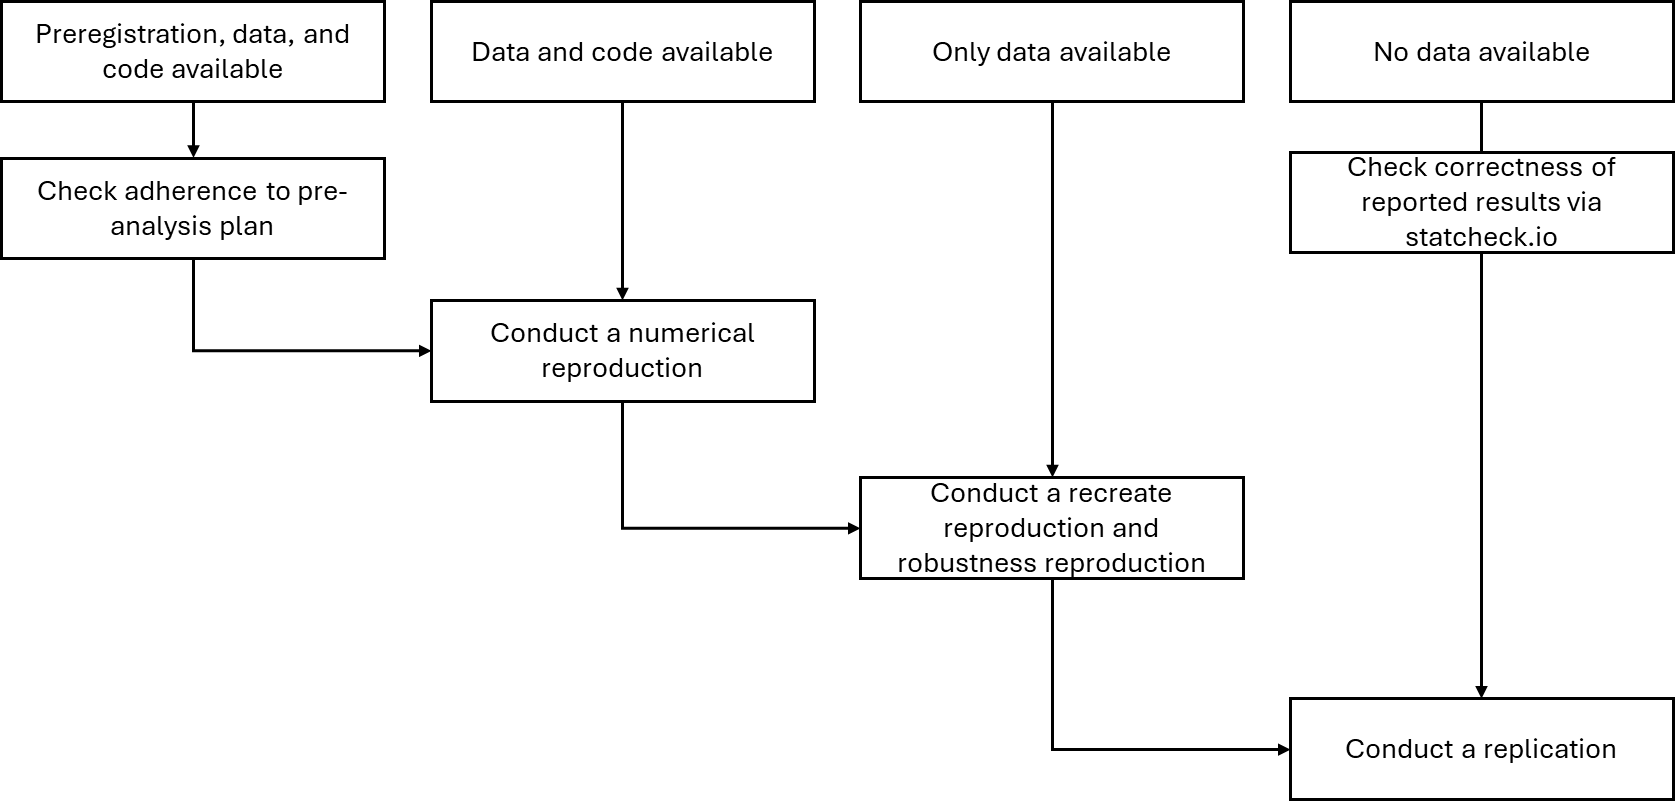
\includegraphics[keepaspectratio]{images/WBn_Image_3.png}}

}

\end{figure}%

\section{Close replication before conceptual
replication}\label{close-replication-before-conceptual-replication}

If the goal is to increase the generalizability of a specific finding,
we also suggest starting with replications that adhere as close as
possible to the original study (e.g., close replications) and only later
conduct conceptual replications. Based on Hüffmeier, Mazei, and Schultze
(\citeproc{ref-HueffmeierEtAl2016}{2016}), we propose the typology and
order of replication attempts in Figure~\ref{fig-replication-sequence}.
Importantly, replications at any stage should not compromise any aspects
of an original study, but rather---at the latest from the third study
stage (constructive replications) onwards---try to improve one or more
aspects of the original study, such as ``{[}\ldots{]} more valid
measures, more critical control variables, a more realistic task, a more
representative sample, or a design that allows for stronger conclusions
regarding causality'' (\citeproc{ref-KohlerCortina2021}{Köhler and
Cortina 2021, 494}). Köhler and Cortina term such replications
``constructive replications'' and caution against the conduct of
``quasi-random'' replications that vary features without clear
rationale.

Finally, there may be cases where the sequence of replications is not
necessary, or where the context of the replication team requires a focus
on generalisability to a specific context (see
Section~\ref{sec-differences-and-interpretation}).

\begin{figure}

\caption{\label{fig-replication-sequence}Sequence of replications from
exact replications to conceptual replications under field conditions}

\centering{

\pandocbounded{
\includegraphics[keepaspectratio]{images/6sH_Image_4.png}}

}

\end{figure}%

Note: This is an adaptation and update of the typology of replication
studies by Hüffmeier, Mazei, and Schultze (2016). The typology is
conceptualized as a hierarchy of studies that together help to (i)
establish the validity and replicability of new effects, (ii) exclude
alternative explanations, (iii) test relevant boundary conditions, and
(iv) test generalizability.

\chapter{Execution of Reproductions}\label{execution-of-reproductions}

\section{Gathering resources}\label{gathering-resources}

Prerequisites for reproduction studies are available data and ideally
also code. These are usually linked within the manuscript and shared via
repositories (e.g., Zenodo, OSF.io, github.com, gitlab.com) or they are
part of the supplemental materials that are listed on the article's
website. In special cases, an entire original manuscript may be
reproducible and written in Markdown language. Researchers searching for
target studies to reproduce can check topfactor.org and filter for Data
transparency level 3 (\citeproc{ref-topfactorDataSharing}{Leibniz
Institute for the Social Sciences 2023}, will no longer be updated).
They can also use the extensive database of economics studies with
available data compiled by Sebastian Kranz
(\citeproc{ref-KranzDataList}{Kranz 2025}).

If data are not publicly available, researchers can contact the authors
of the original study. In this case, we recommend them to adhere to
\emph{Guide for Accelerating Computational Reproducibility in the Social
Sciences} (ACRE) guidelines for constructive communication
(\citeproc{ref-BITSS2020}{Berkeley Initiative for Transparency in the
Social Sciences 2020}).

When re-using data, researchers need to respect licenses. Generally,
research data should be licensed openly, that is re-use and alteration
should be permitted, likely requiring citation of the original resource
(e.g., CC-BY 4.0 Attribution). Note, however, that non-derivative
licenses may prohibit reproductions; in that case separate approval
would be required from the copyright holder.

When it comes to reporting, Ankel-Peters et al.
(\citeproc{ref-AnkelPetersEtAl2025}{2025}) provide a table for reporting
results from the computational reproduction that includes resource
availability (e.g., raw data, cleaning code, analysis code).

\section{Contacting Authors}\label{contacting-authors}

Reproduction authors may have to contact the original authors if there
is something missing. It will often be necessary to contact the authors
more than once because missing descriptions of details of the original
study only become apparent once the replication study is planned. In
most cases, the original paper identifies one of the authors as
``corresponding author'' with an e-mail address. We recommend a quick
web search to check if this is the current email address, as researchers
frequently change institutions and thus e-mail addresses. Sometimes, it
may be most helpful to write to the last authors instead, who tend to
have more stable e-mail addresses, or to copy all authors into the
email. Templates for asking for materials and sharing replication
results can be found in Section \textbf{?@sec-appendix\_templates}. Note
that original authors may not respond due to institutional changes or
not being active in academia anymore.

\section{Identification of Claims}\label{identification-of-claims}

Statistical analyses and their results are always used as a way to
evaluate a certain claim. While Ankel-Peters et al.
(\citeproc{ref-AnkelPetersEtAl2025}{2025}) recommend reproductions to
identify ``results {[}that{]} are essential for the paper's main
argument to hold``, we acknowledge that a reproduction can also focus on
secondary results if they are relevant in some other context. In either
case, reproduction researchers need to justify the choice of the claim
in their report

\section{Preregistration}\label{preregistration}

Preregistrations contain a description of the planned study or analysis
prior to their execution. This way, they can reduce researchers'
`degrees of freedom'. In the case of reproductions, they can prevent
QRPs (e.g., ``null hacking,'' \citeproc{ref-BryanEtAl2019}{Bryan,
Yeager, and O'Brien 2019}; ``gotcha bias,''
\citeproc{ref-BerinskyEtAl2021}{Berinsky, Druckman, and Yamamoto 2021})
as long as the entire analysis plan is preregistered
(\citeproc{ref-BrodeurEtAl2024a}{Brodeur, Cook, et al. 2024}) and the
data have not yet been accessed. While a numerical reproduction with
available code does not require preregistration, we recommend a priori
specification of all further planned analyses.

It should be noted that a preregistered analysis plan or analysis script
is much easier to create with access to data and reproductions are
impossible with unavailable data, preregistration cannot exclude the
risk of authors having already looked at the data, yet making fraudulent
claims regarding data access in a preregistration is evidently academic
misconduct. How much weight readers and reviewers will give to a
preregistration based on data that could have been accessed already will
differ, but generating it is a way to keep ourselves accountable and
produce robust reproductions.

\section{Deviations}\label{deviations}

To increase trust in the reported results, reproduction researchers need
to report them in a transparent way, in a possible preregistration and
the final report. Ideally, all changes to the original procedure are
explained, justified, and hypotheses about their expected effect on the
outcomes are reported. Note that some journals' publishing reproductions
require adherence to special requirements such a Registered Report
format (e.g., \emph{Journal of Open Psychology Data}) or including a
minimum of two independent reproductions (e.g., \emph{Journal of
Robustness Reports}).

\section{Analysis}\label{analysis}

The main part of the reproduction is the analysis. Factors that are
potentially relevant for reproduction success include the software of
the machine that is running the code as well as versions of the software
and additional packages or plug-ins. For example, users of the open
source software R can get a comprehensive overview of the program
version and their machine using the function sessionInfo(), which should
be included in supplementary materials. For python users, a package has
been developed to run a similar function session\_info.show()
(\url{https://gitlab.com/joelostblom/session_info}).

Apart from a numerical reproduction where the same code is used,
reproduction researchers can explore alternative ways that should and
should not affect the results, test new hypotheses or theories, and run
exploratory analyses. Their report should be clearly structured to
discern these methods. Finally, for statistical analyses, the
reproduction report should include reproducibility indicators
(\citeproc{ref-DreberJohannesson2024}{Dreber and Johannesson 2024}) that
summarize statistical significance and relative effect sizes across the
original and reproduction results. Ankel-Peters et al.
(\citeproc{ref-AnkelPetersEtAl2025}{2025}) recommend a visual summary of
these indicators in the form of a reproducibility dashboard and
specification curves Mazei, Hüffmeier, and Schultze
(\citeproc{ref-MazeiEtAl2025}{2025}). We strongly recommend reproduction
researchers to consult the respective resources for further details.

\section{Discussion}\label{discussion}

The discussion section should include a clear evaluation of the
reproduction success on different levels
(\citeproc{ref-AnkelPetersEtAl2025}{Ankel-Peters et al. 2025}).
Researchers should report possible reasons for failure (e.g., objective
coding errors, changes in software packages) and the role of differences
between the original and the reproduction studies' results with respect
to their conclusions. Finally, if the original authors provided
comments, the reproduction report should include a discussion of them.

\chapter{Execution of Replications}\label{execution-of-replications}

\section{Preregistration and Registered (Replication)
Reports}\label{preregistration-and-registered-replication-reports}

Due to the replications being met with skepticism, we encourage
researchers to adhere to the highest standards of openness and
transparency. This includes preregistering the replication including the
analysis plan (ideally with an analysis code that was tested beforehand
using data from test runs or simulations), and criteria for the results
to distinguish between a replication success and failure. A
preregistration without an analysis plan provides no safeguard against
\emph{p}-hacking (\citeproc{ref-BrodeurEtAl2024a}{Brodeur, Cook, et al.
2024}). Beware that these criteria can be structured sequentially. For
example, if there is a manipulation check, it can be defined that it has
to work for the replicability to actually be evaluated. Boyce et al.
(\citeproc{ref-BoyceEtAl2024}{2024}) also found that repeating
unsuccessful replications did not change the outcomes unless obvious
weaknesses were fixed.

There is a specific preregistration template by Brandt et al.
(\citeproc{ref-BrandtEtAl2014}{2014}) but it may not fit the structure
of some studies beyond social psychology (e.g., personality science or
cognitive psychology; for a list of preregistration templates see
\url{https://osf.io/7xrn9} and \url{https://osf.io/zab38/wiki/home}). To
facilitate publication of the replication, we furthermore encourage
submitting it as a Registered Report. A rejection due to the results is
not possible at this point. A list of journals offering Registered
Reports (irrespective of replications) is
\href{https://docs.google.com/spreadsheets/d/1D4_k-8C_UENTRtbPzXfhjEyu3BfLxdOsn9j-otrO870/edit\#gid=0}{available
online}.

A special review platform for Registered Reports is \emph{Peer Community
in Registered Reports} (PCI-RR; \url{https://rr.peercommunityin.org})
where a community reviews pre-prints. Once accepted by PCI-RR, authors
can decide to publish their paper in participating journals (PCI
friendly journals) without another editorial round.

Finally, replication researchers need to deal with deviations from their
preregistration in a transparent way. In principle, there is nothing
wrong with deviating from what one had planned but most importantly, all
changes should be listed, discussed, and it should be made transparent
how the changes affected the results (for recommendations on changes and
documentation, see Lakens (\citeproc{ref-Lakens2024}{2024}), and
Willroth and Atherton (\citeproc{ref-WillrothAtherton2024}{2024}). If
changes are noticed during the data collection, many platforms also
allow the upload of amendments with preserved version history.

\section{Sample Size Determination}\label{sample-size-determination}

For replication studies, power analyses or other types of sample size
justification can be simpler than for studies testing entirely new
hypotheses because there already is a study that did what one is
planning, with a result that one can refer to. However, we advise
against simply using the original study's sample size. While the maxim
for most decisions is ``stay as close as possible to the original
study'', sample sizes of replication studies usually need to be larger.
To be informative, replication failure should provide evidence \emph{for
}a null hypothesis or a substantially smaller effect size, which
requires a larger sample. While a general tutorial for sample size
justification is provided by Lakens (\citeproc{ref-Lakens2022b}{2022}),
we briefly present approaches that are fit for replication studies.

As a pair of original and replication studies is usually concerned with
multiple effect sizes (e.g., for different
scales/items/groups/hypotheses), their number and individual power need
to be considered carefully. If the interpretation will rely on the
significance of \emph{all }effect sizes, the total power will be smaller
than the power for each individual test. To get along with limited
resources, researchers may choose one single effect size and argue that
it is central, or clearly specify other methods for aggregation across
results (e.g., testing multivariate models).

\subsection{Small Telescopes Approach}\label{small-telescopes-approach}

The idea behind the small telescopes approach
(\citeproc{ref-Simonsohn2015}{Simonsohn 2015}) is that a replication
study should be precise but how far this precision exceeds the original
study should be limited. Specifically, the replication study should be
able to detect an effect size for which the original study had
insufficient power (usually 33\%). If that effect size can be ruled out,
the original study can be treated as uninformative, as with such low
power, the result becomes more likely to have been a false positive.

This approach is based on the notion that replications should assess the
evidentiary value of the original study, and that the `burden of proof'
shifts back to proponents of a hypothesis if their evidence is shown to
be very weak. It is particularly appropriate when original studies are
very imprecise. In that case, a replication that finds a much smaller
effect may well still be compatible with the (wide) confidence interval
of the original study, and it might be impossible to reject the original
claim on that basis.

As an example, Schultze, Gerlach, and Rittich
(\citeproc{ref-SchultzeEtAl2018}{2018, fig. 4}) found an effect in three
studies with an average effect size of \emph{r} = -.11, 95\% CI {[}-.22,
-.01{]}.

If we wanted to achieve high power to rule out an effect of -.01, and
thus show that the true effect does not fall into their confidence
interval, we would need a sample size of 108,218 participants (alpha =
5\%, one-tailed test\footnote{Note that a two-tailed test could be
  applied as well. Given that the original study has a clear effect and
  direction, one-tailed gives the original authors the benefit of the
  doubt.} ). Conversely, with the small telescopes approach, we would
aim to test whether the replication effect is \emph{smaller} than the
effect which the original study had 33\% power to detect, \emph{r }=
-.043 (alpha = 5\%, one-tailed test). Simonsohn
(\citeproc{ref-Simonsohn2015}{2015}) showed that this requires a sample
2.5 times as large as the original for 80\% power. However, we deem that
level of power insufficient for replications, and instead suggest aiming
for 95\% power (given that a false negative in a replication leads to a
wrong claim regarding the absence \emph{of an effect}). This requires a
multiple of 4.5 (rather than 2.5, see
\citeproc{ref-Wallrich2025}{Wallrich 2025}), so a sample is in this case
of 4.5 * 793 = 3,569 participants. If this replication then results in
an estimate that is \emph{significantly smaller }than the effect the
original study had 33\% power to detect, the small telescopes approach
would suggest treating the original study as unable to provide reliable
evidence for its claim.

\subsection{Equivalence Testing}\label{equivalence-testing}

If statements can be made about the smallest effect size of interest
(SESOI), researchers can aim to test whether the replication effect is
smaller than that. Given that the direction is fixed by the original,
this simply requires running a one-sided test, e.g., a \emph{t}-test in
the case of a two group design, in the ``lesser'' direction. If the
replication effect size is significantly smaller than the SESOI, the
original claim is taken to be refuted in this instance by those who
accept that this is really the smallest effect of interest. Lakens et
al. (\citeproc{ref-LakensEtAl2018}{2018}) provide a practical tutorial
on equivalence testing, though they focus on cases where observations in
either direction would falsify the null hypothesis.

\subsection{Bayesian Approach}\label{bayesian-approach}

External knowledge can be incorporated into sample size planning
(uninformative / flat priors; heterogeneity; shrinkage) using the R
package BayesRepDesign (\citeproc{ref-PawelEtAl2023}{Pawel, Consonni,
and Held 2023}). Moreover, Micheloud and Held
(\citeproc{ref-MicheloudHeld2022}{2022}) provide a method for
incorporating an original study's uncertainty into power calculations.
With interim analyses (e.g., sequential testing) , a replication study
can also be stopped early and prevent wasting resources
(\citeproc{ref-WagenmakersEtAl2019}{E. J. Wagenmakers, Gronau, and
Vandekerckhove 2019}). However, when planning to use Bayes Factors to
make inferences about replication success, it is important to plan to
use plausibly narrow priors. Priors that assign substantial likelihood
to effects rarely observed (e.g., N(0,1) priors for standardized mean
differences in the social sciences) may be taken to unfairly privilege
the null hypothesis, which is inappropriate for a study setting out to
find support for it.

\subsection{Meta-Analytical Estimates}\label{meta-analytical-estimates}

If the replication study is part of a larger research programme, it is
possible to include other studies in the estimate of the (minimum)
effect size one wishes to detect/rule out. The target study may be part
of a multistudy paper with at least one other study that includes an
effect size for the hypothesis of interest. Researchers can compare the
effect sizes and possibly pool them to get a more precise estimate (for
a related Shiny App, see \citeproc{ref-McShaneBockenholt2017}{McShane
and Böckenholt 2017}).

Metrics such as average effect sizes, heterogeneity, or the confidence
interval width are valuable estimates needed for the replication's
sample size justification. If there is a meta-analysis on the general
topic, researchers can also use that to inform sample size planning, but
should prioritise estimates that aim to correct for publication bias and
other QRPs (for an overview see \citeproc{ref-Nagy_2025}{Nagy et al.
2025}). They should also choose effect sizes from a set of studies that
resembles the planned replication study as closely as possible. For
correlational effects, researchers can check \url{metabus.org}
(\citeproc{ref-BoscoEtAl2017}{Bosco, Uggerslev, and Steel 2017}) to
identify similar studies.

\subsection{Multilab Replications}\label{multilab-replications}

Multilab replications, that is replications that are conducted by
different groups of researchers in different locations adhering to the
same protocol, allow researchers to investigate heterogeneity of effects
and estimate effect sizes with high precision. There are currently no
standards for planning sample sizes for multilab replications. Depending
on the specific goals, a power analysis needs to account for possible
moderator hypotheses and the desired precision of effect size,
heterogeneity estimates, or cultural variables. Note that this often
requires large sample sizes for any level of the moderator (e.g.,
culture, profession). Usually, the different labs are required to
collect data from a minimum number of participants. Each lab's study and
all analysis scripts should be preregistered to prevent local and global
QRPs such as optional stopping or ad hoc exclusions of single labs.

\section{Changes in the Methods}\label{changes-in-the-methods}

A replication study should closely resemble the original study, in the
case of conducting a direct/close replication. However, this is
difficult for multiple reasons: First, original studies may not include
sufficient detail to allow for a replication
(\citeproc{ref-AguinisSolarino2019}{Aguinis and Solarino 2019};
\citeproc{ref-ErringtonEtAl2021a}{Errington, Denis, et al. 2021}).
Second, scientific progress in the form of new methods and insights and
cultural changes might require replication researchers to make changes
or additions to their study. Third, obvious errors must be corrected. We
elaborate on a number of reasons to deviate from an original study. In
the replication report, all deviations should be reported and justified
exhaustively.

\begin{itemize}
\item
  {Unspecific original materials:} If the original study does not
  specify a key element that is needed for the replication, replication
  researchers can reach out to the original study's authors and ask for
  the details. If this is not possible because authors cannot be reached
  or they are unwilling/unable to share the materials, new materials
  must be created. In this case, special attention should be paid to the
  theory, so that the new materials exhibit both face and construct
  validity.
\item
  {Deprecated materials:} If a psychological study about person
  perception published in the 1980s used celebrities, the examples used
  may no longer have the same status. For example, Mussweiler et al.
  (\citeproc{ref-MussweilerEtAl2000}{2000}) used ``a 10-year old car
  (1987 Opel Kadett E)'' to be evaluated in German Marks. For a new
  study, car and currency would have to be replaced as a car's age is
  strongly associated with price. Like most studies, the original
  provides no details about the conditions that a new stimulus would
  have to meet. Ideally, the theoretical requirements for stimuli should
  be specified in primary research, where they are not, replication
  authors need to make their own assumptions and report them explicitly
  (see \citeproc{ref-SimonsEtAl2017}{Simons, Shoda, and Lindsay 2017}).
\item
  {Translation:} Most published original studies are in English. If the
  replication sample's mother tongue is not English, translation may be
  necessary. Standards for translation differ strongly even between
  subfields. For example, when a personality scale is translated, the
  translated version will usually be validated and tests of invariance
  will be required. In social psychology, such procedures are less
  common, and often merely a back-translation is conducted. However, in
  any field, measurement invariance is required if one wants to compare
  effect sizes across samples, so that this should be tested rather than
  assumed where possible.
\item
  {Necessity of a special sample:} Many large-scale replication projects
  made use of click workers (e.g., via MTurk) or use student samples.
  Replicators should consider if using such samples satisfy their needs
  and evaluate which platform to use (for best practices and ethical
  considerations, see Kapitány and Kavanagh
  (\citeproc{ref-KapitanyKavanagh2023}{2023}). Even if the original
  study used such a convenience population, changing to a different
  convenience population may require tweaks to maintain comparability,
  e.g.~with regard to participant attentiveness and engagement with the
  paradigm.
\item
  {Quality of methods and apparatus:} Replicating old studies often
  faces the problem that something new has been discovered that should
  be taken into account. If a specific tool or method is used, there may
  be another recent method that is more reliable. For example, software
  for eye tracking studies from the early 2000s is now deprecated; there
  is new hardware and software that researchers will use. This might
  also apply to analysis methods, yet where possible, both the results
  from the original methods as well as state-of-the-art methods should
  be reported; where a choice has to be made, it is essential that
  invalid methods are avoided while comparability is maintained as far
  as possible. Finally, if the original finding's generalizability is
  tested, new items or tasks that vary more or less systematically can
  be added to compare results for the original parts versus these
  extensions (though order effects have to be carefully considered, as a
  second manipulation might affect participants differently from a first
  manipulation)
\item
  {Adding checks:} Doing a replication often implies some uncertainty in
  the results, so it is wise to include checks that will be helpful to
  interpret the results, especially if they are negative. For example,
  if there are occurrences that would make the results meaningless, it
  is good to have a way to measure them and incorporate that into the
  study. This could include positive or negative controls (items that
  are diagnostic of the method rather than the question of interest),
  manipulation checks (generally placed \emph{after }the critical parts
  of the experiment), or attention checks. See Frank et al.~(2025,
  \href{https://experimentology.io/012-collection.html\#ensuring-high-quality-data}{chapter
  12.3}) for further discussion.
\end{itemize}

\section{Piloting}\label{piloting}

If considerable resources are linked to the full execution of a
replication (e.g., in a Registered Replication Report), or when new
materials are used, researchers may want to consider piloting it (or
parts of it) first. For multi-lab replications, researchers may want to
consider a sequential study order in contrast to a simultaneous design:
As Buttliere (\citeproc{ref-Buttliere2024}{2024}) put it: ``Who gets
better results, 39 people doing it the first time or one person doing it
39 times?'' (p.4) Beware that piloting may not be of value if it is
simply an under-powered version of the study; instead it may be used to
identify flaws in the methodology or test assumptions about the
distribution of values or participants' qualitative responses.
Importantly, small pilot studies should never be used to derive effect
sizes for power analyses as their results are too imprecise.

For instance, researchers should follow general best practices for their
replications including piloting their study on a few participants to
ensure that the instructions are clear, that the procedure works
smoothly (e.g., website loads appropriately), and that all necessary
data are recorded. A debriefing survey where pilot participants are
asked about their experience, the clarity of instructions, and the
clarity of any user interface, can help to identify some issues that
could undermine the replication. See Frank et al.~(2025, chapter 12.3.1)
for further discussion on piloting studies.

\subsection{Collaborating and Consulting with the Original
Authors}\label{collaborating-and-consulting-with-the-original-authors}

To reduce the chance that a failure to replicate is dismissed by the
original study's authors afterwards by pointing out a flaw in the
method, researchers can consult with the original authors before running
the study. However, in the past, this still has not kept the original
authors from dismissing a replication as an inadequate test of a
hypothesis (\citeproc{ref-BaumeisterVohs2016}{Baumeister and Vohs
2016}). Note that replication researchers have even been accused of
``null hacking'' (\citeproc{ref-Protzko2018}{Protzko 2018}) although
little evidence exists for this claim
(\citeproc{ref-BerinskyEtAl2021}{Berinsky, Druckman, and Yamamoto
2021}). While involving original authors can help in creating a good
study when reporting is poor, ideally original studies should be
reported in sufficient detail for others to replicate them without
further involving the original authors. Historically, the relationship
between involvement of original authors and the average replication
effect size is not clear (although there have been lab effects in some
cases (\citeproc{ref-PowersEtAl2013}{Powers et al. 2013}). This is
showcased here in a few examples:

\begin{itemize}
\item
  Powers et al. (\citeproc{ref-PowersEtAl2013}{2013}) investigated the
  effect of video games on information processing and found larger
  effect sizes for active research groups.
\item
  Ten effects from Open Science Collaboration
  (\citeproc{ref-OpenScienceCollab2015}{2015}) were replicated in Many
  Labs 5 (\citeproc{ref-EbersoleEtAl2020}{Ebersole et al. 2020}), where
  the original authors commented on the study protocols of the planned
  replication before these replications were conducted, and ``the
  revised protocols produced effect sizes similar to those of the RP:P
  protocols (Δr = .002 or .014, depending on analytic approach).''
\item
  McCarthy et al. (\citeproc{ref-McCarthyEtAl2021}{2021}) conducted a
  multisite replication of hostile priming where one of the original
  authors was involved. Each laboratory conducted a close and a
  conceptual replication and found no difference and recommended that
  ``researchers should not invest more resources into trying to detect a
  hostile priming effect using methods like those described in Srull and
  Wyer (1979)''.
\item
  After Baumeister and Vohs (\citeproc{ref-BaumeisterVohs2016}{2016})
  criticized the failed registered replication report by Hagger et al.
  (\citeproc{ref-HaggerEtAl2016}{2016}) for their methods, Vohs et al.
  (\citeproc{ref-VohsEtAl2021}{2021}) conducted another registered
  replication report and also found a null effect.
\item
  After no effect of the pen-in-mouth task was found in the facial
  feedback Registered Replication Report by Wagenmakers et al.
  (\citeproc{ref-WagenmakersEtAl2016}{2016}), another multilab test,
  which included one of the original authors, arrived at the same
  results (\citeproc{ref-ColesEtAl2022}{2022}).
\item
  The Many Labs 4 project set out to test the effect of author
  involvement on replication success but found an overall null effect
  for the group of studies that did and that did not include original
  findings' authors (\citeproc{ref-KleinEtAl2014}{Klein et al. 2014}).
\item
  For social priming studies' replication success, ``the strongest
  predictor of replication success was whether or not the replication
  team included at least one of the authors of the original paper''
  (\citeproc{ref-MacGiollaEtAl2024}{Mac Giolla et al. 2024}).
\end{itemize}

\section{Adversarial Collaborations}\label{adversarial-collaborations}

Although they are not specific to replication projects, researchers have
often issued calls for adversarial collaborations
(\citeproc{ref-ClarkEtAl2022}{Clark et al. 2022};
\citeproc{ref-CowanEtAl2020}{Cowan et al. 2020};
\citeproc{ref-CorcoranEtAl2023}{Corcoran, Hohwy, and Friston 2023}).
Thereby, groups of researchers can collaborate and try to settle
conflicting views by designing and conducting a study designed to settle
a debate. A related idea are ``red teams'' where experts are invited to
critique the analysis plan, without becoming authors and thus without a
conflict of interest in terms of desired results
(\citeproc{ref-LakensEtAl2018}{2018}).

\section{Analysis}\label{analysis-1}

Analyses of replication results are often a compromise or a combination
of the original analysis and the current state-of-the-art. Generally,
replication studies should follow the original analysis plan as closely
as possible. That does not only concern statistical procedures but also
data processing (e.g., exclusion of outliers, transformation and
computation of variables). Even when following the original analysis
plan for their confirmatory analysis, researchers should still follow
best practices and examine their raw data to check for distributional
anomalies to detect whether participants might be inattentive, guessing
or speeding, and report relevant sensitivity checks where helpful. Some
things to check for include theory-agnostic condition/manipulation
checks (e.g., were participants faster in the condition focused on
speed?) and the results of attention checks or control trials.
Generally, it is advisable not to remove participants from the main
analysis on that basis, but instead to confirm that the rates of
non-compliance are acceptably low and to report robustness to the
exclusion of these participants. See Ward and Meade
(\citeproc{ref-WardEtAl2023}{2023}) for a comprehensive review of
strategies for assessing and responding to careless responding.

At times, methodological advances may suggest that the original
statistical tests are not robust. In such cases, researchers may want to
run both the test that the original study used, as well as the
statistical approach that is most appropriate by today's standards (for
instance, both the \emph{t}-test that can be compared with the original,
and the mixed-effect model that is justified by the study design). Where
original data is available, or can be obtained from the original
authors, researchers might be able to also update the analyses in the
original study, which facilitates interpretation.

Where original statistical analyses are fundamentally flawed,
replication researchers are faced with a difficult choice. For instance,
it has been convincingly demonstrated that the famous Dunning-Kruger
effect (\citeproc{ref-KrugerEtAl1999}{Kruger and Dunning 1999}) is based
on analyses strongly influenced by a statistical artifact, namely
regression to the mean (\citeproc{ref-GignacEtAl2020}{Gignac and
Zajenkowski 2020}). In such a context, one may want to report results
based on the original methods alongside more robust tests, yet needs to
be very careful to frame them in a way that ``replication success''
cannot be claimed in the absence of evidence for the original claim.

Exclusion criteria are another area where there may be tension between
the original study and current best practices. Typically, it makes sense
to run the analysis both ways to check for robustness, yet one analysis
choice should be preregistered as the central analysis.

Naturally, original and replication results should be compared.
Unstandardized values can be informative with respect to sample
characteristics (e.g., overall reaction times). How to do this
analytically depends on the choice of success criteria discussed in the
next section.

\chapter{Discussion}\label{discussion-1}

\section{Defining and Determining Replication
Success}\label{sec-success-criteria}

There is no strong consensus yet on what constitutes a replication
success and some approaches can be biased
(\citeproc{ref-SchauerHedges2021}{Schauer and Hedges 2021}) or imprecise
(\citeproc{ref-PatilEtAl2016b}{Patil, Peng, and Leek 2016b}). Like in
classical null hypothesis significance testing (NHST), replication
researchers face the trade-off between dichotomizing something that is
not dichotomous (success vs.~failure) and making a clear decision about
the outcome. On the one hand this is a question about statistical
choices and their interpretation, namely how to compare original and
replication effect sizes (or \emph{p}-values) and how to interpret
differences. On the other hand, it is a more complex question about how
to interpret a mixed pattern of results, where some results are
consistent across original and replication, while others are not. Here,
it is important for replication researchers to specify which effects are
of primary interest in their preregistration, and how they will
aggregate results, noting that requiring multiple effects to yield the
same result will reduce statistical power.

Below, we present different approaches to assessing replication success
as summarized by Heyard et al. (\citeproc{ref-HeyardEtAl2025}{2025}; see
also \citeproc{ref-MuradchanianEtAl2021}{Muradchanian et al. 2021};
\citeproc{ref-RoselerWallrich2024}{Röseler and Wallrich 2024};
\citeproc{ref-ErringtonEtAl2021a}{Errington, Denis, et al. 2021}, Table
1)

\begin{longtable}[]{@{}
  >{\raggedright\arraybackslash}p{(\linewidth - 4\tabcolsep) * \real{0.1784}}
  >{\raggedright\arraybackslash}p{(\linewidth - 4\tabcolsep) * \real{0.5671}}
  >{\raggedright\arraybackslash}p{(\linewidth - 4\tabcolsep) * \real{0.2545}}@{}}

\caption{\label{tbl-rep-success-criteria}Criteria to operationalize
replication success (excerpt from Heyard et al.
(\citeproc{ref-HeyardEtAl2025}{2025}, Table 4)) For full references and
descriptions, see the
\href{http://rachelheyard.com/reproducibility_metrics/\#table}{original
table}. Reused in accordance with the CC-BY license of the article.}

\tabularnewline

\toprule\noalign{}
\begin{minipage}[b]{\linewidth}\raggedright
Name
\end{minipage} & \begin{minipage}[b]{\linewidth}\raggedright
Question answered
\end{minipage} & \begin{minipage}[b]{\linewidth}\raggedright
Type of Reproducibility investigated
\end{minipage} \\
\midrule\noalign{}
\endhead
\bottomrule\noalign{}
\endlastfoot
Bayes Factor: Independent Jeffreys-Zellner-Siow BF test & ``What is the
evidence for the effect being present or absent in light of a
replication attempt, given that we know relatively little about the
expected effect size beforehand?'' & Different data - same analysis \\
Bayes Factor: Equality-of-effect-size BF test & ``What is the evidence
for the effect size in the replication attempt being equal vs.~unequal
to the effect size in the original study?'' & Different data - same
analysis \\
Bayes Factor: Fixed-effect meta-analysis BF Test & ``When pooling all
data, what is the evidence for the effect being present vs.~absent?'' &
Different data - same analysis \\
Replication Bayes factor & ``What is the evidence for the effect from
the replication attempt being comparable to what was found in the
original study, or absent?'' - ``Are the replication results more
consistent with the original study or with a null effect?'' & Different
data - same analysis \\
Significance criterion & ``Do the original and replication study both
find a statistical significant effect in the same direction?'' &
Different data - same analysis; Same data - different analysis;
Different data - different analysis \\
Difference in effect size & ``To which degree do the effects from a
replication study mirror the original'' & Different data - same
analysis; Same data - different analysis; Different data - different
analysis \\
Confidence interval: original effect in replication 95\% CI & ``Given an
original effect size, (what is the probability that) does a repetition
of the experiment, with an independent sample of participants,
produce(s) a CI that overlaps with the original effect?'' & Different
data - same analysis \\
Confidence interval: replication effect in original 95\%CI & ``Given an
effect size and 95\% CI, (what is the probability that) does a
repetition of the experiment, with an independent sample of
participants, give(s) an effect that falls within the original CI?'' &
Different data - same analysis \\
Prediction interval: replication effect in original 95\% prediction
interval & ``Do the findings from the replication study align with a
reasonable expectation, given the observed variation in the original
study and replication study?'' - ``Are the replication estimates
statistically consistent with the original estimates?'' & Different data
- same analysis \\
Small Telescopes & ``Are the replication results consistent with an
effect size big enough to have been detectable in the original?'' &
Different data - same analysis \\
Meta-analysis & ``Given an original-replication study pair, does the
pooled effect align with that of the original study?'' - ``Given a set
of replications, is the effect size reproducible across studies?'' &
Different data - same analysis; Same data - different analysis;
Different data - different analysis \\
Equivalence testing & ``For the replication of an original null finding,
does the replication study find an effect that is equally negligible?''
- ``Are the results from the replication statistically equivalent to the
results of the original study?'' & Different data - same analysis \\
Minimum effect testing & ``Is the replication effect size significantly
different from a minimal effect size of interest, required to support
the original study?'' & Different data - same analysis \\
Causal replication framework & ``How can a replication failure be
interpreted, from a causal perspective'' & Different data - same
analysis; Different data - different analysis \\
Text-based machine learning model to estimate reproducibility & ``Given
the text of an original paper, what is the probability of replication
success?'' & Different data - same analysis \\
Prediction market & ``What do the participants in a prediction market
predict as the probability that the original findings will replicate?''
& Different data - same analysis \\
Presence/Absence of elements ensuring reproducibility,via proxies & ``Do
the design, methods and reporting of the original paper align with
community standards of reproducible and transparent research?'' & Same
data - same analysis; Same data - different analysis; Different data -
same analysis; Different data - different analysis \\
Quantified reproducibility assessment, QRA & ``After performing multiple
measurements of an object, what is the precision of the measured
quantity obtained?'' & Same data - same analysis; Different data - same
analysis; Same data - different analysis; Different data - different
analysis \\
Jaccard similarity coefficient & ``By what extent do the results of two
(or more) fMRI experiments overlap?'' & Same data - same analysis \\
Sceptical \(p\)-value & ``To what extent are the results of a
replication study in conflict with the beliefs of a sceptic of the
original study?'' & Different data - same analysis \\
Modified Brinley plot & ``Given a pre-specified desired effect and
multiple replications, what is the share of replications that,
represented graphically, achieve the desired effect?'' & Same data -
same analysis; Same data - different analysis; Different data - same
analysis; Different data - different analysis \\
Likelihood-based approach for reproducibility & ``Given a theoretically
interesting effect size derived from the original study, what is the
evidence for or against replicating this effect?'' & Different data -
same analysis \\
Bayesian mixture model for reproducibility rate & ``Given the results
(\(p\)-values) from a set of original and replication studies, what is
the rate of reproducibility, and how is it related to certain aspects of
the experiments?'' & Different data - same analysis \\
Unified framework for estimating the credibility of published research &
``For a specific published research work, what is the evidence for its
credibility measured on four different dimensions: method and data
transparency, analytic reproducibility, analytic robustness and effect
reproducibility?'' & Same data - same analysis; Same data - different
analysis; Different data - same analysis; Different data - different
analysis \\
Reproducibility scale of workflow execution - Tonkaz & ``Given a certain
original research paper with results based on computation, can the
workflow to generate the results be executed and verified?'' & Same data
- same analysis; Same data - different analysis; Different data - same
analysis; Different data - different analysis \\
Mean relative effect size & ``What is the average ratio of replication
study effects to original study effects?'' & Different data - same
analysis; Same data - same analysis \\
Correlation between effects & ``Do the replication studies and the
original studies produce effects that are correlated?'' & Different data
- same analysis; Same data - same analysis \\
Fragility Index & ``Given the results of an original study were
significant, what is the smallest change in the original data that is
needed to deem the results non-significant? and vice-versa for original
null results'' - ``How fragile are the original results to small changes
in the underlying data?'' & Same data - different analysis \\
Externally standardized residuals & ``Is the original study consistent
with the replication(s)?'' - ``Are all studies included in a
meta-analysis replicable?'' & Different data - same analysis; Same data
- different analysis \\
Snapshot hybrid & ``After replicating an original study, what is the
evidence for a null, small, medium or large effect?'' & Different data -
same analysis \\
Bayesian Evidence Synthesis & ``Given several conceptual replications
with substantial diversity in data, design and methods but investigating
the same theory, what is the evidence underlying a certain theory of
interest?'' & Different data - different analysis \\
Design analysis & ``Given the results of an original study and an effect
of a hypothetical replication study, what is the probability of the
estimate being in the wrong direction, and what is the factor by which
the magnitude of the effect is overestimated?'' & Different data - same
analysis \\
Reproducibility Maps & ``For fMRI research, how many and which of the
truly active voxels were strongly reproduced?'' & Same data - same
analysis; Same data - different analysis \\
Continuously cumulating meta-analytic approach & ``Given subsequent
replications that were performed to date, what is the current evidence
for an effect?'' & Different data - same analysis \\
Correspondence test & ``To what extent does the effect size from the
replication study differ or is equivalent to that of the original
study?'' & Different data - same analysis \\
Z-curve & ``Do all studies combined provide credible evidence for a
phenomenon?'' & Different data - same analysis \\
Cross-validation methods & ``To what extent can the stability of a
result be trusted, and to what extent can the result be generalized?'' &
Different data - same analysis \\
Network Comparison Test, NCT & ``Given two network structures, how
similar are they to each other?'' & Same data - same analysis; Different
data - same analysis \\
Leave-one-out error & ``Given a deep learning model, how generalizable
are its results?'' & Different data - same analysis \\
Subjective reproducibility assessment & ``Does the replication team
consider the replication as successful?'' - ``To what extent does the
replication team trust in the reproducibility of a finding?'' &
Different data - same analysis \\
I squared - \(I^2\) & ``Given a set of replications, to what extent is
the total variation across study results due to heterogeneity?'' - ``How
consistent are the results across replications?'' & Different data -
same analysis; Different data - different analysis \\
Credibility analysis & ``How credible are the results of a study, in a
Bayesian framework?'' & Different data - same analysis \\
Consistency of original with replications, \(P_{\mbox{orig}}\) & ``To
what extent are the replication effect sizes consistent with the effect
size of an original study?'' & Different data - same analysis; Different
data - different analysis \\
Proportion of population effects agreeing in direction with the
original, \(\hat{P}_{>0}\) & ``To what extent do the replication effect
sizes agree with the sign found in the original study?'' & Different
data - same analysis; Different data - different analysis \\
RepliCATS & ``How reliable do experts believe the claims from an
original finding are?'' & Different data - same analysis \\
RepeAT - Repeatability Assessment Tool & ``Does the presented research
align with community standards of reproducible biomedical research,
using electronic health records?'' & Same data - same analysis;
Different data - same analysis \\
P interval & ``Given the results of an original study, what is the range
of \(p\)-values a replication (following the same design) would lie in
with 80\% probability?'' & Different data - same analysis \\
RipetaScore & ``Given certain trust in research, reproducibility and
professionalism quality indicators, how high does a paper score?'' &
Same data - same analysis; Different data - same analysis \\
Bland-Altman Plot & ``Do the effects estimated in several
original-replication study pairs agree with each other?'' - ``How good
is the agreement between repeated measures/studies?'' & Same data - same
analysis; Same data - different analysis; Different data - same
analysis; Different data - different analysis \\
Sceptical Bayes Factor & ``In light of the replication data, at which
level of evidence can an advocate of the original study convince a
sceptic?'' & Different data - same analysis \\

\end{longtable}

\section{Interpreting Divergent Results (Replication
Failures)}\label{interpreting-divergent-results-replication-failures}

When replications succeed, the original claim gains further credence (as
long as the methods are sound). However, when replications fail, many
explanations and interpretations can be advanced, which need to be
carefully considered and discussed in a report. While replication
failure can highlight issues with statistical conclusion validity in the
original studies (\citeproc{ref-JohnEtAl2012}{John, Loewenstein, and
Prelec 2012}; \citeproc{ref-NelsonEtAl2018}{Nelson, Simmons, and
Simonsohn 2018}; \citeproc{ref-SimmonsEtAl2011}{Simmons, Nelson, and
Simonsohn 2011}), other explanations need to be considered, including
issues with internal, external, and construct validity in both original
and replication studies (\citeproc{ref-FabrigarEtAl2020}{Fabrigar,
Wegener, and Petty 2020}; \citeproc{ref-VazireEtAl2022}{Vazire,
Schiavone, and Bottesini 2022}). For example, internal validity is
threatened when attrition rates differ between experimental conditions
in original or replication studies, creating potential confounds in the
interpretation of treatment effects (\citeproc{ref-ZhouFishbach2016}{H.
Zhou and Fishbach 2016}). Construct validity is threatened when original
or replication studies use unvalidated ad-hoc measures, fail to employ
validated manipulations of the target construct, or when differences in
sample characteristics between original and replication studies mean
that manipulations and measures do not work as intended
(\citeproc{ref-FabrigarEtAl2020}{Fabrigar, Wegener, and Petty 2020};
\citeproc{ref-FiedlerEtAl2021}{Fiedler, McCaughey, and Prager 2021};
\citeproc{ref-FlakeFried2020}{Flake and Fried 2020}). External validity
is threatened when original findings do not generalize to the specifics
of the replication study due to person and context differences between
studies that moderate the effect. Thus, before making statements about
the original finding's robustness and generalizability, replication
researchers need to critically discuss potential methodological
shortcomings in both original studies and replication attempts that
limit statistical conclusion, internal, external, and construct
validity.

\subsection{Hidden Moderator Account}\label{hidden-moderator-account}

One challenge for replication researchers is the identification of
hidden/unknown confounds that may influence or bias the phenomenon under
study. Each study has a set of potential extraneous or unknown moderator
variables that is unique to it. These may seem trivial, such as the
brightness of an experimental laboratory, or important, such as a
cultural difference between the replicating and original studies. Yet
even seemingly trivial differences \emph{could }potentially change
results. Often statistical and methodological choices are made to
circumvent or attenuate these issues. However, for some paradigms, these
variables could be unknown to the original researcher
(\citeproc{ref-Fiedler2011}{Fiedler 2011}). These are referred to in the
literature as unknown moderators, background variables, hidden
moderators or fringe variables. While they are always a way to reject
unpleasant replication results, they can potentially bias replications,
which highlights that a single replication is never entirely conclusive
(though it might raise enough doubts that researchers do not see the
value in addressing the remaining uncertainty). It should be noted that
the same argument \emph{could }be applied to raise doubts about any
original study, questioning whether the effect is really due to the
hypothesised cause or due to some hidden moderator or background
variable. Clearly a skeptic who stops at that level would not be taken
very seriously, so that it is important to move conversations about
replication failure beyond general suspicion of hidden moderators.

(\citeproc{ref-Bargh2006}{Bargh 2006}) suggested that the evidence
generated by empirical findings far outweighs the resources of (social)
psychology to conceptualize and understand the mechanisms underlying
their effects. Therefore, boundary conditions are not easily specified,
which can impact both direct and conceptual replication success.
Replication failure indicates that the original claim does not
generalise to the setting of the replication. Whether that generalises
to the setting of the original study needs to be considered in light of
theory, and might be a legitimate matter of contention.

\section{The Role of Differences for the Interpretation of
Findings}\label{sec-differences-and-interpretation}

Each replication outcome should be evaluated in the light of its
closeness, which is why all deviations with the respective reasons and,
if possible, their potential impact on the results should be discussed.
Existing theories may help assess whether a deviation should affect the
outcomes. For example, most psychological theories are agnostic towards
age so that a different distribution of participants' age will be
unproblematic in most cases. Researchers may choose to evaluate
replications from both phenomenon-focused / inductive and theory-focused
/ deductive views. Different types of interpretations are listed in
Figure~\ref{fig-success-interpretation} and integrated from previous
accounts by Borgstede and Scholz
(\citeproc{ref-BorgstedeScholz2021}{Borgstede and Scholz 2021}) and
Freese and Peterson (\citeproc{ref-FreesePeterson2017}{Freese and
Peterson 2017, fig. 3}).

\begin{figure}

\caption{\label{fig-success-interpretation}Interpretation of replication
outcomes depend on similarity of \textbf{closeness} and results as well
as the view (\textbf{inductive vs.~deductive}).}

\centering{

\pandocbounded{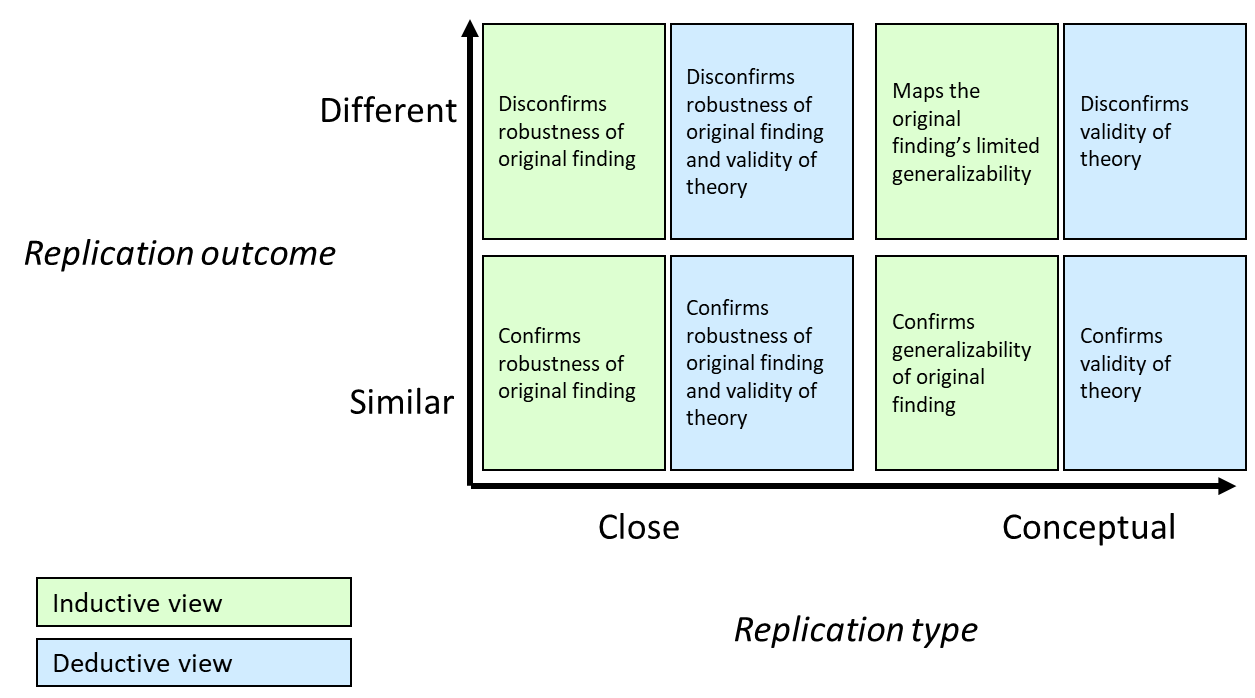
\includegraphics[keepaspectratio]{images/eH3_Image_5.png}}

}

\end{figure}%

\emph{Note.}

\begin{itemize}
\item
  Inductive or phenomenon-oriented views assume minimal generalizability
  of the original finding. For example, they cannot cast doubts on the
  original finding unless the replication is highly similar to the
  original study.
\item
  Deductive or theory-oriented views assume maximal generality of a
  theory. For example, different results (i.e., replication failures)
  cast doubts on the \emph{theory} regardless of the replication type.
\end{itemize}

\section{Comments from the Original Study's
Authors}\label{comments-from-the-original-studys-authors}

If the replication results do not converge with the original results,
replication researchers can reach out to the original study's authors
and ask for a comment that they can publish together with the
replication report. A template for asking for a comment is in the
appendix. Note that some journals (e.g., \emph{Journal of Replications
and Comments in Economics}) require such statements at the time of
submission.

\part{Advanced Topics and Applications}

\chapter{Communicating and
Publishing}\label{communicating-and-publishing}

The final step of replication research is publishing and communicating
the results. Researchers should adhere to best practices of transparency
and openness promotion guidelines (TOP,
\citeproc{ref-GrantEtAl2024}{Grant et al. 2024}) and to the reporting
standards of their respective field (e.g., JARS standards for reporting
psychology replications, \citeproc{ref-openpsychdataJARS}{Association,
n.d.}). For example, they should report a link to the preregistration,
analysis plan, and analysis script, share all materials and data (if
possible in light of ethical and legal limitations) under an open
license (see also \citeproc{ref-JanzFreese2021}{Janz and Freese 2021}),
and report methods and results comprehensively. Finally, in writing the
report, reproduction and replication authors should be mindful of their
language. Ideally, being replicated would be an honor for authors since
other researchers deem their findings important but a failed replication
could potentially harm the reputation of the original and increase
distrust towards them among their peers. We recommend a descriptive and
impersonal language. When criticizing bad documentation, no access to
data, or brevity in methods replication authors should keep in mind the
historical context of the original publication. For example, sharing
data was much more difficult in the 1990s and not required in many areas
until recently.

The journals that published the original studies are often also chosen
by authors for publication in accordance with the
\emph{pottery-barn-rule} (\citeproc{ref-Srivastava2012}{Srivastava
2012}). However, in our experience, many journals reject replications
due to their lack of novelty. We list several options for writing and
publishing the report in Table~\ref{tbl-reporting-options}. These are
non-exclusive, that is, researchers can choose multiple of them. An
overview of active journals that exclusively publish replications is in
Table~\ref{tbl-rep-journals}.

\begin{longtable}[]{@{}
  >{\raggedright\arraybackslash}p{(\linewidth - 2\tabcolsep) * \real{0.5000}}
  >{\raggedright\arraybackslash}p{(\linewidth - 2\tabcolsep) * \real{0.5000}}@{}}
\caption{Reporting and communicating reproductions and
replications.}\label{tbl-reporting-options}\tabularnewline
\toprule\noalign{}
\begin{minipage}[b]{\linewidth}\raggedright
Type
\end{minipage} & \begin{minipage}[b]{\linewidth}\raggedright
Description
\end{minipage} \\
\midrule\noalign{}
\endfirsthead
\toprule\noalign{}
\begin{minipage}[b]{\linewidth}\raggedright
Type
\end{minipage} & \begin{minipage}[b]{\linewidth}\raggedright
Description
\end{minipage} \\
\midrule\noalign{}
\endhead
\bottomrule\noalign{}
\endlastfoot
FORRT Replication Database & This open and collaborative database
contains thousands of replication findings and makes them visible.
Anyone can enter results using a guided survey
(https://t1p.de/fred\_submit). \\
PubPeer & Researchers can comment on the original study and say that
there is a replication attempt, describe the outcome, and provide
links/references/DOIs to the replication(s). Researchers checking
pubpeer.com or using the browser plug-in that automatically highlights
studies for which there are comments will see your comment. \\
Manuscript (required for Preprint and Journal Article) & Manuscripts are
mostly used as they are the traditional form of a research article. For
judgment and decision making, there are useful examples by Feldman
(\citeproc{ref-Feldman2024}{2024}). For reproducibility analyses the I4R
Replication Report Template (https://osf.io/j2qrx) can be used.
Moreover, Röseler et al. (\citeproc{ref-RoselerEtAl2025}{2025}) provide
general templates for reproductions and replications. \\
Preprint & We recommend publishing a report in the form of a traditional
or standardized manuscript as a preprint. This secures open access and
makes the report visible, citable, and commentable. There are many
preprint servers across the social sciences (e.g., PsyArxiv, SOCARXIV,
SportRxiv, MediArXiv, MindRxiv, EdArXiv, AfricArXiv, or MetaArXiv). In
some countries, researchers have a legal right for a secondary
publication of their research (green open access). Be aware that
preprints are faster in terms of publication than journal articles, but
are usually not peer-reviewed. \\
Journal article & Most researchers have to ``play by the rules'', that
is, publish or perish (\citeproc{ref-BakkerEtAl2012}{Bakker, Dijk, and
Wicherts 2012}; \citeproc{ref-KooleLakens2012}{Koole and Lakens 2012}).
While some have argued for a pottery barn rule where journals that
published the original finding have to publish respective replication
attempts (e.g., \citeproc{ref-Srivastava2012}{Srivastava 2012}), many
journals are not (yet) interested in replications. Notable exceptions
are listed in the appendix. This is why journals dedicated to
replications have emerged (see Table~\ref{tbl-rep-journals}). Moreover,
researchers can submit their preprint to a PCI community (see
https://peercommunityin.org/current-pcis/), which is a preprint
peer-review service. Several journals are PCI-friendly, which means that
they publish articles recommended by the respective PCI. \\
\end{longtable}

Many institutions and libraries recommend adding a CC-BY disclaimer on
journal submissions that give the researchers the right to use the
accepted manuscript as they like or choosing Diamond Open Access
journals that are defined by no fees for publishing and reading
research.

\begin{longtable}[]{@{}
  >{\raggedright\arraybackslash}p{(\linewidth - 10\tabcolsep) * \real{0.1667}}
  >{\raggedright\arraybackslash}p{(\linewidth - 10\tabcolsep) * \real{0.1667}}
  >{\raggedright\arraybackslash}p{(\linewidth - 10\tabcolsep) * \real{0.1667}}
  >{\raggedright\arraybackslash}p{(\linewidth - 10\tabcolsep) * \real{0.1667}}
  >{\raggedright\arraybackslash}p{(\linewidth - 10\tabcolsep) * \real{0.1667}}
  >{\raggedright\arraybackslash}p{(\linewidth - 10\tabcolsep) * \real{0.1667}}@{}}
\caption{Active journals dedicated to reproductions and
replications.}\label{tbl-rep-journals}\tabularnewline
\toprule\noalign{}
\begin{minipage}[b]{\linewidth}\raggedright
Journal name
\end{minipage} & \begin{minipage}[b]{\linewidth}\raggedright
Commercial status
\end{minipage} & \begin{minipage}[b]{\linewidth}\raggedright
Owners
\end{minipage} & \begin{minipage}[b]{\linewidth}\raggedright
Disciplines
\end{minipage} & \begin{minipage}[b]{\linewidth}\raggedright
Article types
\end{minipage} & \begin{minipage}[b]{\linewidth}\raggedright
Website
\end{minipage} \\
\midrule\noalign{}
\endfirsthead
\toprule\noalign{}
\begin{minipage}[b]{\linewidth}\raggedright
Journal name
\end{minipage} & \begin{minipage}[b]{\linewidth}\raggedright
Commercial status
\end{minipage} & \begin{minipage}[b]{\linewidth}\raggedright
Owners
\end{minipage} & \begin{minipage}[b]{\linewidth}\raggedright
Disciplines
\end{minipage} & \begin{minipage}[b]{\linewidth}\raggedright
Article types
\end{minipage} & \begin{minipage}[b]{\linewidth}\raggedright
Website
\end{minipage} \\
\midrule\noalign{}
\endhead
\bottomrule\noalign{}
\endlastfoot
Journal of Comments and Replications in Economics & Non-commercial,
diamond OA & ZBW & Economics & Replications, Reproductions and comments
research & https://jcr-econ.org \\
Replication Research & Non-commercial, diamond OA & Münster Center for
Open Science and FORRT & Multidisciplinary & Reproductions,
Replications, Conceptual articles & https://replicationresearch.org \\
Journal of Open Psychology Data & Commercial, Gold OA (APCs: 450 pounds)
& Ubiquity Press & Psychology & Reproductions (only as Registered
Reports) & https://openpsychologydata.metajnl.com \\
Journal of Robustness Reports & Non-commercial, diamond OA & SciPost &
Multidisciplinary & At least two independent reproductions are required,
limited to 500 words & https://scipost.org/JRobustRep \\
Rescience C & Non-commercial, diamond OA & Olivia Guest, Benoît Girard,
Konrad Hinsen, Nicolas P. Rougier & Multidisciplinary & Reproductions &
https://rescience.github.io \\
Journal of Management Scientific Reports & Commercial (subscription
based) & Sage & Management & Replications, reproductions, related
methods & https://smgmt.org/jomsr/ \\
Journal of Reproducibility in Neuroscience & Non-commercial, diamond OA
& Center of Trial and Error & Neuroscience & Replications, Comments,
Reviews, conceptual articles & https://jrn.trialanderror.org \\
Rescience X & Non-commercial, diamond OA & Etienne B. Roesch &
Multidisciplinary & Replications (Experiments) &
http://rescience.org/x \\
AIS Transactions on Replication Research & Non-commercial, diamond OA &
Association for Information Systems & Information Systems & Exact,
Methodological, Conceptual Replications &
https://aisel.aisnet.org/trr/ \\
\end{longtable}

\chapter{Field-Specific Replication Challenges: An example from MRI
research}\label{field-specific-replication-challenges-an-example-from-mri-research}

\subsection{Introduction}\label{introduction}

While the principles of reproducibility and replication apply across
scientific disciplines, certain fields face distinct methodological and
practical challenges. Neuroimaging research, particularly MRI-based
studies, is one example where field-specific complexities cause specific
challenges for data sharing, reproducibility and replicability. Other
fields may have different specialized requirements on these topics.
Generally, false-positive findings are likely driven by a combination of
low statistical power, a high number of researcher degrees of freedom
and statistical tests, and biased motivation towards obtaining positive
(i.e., significant) results (\citeproc{ref-Ioannidis2005}{Ioannidis
2005}). Most of these factors are arguably aggravated in MRI studies,
making replication research in this field particularly relevant albeit
challenging. In addition, the analyzed data and obtained findings are
characterized by a three-dimensional spatial component (or four
dimensions in case of functional MRI studies (fMRI) in combination with
time series data), which further complicates the matter. In the
following we summarize the inherent peculiarities of replication
research in the field of neuroimaging.

\subsection{Researcher Degrees of
Freedom}\label{researcher-degrees-of-freedom}

Brain imaging comes with a massive number of researcher degrees of
freedom along the preprocessing and analysis pipelines. Preprocessing
steps include for example motion correction procedures, spatial
normalization and smoothing, with additional steps necessary for some
imaging modalities, such as temporal signal filtering for fMRI. For each
of these steps a multitude of parameter options and toolboxes are
available. It has been shown that different preprocessing toolboxes can
lead to fundamentally different results, even when aiming to harmonize
all parameters (\citeproc{ref-ZhouEtAl2022}{X. Zhou et al. 2022}), and
that different teams analyzing the same dataset can arrive at different
final conclusions dependent on the used pipeline
(\citeproc{ref-BotvinikNezerEtAl2020}{Botvinik-Nezer et al. 2020}).
Furthermore, a large variety of operationalizations of neurobiological
targets is available. For example, cerebral gray matter structure could
be investigated as voxel-wise gray matter, segmentation-based regional
cortical surface, thickness or gyrification.

Analysis-wise, the high number of researcher degrees of freedom is
mainly a consequence of the multidimensional data structure. Basically,
the central question is where in the brain to look for effects and how
to define significance in the face of a large number of tests. There is
an immensely high number of single data points represented by spatial
units in the obtained individual images (e.g., two-dimensional pixels or
three-dimensional voxels). Analysis is often done utilizing
mass-univariate approaches where a statistical model is calculated
separately for each of these spatial units. For example, in cerebral MRI
research the analysis of 400k voxels is common. To avoid false-positive
findings, region-of-interests (ROIs) are often defined or the analysis
is restricted to a smaller region in the brain (i.e., small volume
correction) to narrow down the search space and unique methods to
correct for multiple testing are applied
(\citeproc{ref-HanEtAl2019}{Han, Glenn, and Dawson 2019}). This again
results in a multitude of options, such as the anatomical vs.~functional
definition of a ROI based on several different atlases and a variety of
voxel-based or cluster-based inference methods to choose from.
Botvinik-Nezer et al. (\citeproc{ref-BotvinikNezerEtAl2020}{2020}) gave
the same fMRI dataset (raw data and preprocessed data), along with
predefined hypotheses to 70 independent analysis teams and observed
substantial variation in obtained results, attributable to variability
in the analysis pipelines (in fact, none of the 70 teams used the same
pipeline). Even when the same code and data is available the
reproducibility of MRI analysis can be challenging
(\citeproc{ref-LeehrEtAl2024}{Leehr et al. 2024}).

\subsection{Sample Size Justification}\label{sample-size-justification}

The gold standard for sample size justification is a power analysis. In
neuroimaging this is complicated by the outlined mass-univariate
three-dimensional data structure. Any power analysis would need to
incorporate assumptions about the covariance structure of all data
points, as well as the spatial extent and distribution of statistical
effects, and the method to correct for multiple tests. While these
numerous tests are not independent from another, the extent of their
spatial covariance structure is difficult to assess and depends on
preprocessing steps, such as image smoothing but is also on the data and
the specific research question. Due to the high number of single data
points, the obtained result is not a single statistical estimate with an
effect size but rather a highly individual three-dimensional
distribution of effect sizes around a peak localization.
Simulation-based power analysis approaches have been previously
suggested to address this problem. However, valid simulations require
assumptions about valid spatial distributions of effects (contingent on
regional anatomical peculiarities and on the specific research
question), often difficult to assess and many developed power analysis
tools have been discontinued. To date the utilization of power analysis
is extremely rare in MRI research.

Without proper power estimation, justifying sample size becomes
challenging. As in other fields of research the statistical power
ultimately depends on the expected effect size. Recent large-scale
investigations in the domain of mental health neuroimaging suggest that
maximum underlying effect sizes are very small across various
neuroimaging modalities (below 2\% explained variance,
\citeproc{ref-MarekEtAl2022}{Marek et al. 2022};
\citeproc{ref-WinterEtAl2022}{Winter et al. 2022}) and could require
thousands of individuals to obtain robust and replicable statistical
estimates (\citeproc{ref-MarekEtAl2022}{Marek et al. 2022}). In
contrast, given the labor-intensive and costly nature of MRI
assessments, most MRI studies tend to have small sample sizes, making
them likely underpowered (\citeproc{ref-ButtonEtAl2013}{Button et al.
2013}). Smaller samples may be suitable however, for research questions
where the neurobiological effect sizes are expected to be larger, such
as in psychosis research or when using highly individually tailored or
within-subject designs (\citeproc{ref-LynchEtAl2024}{Lynch et al. 2024};
\citeproc{ref-MarekEtAl2022}{Marek et al. 2022};
\citeproc{ref-RosenbergFinn2022}{Rosenberg and Finn 2022};
\citeproc{ref-SpisakEtAl2023}{Spisak, Bingel, and Wager 2023}).

\subsection{Criteria of Replication
Success}\label{criteria-of-replication-success}

Regarding the definition of replication success, the three-dimensional
data structure requires special attention when defining replication
success. In addition to other possible definitions, it has to be defined
where in the brain the criteria of replication success should be met. As
discussed above, there is not only one effect size but rather a 3D map
with an effect size for each spatial unit (e.g., voxel). Goltermann and
Altegoer (\citeproc{ref-GoltermannAltegoer2025}{2025}) describe a
variety of potential criteria focusing on statistical significance in
accordance with different spatial definitions revolving around the
original finding. These include significance either at the peak voxel
location (where the effect in the original study had the largest effect
size), or in a ROI that can be defined in terms of spatial proximity to
this peak voxel (for example a 15mm sphere with the peak voxel as a
center) or in terms of an anatomically defined region where the original
effect was found (for example anywhere in the hippocampus). Another
possibility is the definition of a ROI directly deducted from the
original results mask, if available (i.e., the original thresholded
mask). Each of these spatial definitions comes with important
limitations. For example, the meaning of proximity could be judged very
different in different locations in the brain, as some anatomically or
functionally defined structures may vary in size and distinctiveness
(e.g., comparing the small and clearly-defined amygdala with a large and
difficult to define dorsolateral prefrontal cortex). Thus, it may be
necessary to combine several criteria in a systematic and/or subjective
manner.

It should be noted that these criteria apply to voxel-based analyses.
For other neuroimaging techniques, such as segmentation-based MRI
analysis, diffusion tensor imaging (white matter integrity), or
functional connectivity metrics, other criteria for replication success
may be necessary.

\subsection{Open Science Practices in
Neuroimaging}\label{open-science-practices-in-neuroimaging}

While suggestions on open science practices and replication studies are
not fundamentally different from other research areas, their necessity
for neuroimaging studies could be even more pressing and there are some
peculiarities to consider. Due to the high number of researcher degrees
of freedom the utilization of automated preprocessing pipelines is
highly advisable (e.g., \citeproc{ref-EstebanEtAl2019}{Esteban et al.
2019}), ideally in combination with containerized toolbox environments
for preprocessing and analysis (\citeproc{ref-RentonEtAl2024}{Renton et
al. 2024}). In face of reproducibility challenges the transparent
publication of preprocessing and analysis scripts becomes even more
vital. While the publication of data is advised whenever possible, this
can be difficult when sensitive patient data is included and whenever
anonymization is difficult. For example, while this is currently subject
of debate, MRI-derived brain scans may retain fingerprint-like
identifiable features, even when removing the face from the image
(\citeproc{ref-JwaEtAl2024}{Jwa, Koyejo, and Poldrack 2024};
\citeproc{ref-AbramianEklund2019}{Abramian and Eklund 2019}). When the
publication of raw data is not possible, comprehensive statistical brain
maps (i.e., the statistical results in each voxel) should be made
publicly available in non-thresholded form
(\citeproc{ref-TaylorEtAl2023}{Taylor et al. 2023}) and/or data can be
published in aggregated form (e.g., summarized for one brain region).
Preregistrations can and should be used to make the exploitation of
researcher degrees of freedom more transparent. To facilitate
preregistrations in neuroimaging, there are multiple templates
available. To incorporate all the specifics coming with MRI studies
Beyer, Flannery et al. (\citeproc{ref-BeyerEtAl2021}{2021}) developed a
fMRI specific template, which can be assessed
here:\href{https://doi.org/10.23668/psycharchives.5121}{}\url{https://doi.org/10.23668/psycharchives.5121}.
For replication research, preregistrations should contain a definition
of replication success criteria that take into consideration the spatial
dimension of results. Overall, open science practices and replications
are still extremely rare in neuroimaging research despite their pressing
relevance. Finally, there are also unique tensions to be navigated
between open science practices in neuroimaging and the ongoing climate
crisis, for example the sustainability of data sharing (see
\citeproc{ref-PuhlmannEtAl2025}{Puhlmann et al. 2025} for a
perspective).

\part{Conclusion and Checklist}

\chapter{Conclusion}\label{conclusion}

As replication researchers from multiple disciplines, we have discussed
current standards, best-practices, and open debates surrounding the
planning and execution of reproductions and replications. We have also
highlighted the need for field-specific guidance and debate by
presenting the special case of replications with MRI data. Our
recommendations are summarized in the checklist below. With decades of
research waiting to be reproduced and replicated, we hope to provide a
starting point for interdisciplinary discussions and support researchers
in embracing the essential and exciting element of repetitive research.

\section{Reproductions and Replications
Checklist}\label{reproductions-and-replications-checklist}

\begin{itemize}
\tightlist
\item[$\square$]
  Justify choice of target study and claims\\
\item[$\square$]
  Choose a reproduction/replication type that aligns with your aims\\
\item[$\square$]
  Gather and review all relevant materials\\
\item[$\square$]
  Reproduce before you replicate, where possible\\
\item[$\square$]
  Discuss all updates, changes, and extensions of the original materials
  (as close as possible, as updated as necessary)\\
\item[$\square$]
  Preregister your study and analysis plan\\
\item[$\square$]
  Predetermine conditions for success and failure\\
\item[$\square$]
  Use balanced language when describing the outcomes\\
\item[$\square$]
  Carefully evaluate outcomes and potential reasons for divergences\\
\item[$\square$]
  Report your research comprehensively and openly accessible
\end{itemize}

\bookmarksetup{startatroot}

\chapter*{References}\label{references}
\addcontentsline{toc}{chapter}{References}

\markboth{References}{References}

\phantomsection\label{refs}
\begin{CSLReferences}{1}{0}
\bibitem[\citeproctext]{ref-AbramianEklund2019}
Abramian, David, and Anders Eklund. 2019. {``Refacing: Reconstructing
Anonymized Facial Features Using GANs.''} In \emph{2019 IEEE 16th
International Symposium on Biomedical Imaging (ISBI 2019)}, 1104--8.
IEEE. \url{https://doi.org/10.1109/ISBI.2019.8759515}.

\bibitem[\citeproctext]{ref-AdlerEtAl2023}
Adler, S. J., L. Röseler, and M. K. Schöniger. 2023. {``A Toolbox to
Evaluate the Trustworthiness of Published Findings.''} \emph{Journal of
Business Research} 167: 114189.
\url{https://doi.org/10.1016/j.jbusres.2023.114189}.

\bibitem[\citeproctext]{ref-AguinisSolarino2019}
Aguinis, H., and A. M. Solarino. 2019. {``Transparency and Replicability
in Qualitative Research: The Case of Interviews with Elite
Informants.''} \emph{Strategic Management Journal} 40 (8): 1291--1315.
\url{https://doi.org/10.1002/smj.3015}.

\bibitem[\citeproctext]{ref-AnkelPetersEtAl2025}
Ankel-Peters, J., A. Brodeur, A. Dreber, M. Johannesson, F. Neubauer,
and J. Rose. 2025. {``A Protocol for Structured Robustness Reproductions
and Replicability Assessments.''} \emph{Q Open}, qoaf004.
\url{https://doi.org/10.1093/qopen/qoaf004}.

\bibitem[\citeproctext]{ref-AnkelPetersEtAl2023}
Ankel-Peters, J., N. Fiala, and F. Neubauer. 2023. {``Do Economists
Replicate?''} \emph{Journal of Economic Behavior \& Organization} 212:
219--32. \url{https://doi.org/10.1016/j.jebo.2023.05.009}.

\bibitem[\citeproctext]{ref-openpsychdataJARS}
Association, American Psychological. n.d. {``Journal Article Reporting
Standards (JARS): Quantitative Replications Reporting Table.''}
\url{https://apastyle.apa.org/jars/quant-table-6.pdf}.

\bibitem[\citeproctext]{ref-BakkerEtAl2012}
Bakker, M., A. van Dijk, and J. M. Wicherts. 2012. {``The Rules of the
Game Called Psychological Science.''} \emph{Perspectives on
Psychological Science} 7 (6): 543--54.
\url{https://doi.org/10.1177/1745691612459060}.

\bibitem[\citeproctext]{ref-Bargh2006}
Bargh, J. A. 2006. {``What Have We Been Priming All These Years? On the
Development, Mechanisms, and Ecology of Nonconscious Social Behavior.''}
\emph{European Journal of Social Psychology} 36 (2): 147--68.
\url{https://doi.org/10.1002/ejsp.336}.

\bibitem[\citeproctext]{ref-BartosSchimmack2022}
Bartoš, F., and U. Schimmack. 2022. {``Z-Curve 2.0: Estimating
Replication Rates and Discovery Rates.''} \emph{Meta-Psychology} 6.
\url{https://doi.org/10.15626/MP.2021.2720}.

\bibitem[\citeproctext]{ref-BaumeisterEtAl2022}
Baumeister, R. F., D. M. Tice, and B. J. Bushman. 2022. {``A Review of
Multisite Replication Projects in Social Psychology: Is It Viable to
Sustain Any Confidence in Social Psychology's Knowledge Base?''}
\emph{Perspectives on Psychological Science} 18 (4): 912--35.
\url{https://doi.org/10.1177/17456916221121815}.

\bibitem[\citeproctext]{ref-BaumeisterVohs2016}
Baumeister, R. F., and K. D. Vohs. 2016. {``Misguided Effort with
Elusive Implications.''} \emph{Perspectives on Psychological Science} 11
(4): 574--75. \url{https://doi.org/10.1177/1745691616652878}.

\bibitem[\citeproctext]{ref-Bekkers2024}
Bekkers, R. 2024. {``Replication Value: A Comment and Alternative.''}
\url{https://doi.org/10.31234/osf.io/uj5g7}.

\bibitem[\citeproctext]{ref-Bennett2021}
Bennett, E. A. 2021. {``Open Science from a Qualitative, Feminist
Perspective: Epistemological Dogmas and a Call for Critical
Examination.''} \emph{Psychology of Women Quarterly} 45 (4): 448--56.
\url{https://doi.org/10.1177/03616843211036460}.

\bibitem[\citeproctext]{ref-BerinskyEtAl2021}
Berinsky, A. J., J. N. Druckman, and T. Yamamoto. 2021. {``Publication
Biases in Replication Studies.''} \emph{Political Analysis} 29 (3):
370--84. \url{https://doi.org/10.1017/pan.2020.34}.

\bibitem[\citeproctext]{ref-BITSS2020}
Berkeley Initiative for Transparency in the Social Sciences. 2020.
{``Guide for Advancing Computational Reproducibility in the Social
Sciences.''} \url{https://bitss.github.io/ACRE/}.

\bibitem[\citeproctext]{ref-BeyerEtAl2021}
Beyer, F., J. Flannery, R. Gau, L. Janssen, L. Schaare, H. Hartmann, G.
Nilsonne, et al. 2021. {``A fMRI Pre-Registration Template.''}
\emph{PsychArchives}. \url{https://doi.org/10.23668/PSYCHARCHIVES.5121}.

\bibitem[\citeproctext]{ref-BlockKuckertz2018}
Block, J., and A. Kuckertz. 2018. {``Seven Principles of Effective
Replication Studies: Strengthening the Evidence Base of Management
Research.''} \emph{Management Review Quarterly} 68 (4): 355--59.
\url{https://doi.org/10.1007/s11301-018-0149-3}.

\bibitem[\citeproctext]{ref-BorgstedeScholz2021}
Borgstede, M., and M. Scholz. 2021. {``Quantitative and Qualitative
Approaches to Generalization and Replication--a Representationalist
View.''} \emph{Frontiers in Psychology} 12: 605191.
\url{https://doi.org/10.3389/fpsyg.2021.605191}.

\bibitem[\citeproctext]{ref-BoscoEtAl2017}
Bosco, F. A., K. L. Uggerslev, and P. Steel. 2017. {``MetaBUS as a
Vehicle for Facilitating Meta-Analysis.''} \emph{Human Resource
Management Review} 27 (1): 237--54.
\url{https://doi.org/10.1016/j.hrmr.2016.09.013}.

\bibitem[\citeproctext]{ref-BotvinikNezerEtAl2020}
Botvinik-Nezer, R., F. Holzmeister, C. F. Camerer, A. Dreber, J. Huber,
M. Johannesson, and J. R. Rieck. 2020. {``Variability in the Analysis of
a Single Neuroimaging Dataset by Many Teams.''} \emph{Nature} 582
(7810): 84--88.

\bibitem[\citeproctext]{ref-BoyceEtAl2024}
Boyce, V., B. Prystawski, A. B. Abutto, E. M. Chen, Z. Chen, H. Chiu,
and M. C. Frank. 2024. {``Estimating the Replicability of Psychology
Experiments After an Initial Failure to Replicate,''} May.
\url{https://doi.org/10.31234/osf.io/an3yb}.

\bibitem[\citeproctext]{ref-BrandtEtAl2014}
Brandt, M. J., H. IJzerman, A. Dijksterhuis, F. J. Farach, J. Geller, R.
Giner-Sorolla, and A. Van't Veer. 2014. {``The Replication Recipe: What
Makes for a Convincing Replication?''} \emph{Journal of Experimental
Social Psychology} 50: 217--24.
\url{https://doi.org/10.1016/j.jesp.2013.10.005}.

\bibitem[\citeproctext]{ref-BrodeurEtAl2024a}
Brodeur, A., N. M. Cook, J. S. Hartley, and A. Heyes. 2024. {``Do
Preregistration and Preanalysis Plans Reduce p-Hacking and Publication
Bias? Evidence from 15,992 Test Statistics and Suggestions for
Improvement.''} \emph{Journal of Political Economy Microeconomics} 2
(3): 527--61. \url{https://doi.org/10.1086/730455}.

\bibitem[\citeproctext]{ref-BrodeurEtAl2024b}
Brodeur, A., A. Dreber, F. Hoces de la Guardia, and E. Miguel. 2024.
{``Reproduction and Replication at Scale.''} \emph{Nature Human
Behaviour} 8 (1): 2--3.
\url{https://doi.org/10.1038/s41562-023-01807-2}.

\bibitem[\citeproctext]{ref-BryanEtAl2019}
Bryan, C. J., D. S. Yeager, and J. M. O'Brien. 2019. {``Replicator
Degrees of Freedom Allow Publication of Misleading Failures to
Replicate.''} \emph{Proceedings of the National Academy of Sciences} 116
(51): 25535--45. \url{https://doi.org/10.1073/pnas.1910951116}.

\bibitem[\citeproctext]{ref-Buttliere2024}
Buttliere, B. 2024. {``Was This Registered Report Pilot Tested?
Examination of Vaidis, Sleegers, van Leeuwen, DeMarree, ... \& Priolo,
d. (2024).''} \url{https://doi.org/10.31234/osf.io/c6r8x}.

\bibitem[\citeproctext]{ref-ButtonEtAl2013}
Button, K., J. Ioannidis, C. Mokrysz, et al. 2013. {``Power Failure: Why
Small Sample Size Undermines the Reliability of Neuroscience.''}
\emph{Nature Reviews Neuroscience} 14: 365--76.
\url{https://doi.org/10.1038/nrn3475}.

\bibitem[\citeproctext]{ref-CalderEtAl1981}
Calder, B. J., L. W. Phillips, and A. M. Tybout. 1981. {``Designing
Research for Application.''} \emph{Journal of Consumer Research} 8 (2):
197--207. \url{https://doi.org/10.1086/208856}.

\bibitem[\citeproctext]{ref-CarterEtAl2019}
Carter, E. C., F. D. Schönbrodt, W. M. Gervais, and J. Hilgard. 2019.
{``Correcting for Bias in Psychology: A Comparison of Meta-Analytic
Methods.''} \emph{Advances in Methods and Practices in Psychological
Science} 2 (2): 115--44. \url{https://doi.org/10.1177/2515245919847196}.

\bibitem[\citeproctext]{ref-ChartrandBargh1999}
Chartrand, T. L., and J. A. Bargh. 1999. {``The Chameleon Effect: The
Perception--Behavior Link and Social Interaction.''} \emph{Journal of
Personality and Social Psychology} 76 (6): 893.
\url{https://doi.org/10.1037/0022-3514.76.6.893}.

\bibitem[\citeproctext]{ref-ClarkEtAl2022}
Clark, C. J., T. Costello, G. Mitchell, and P. E. Tetlock. 2022. {``Keep
Your Enemies Close: Adversarial Collaborations Will Improve Behavioral
Science.''} \emph{Journal of Applied Research in Memory and Cognition}
11 (1): 1. \url{https://doi.org/10.1037/mac0000004}.

\bibitem[\citeproctext]{ref-ClarkeEtAl2024}
Clarke, B., P. Y. (K.) Lee, S. R. Schiavone, M. Rhemtulla, and S.
Vazire. 2024. {``The Prevalence of Direct Replication Articles in
Top-Ranking Psychology Journals.''} \emph{American Psychologist}.
\url{https://doi.org/10.1037/amp0001385}.

\bibitem[\citeproctext]{ref-ColeEtAl2024}
Cole, N. L., S. Ulpts, A. Bochynska, E. Kormann, M. Good, B. Leitner,
and T. Ross-Hellauer. 2024. {``Reproducibility and Replicability of
Qualitative Research: An Integrative Review of Concepts, Barriers and
Enablers.''} \url{https://doi.org/10.31222/osf.io/n5zkw_v1}.

\bibitem[\citeproctext]{ref-ColesEtAl2022}
Coles, N. A., D. S. March, F. Marmolejo-Ramos, et al. 2022. {``A
Multi-Lab Test of the Facial Feedback Hypothesis by the Many Smiles
Collaboration.''} \emph{Nature Human Behaviour} 6: 1731--42.
\url{https://doi.org/10.1038/s41562-022-01458-9}.

\bibitem[\citeproctext]{ref-CorcoranEtAl2023}
Corcoran, A. W., J. Hohwy, and K. J. Friston. 2023. {``Accelerating
Scientific Progress Through Bayesian Adversarial Collaboration.''}
\emph{Neuron} 111 (22): 3505--16.
\url{https://doi.org/10.1016/j.neuron.2023.08.027}.

\bibitem[\citeproctext]{ref-CortinaEtAl2023}
Cortina, J. M., T. Köhler, and L. C. Aulisi. 2023. {``Current
Reproducibility Practices in Management: What They Are Versus What They
Could Be.''} \emph{Journal of Management Scientific Reports} 1 (3-4):
171--205. \url{https://doi.org/10.1177/27550311231202696}.

\bibitem[\citeproctext]{ref-CowanEtAl2020}
Cowan, N., C. Belletier, J. M. Doherty, A. J. Jaroslawska, S. Rhodes, A.
Forsberg, M. Naveh-Benjamin, P. Barrouillet, V. Camos, and R. H. Logie.
2020. {``How Do Scientific Views Change? Notes from an Extended
Adversarial Collaboration.''} \emph{Perspectives on Psychological
Science} 15 (4): 1011--25.
\url{https://doi.org/10.1177/1745691620906415}.

\bibitem[\citeproctext]{ref-papercheckR}
DeBruine, L., and D. Lakens. 2025. \emph{Papercheck: Check Scientific
Papers for Best Practices. R Package Version 0.0.0.9053}.
\url{https://github.com/scienceverse/papercheck}.

\bibitem[\citeproctext]{ref-DreberJohannesson2024}
Dreber, A., and M. Johannesson. 2024. {``A Framework for Evaluating
Reproducibility and Replicability in Economics.''} \emph{Economic
Inquiry}. \url{https://doi.org/10.1111/ecin.13244}.

\bibitem[\citeproctext]{ref-Dunlap1926}
Dunlap, K. 1926. {``The Experimental Methods of Psychology.''} In
\emph{Psychologies of 1925}, edited by C. Murchison, 331--51. Clark
University Press. \url{https://doi.org/10.1037/11020-022}.

\bibitem[\citeproctext]{ref-EbersoleEtAl2020}
Ebersole, C. R., M. B. Mathur, E. Baranski, D. J. Bart-Plange, N. R.
Buttrick, C. R. Chartier, and P. Szecsi. 2020. {``Many Labs 5: Testing
Pre-Data-Collection Peer Review as an Intervention to Increase
Replicability.''} \emph{Advances in Methods and Practices in
Psychological Science} 3 (3): 309--31.
\url{https://doi.org/10.1177/2515245920958687}.

\bibitem[\citeproctext]{ref-ErringtonEtAl2021a}
Errington, T. M., A. Denis, N. Perfito, E. Iorns, and B. A. Nosek. 2021.
{``Challenges for Assessing Replicability in Preclinical Cancer
Biology.''} \emph{eLife} 10: e67995.
\url{https://doi.org/10.7554/eLife.67995}.

\bibitem[\citeproctext]{ref-ErringtonEtAl2021b}
Errington, T. M., M. Mathur, C. K. Soderberg, A. Denis, N. Perfito, E.
Iorns, and B. A. Nosek. 2021. {``Investigating the Replicability of
Preclinical Cancer Biology.''} \emph{eLife} 10: e71601.
\url{https://doi.org/10.7554/eLife.71601}.

\bibitem[\citeproctext]{ref-EstebanEtAl2019}
Esteban, O., C. J. Markiewicz, R. W. Blair, C. A. Moodie, A. I. Isik, A.
Erramuzpe, and K. J. Gorgolewski. 2019. {``fMRIPrep: A Robust
Preprocessing Pipeline for Functional MRI.''} \emph{Nature Methods} 16
(1): 111--16.

\bibitem[\citeproctext]{ref-FabrigarEtAl2020}
Fabrigar, L. R., D. T. Wegener, and R. E. Petty. 2020. {``A
Validity-Based Framework for Understanding Replication in Psychology.''}
\emph{Personality and Social Psychology Review} 24 (4): 316--44.
\url{https://doi.org/10.1177/1088868320931366}.

\bibitem[\citeproctext]{ref-Feldman2024}
Feldman, G. 2024. {``Registered Report Stage 1 Manuscript Template.''}
\url{https://doi.org/10.17605/OSF.IO/YQXTP}.

\bibitem[\citeproctext]{ref-Feldman2025}
---------. 2025. {``The Value of Replications Goes Beyond Replicability
and Is Associated with the Value of the Research It Replicates:
Commentary on Isager Et Al., 2021.''} \emph{Meta Psychology} 9.
\url{https://doi.org/10.15626/MP.2024.4326}.

\bibitem[\citeproctext]{ref-Fiedler2011}
Fiedler, K. 2011. {``Voodoo Correlations Are Everywhere---Not Only in
Neuroscience.''} \emph{Perspectives on Psychological Science} 6 (2):
163--71. \url{https://doi.org/10.1177/1745691611400237}.

\bibitem[\citeproctext]{ref-FiedlerEtAl2021}
Fiedler, K., L. McCaughey, and J. Prager. 2021. {``Quo Vadis,
Methodology? The Key Role of Manipulation Checks for Validity Control
and Quality of Science.''} \emph{Perspectives on Psychological Science}
16 (4): 816--26. \url{https://doi.org/10.1177/1745691620970602}.

\bibitem[\citeproctext]{ref-FieldEtAl2019}
Field, S. M., R. Hoekstra, L. Bringmann, and D. van Ravenzwaaij. 2019.
{``When and Why to Replicate: As Easy as 1, 2, 3?''} \emph{Collabra:
Psychology} 5 (1): 46. \url{https://doi.org/10.1525/collabra.218}.

\bibitem[\citeproctext]{ref-FieldEtAl2024}
Field, S. M., Leonhard Volz, Artem Kaznatcheev, and Noah van Dongen.
2024. {``Can a Good Theory Be Built Using Bad Ingredients?''}
\emph{Computational Brain \& Behavior} 7: 608--15.
\url{https://doi.org/10.1007/s42113-024-00220-w}.

\bibitem[\citeproctext]{ref-FlakeFried2020}
Flake, J. K., and E. I. Fried. 2020. {``Measurement Schmeasurement:
Questionable Measurement Practices and How to Avoid Them.''}
\emph{Advances in Methods and Practices in Psychological Science} 3 (4):
456--65. \url{https://doi.org/10.1177/2515245920952393}.

\bibitem[\citeproctext]{ref-Francis2012}
Francis, G. 2012. {``Too Good to Be True: Publication Bias in Two
Prominent Studies from Experimental Psychology.''} \emph{Psychonomic
Bulletin \& Review} 19: 151--56.
\url{https://doi.org/10.3758/s13423-012-0227-9}.

\bibitem[\citeproctext]{ref-FreesePeterson2017}
Freese, J., and D. Peterson. 2017. {``Replication in Social Science.''}
\emph{Annual Review of Sociology} 43 (1): 147--65.
\url{https://doi.org/10.1146/annurev-soc-060116-053450}.

\bibitem[\citeproctext]{ref-FrieseEtAl2019}
Friese, M., D. D. Loschelder, K. Gieseler, J. Frankenbach, and M.
Inzlicht. 2019. {``Is Ego Depletion Real? An Analysis of Arguments.''}
\emph{Personality and Social Psychology Review} 23 (2): 107--31.
\url{https://doi.org/10.1177/1088868318762183}.

\bibitem[\citeproctext]{ref-GignacEtAl2020}
Gignac, G. E., and M. Zajenkowski. 2020. {``The Dunning-Kruger Effect Is
(Mostly) a Statistical Artefact: Valid Approaches to Testing the
Hypothesis with Individual Differences Data.''} \emph{Intelligence} 80:
101449. \url{https://doi.org/10.1016/j.intell.2020.101449}.

\bibitem[\citeproctext]{ref-GoltermannAltegoer2025}
Goltermann, J., and L. Altegoer. 2025. {``ReFiNe-MDD: Replicability of
Findings in Neuroimaging in Depression.''}
\url{https://doi.org/10.17605/OSF.IO/N86Q9}.

\bibitem[\citeproctext]{ref-GrantEtAl2024}
Grant, S., K. S. Corker, D. T. Mellor, S. L. K. Stewart, A. G. Cashin,
M. Lagisz, and B. A. Nosek. 2024. {``TOP 2025: An Update to the
Transparency and Openness Promotion Guidelines.''}
\url{https://doi.org/10.31222/osf.io/nmfs6}.

\bibitem[\citeproctext]{ref-HaggerEtAl2016}
Hagger, M. S., N. L. D. Chatzisarantis, H. Alberts, C. O. Anggono, C.
Batailler, A. R. Birt, R. Brand, et al. 2016. {``A Multilab
Preregistered Replication of the Ego-Depletion Effect.''}
\emph{Perspectives on Psychological Science} 11 (4): 546--73.
\url{https://doi.org/10.1177/1745691616652873}.

\bibitem[\citeproctext]{ref-HanEtAl2019}
Han, H., A. L. Glenn, and K. J. Dawson. 2019. {``Evaluating Alternative
Correction Methods for Multiple Comparison in Functional Neuroimaging
Research.''} \emph{Brain Sciences} 9 (8): 198.
\url{https://doi.org/10.3390/brainsci9080198}.

\bibitem[\citeproctext]{ref-HardwickeWagenmakers2023}
Hardwicke, T. E., and E. J. Wagenmakers. 2023. {``Reducing Bias,
Increasing Transparency and Calibrating Confidence with
Preregistration.''} \emph{Nature Human Behaviour} 7 (1): 15--26.
\url{https://doi.org/10.1038/s41562-022-01497-2}.

\bibitem[\citeproctext]{ref-HawkinsEtAl2018}
Hawkins, R. X., E. N. Smith, C. Au, J. M. Arias, R. Catapano, E.
Hermann, and M. C. Frank. 2018. {``Improving the Replicability of
Psychological Science Through Pedagogy.''} \emph{Advances in Methods and
Practices in Psychological Science} 1 (1): 7--18.
\url{https://doi.org/10.1177/2515245917740427}.

\bibitem[\citeproctext]{ref-Heathers2025}
Heathers, J. 2025. {``An Introduction to Forensic Metascience.''}
\url{https://doi.org/10.5281/zenodo.14871843}.

\bibitem[\citeproctext]{ref-HeireneEtAl2024}
Heirene, R., D. LaPlante, E. Louderback, B. Keen, M. Bakker, A.
Serafimovska, and S. Gainsbury. 2024. {``Preregistration Specificity and
Adherence: A Review of Preregistered Gambling Studies and
Cross-Disciplinary Comparison.''} \emph{Meta-Psychology} 8.
\url{https://doi.org/10.15626/MP.2021.2909}.

\bibitem[\citeproctext]{ref-HeldEtAl2024}
Held, L., S. Pawel, and C. Micheloud. 2024. {``The Assessment of
Replicability Using the Sum of p-Values.''} \emph{Royal Society Open
Science} 11 (8): 240149. \url{https://doi.org/10.1098/rsos.240149}.

\bibitem[\citeproctext]{ref-HenriquesEtAl2023}
Henriques, S. O., N. Rzayeva, S. Pinfield, and L. Waltman. 2023.
{``Preprint Review Services: Disrupting the Scholarly Communication
Landscape?''} \url{https://doi.org/10.31235/osf.io/8c6xm}.

\bibitem[\citeproctext]{ref-HerouxEtAl2018}
Heroux, Michael A., Lorena A. Barba, Manish Parashar, Victoria Stodden,
and Michela Taufer. 2018. {``Toward a Compatible Reproducibility
Taxonomy for Computational and Computing Sciences.''}
\url{https://doi.org/10.2172/1481626}.

\bibitem[\citeproctext]{ref-HeyardEtAl2025}
Heyard, R., S. Pawel, J. Frese, B. Voelkl, H. Würbel, S. McCann, and S.
Zellers. 2025. {``A Scoping Review on Metrics to Quantify
Reproducibility: A Multitude of Questions Leads to a Multitude of
Metrics.''} \emph{Royal Society Open Science} 12 (7): 242076.
\url{https://doi.org/10.1098/rsos.242076}.

\bibitem[\citeproctext]{ref-Hoeffler2017}
Höffler, J. H. 2017. {``ReplicationWiki: Improving Transparency in
Social Sciences Research.''} \emph{D-Lib Magazine} 23 (3): 1.
\url{https://doi.org/10.1045/march2017-hoeffler}.

\bibitem[\citeproctext]{ref-HuangHuang2024}
Huang, F. L., and A. B. Huang. 2024. {``Replication Studies Using
Secondary or Nonexperimental Datasets.''} \emph{School Psychology
Review}, 1--15. \url{https://doi.org/10.1080/2372966X.2024.2346781}.

\bibitem[\citeproctext]{ref-HueffmeierEtAl2016}
Hüffmeier, J., J. Mazei, and T. Schultze. 2016. {``Reconceptualizing
Replication as a Sequence of Different Studies: A Replication
Typology.''} \emph{Journal of Experimental Social Psychology} 66:
81--92. \url{https://doi.org/10.1016/j.jesp.2015.09.009}.

\bibitem[\citeproctext]{ref-HummelManner2024}
Hummel, T., and J. Manner. 2024. {``A Literature Review on
Reproducibility Studies in Computer Science.''} In \emph{Proceedings of
the 16th ZEUS Workshop on Services and Their Composition (ZEUS
2024)(CEUR)}. Vol. 3673.

\bibitem[\citeproctext]{ref-Ioannidis2005}
Ioannidis, J. P. 2005. {``Why Most Published Research Findings Are
False.''} \emph{PLoS Medicine} 2 (8): e124.

\bibitem[\citeproctext]{ref-IsagerEtAl2023}
Isager, P. M., R. C. M. van Aert, Š. Bahník, M. J. Brandt, K. A. DeSoto,
R. Giner-Sorolla, J. I. Krueger, et al. 2023. {``Deciding What to
Replicate: A Decision Model for Replication Study Selection Under
Resource and Knowledge Constraints.''} \emph{Psychological Methods} 28
(2): 438--51. \url{https://doi.org/10.1037/met0000438}.

\bibitem[\citeproctext]{ref-IsagerEtAl2021}
Isager, Peder Mortvedt, Anna E. van't Veer, Daniël Lakens, et al. 2021.
{``Replication Value as a Function of Citation Impact and Sample
Size.''} \emph{MetaArXiv}. \url{https://doi.org/10.31222/osf.io/knjea}.

\bibitem[\citeproctext]{ref-JacowitzKahneman1995}
Jacowitz, K. E., and D. Kahneman. 1995. {``Measures of Anchoring in
Estimation Tasks.''} \emph{Personality and Social Psychology Bulletin}
21 (11): 1161--66. \url{https://doi.org/10.1177/01461672952111004}.

\bibitem[\citeproctext]{ref-JanzFreese2021}
Janz, N., and J. Freese. 2021. {``Replicate Others as You Would Like to
Be Replicated Yourself.''} \emph{PS: Political Science \& Politics} 54
(2): 305--8. \url{https://doi.org/10.1017/S1049096520000943}.

\bibitem[\citeproctext]{ref-JekelEtAl2020}
Jekel, M., S. Fiedler, R. Allstadt Torras, D. Mischkowski, A. R.
Dorrough, and A. Glöckner. 2020. {``How to Teach Open Science Principles
in the Undergraduate Curriculum---the Hagen Cumulative Science
Project.''} \emph{Psychology Learning \& Teaching} 19 (1): 91--106.
\url{https://doi.org/10.1177/1475725719868149}.

\bibitem[\citeproctext]{ref-JohnEtAl2012}
John, L. K., G. Loewenstein, and D. Prelec. 2012. {``Measuring the
Prevalence of Questionable Research Practices with Incentives for Truth
Telling.''} \emph{Psychological Science} 23 (5): 524--32.
\url{https://doi.org/10.1177/0956797611430953}.

\bibitem[\citeproctext]{ref-JwaEtAl2024}
Jwa, Anita S., Oluwasanmi Koyejo, and Russell A. Poldrack. 2024.
{``Demystifying the Likelihood of Reidentification in Neuroimaging Data:
A Technical and Regulatory Analysis.''} \emph{Imaging Neuroscience} 2
(March). \url{https://doi.org/10.1162/imag_a_00111}.

\bibitem[\citeproctext]{ref-KamermansEtAl2025}
Kamermans, K. L., L. Dudda, T. Daikoku, and S. Verheyen. 2025. {``The
Is-Ought Problem in Deciding What to Replicate: Which Motives Guide
Current Replication Practices?''}
\url{https://doi.org/10.31234/osf.io/6xdy2_v2}.

\bibitem[\citeproctext]{ref-KapitanyKavanagh2023}
Kapitány, R., and C. M. Kavanagh. 2023. {``Best Practices and Ethical
Considerations for Crowd-Sourced Data in the Behavioral Sciences.''}
\url{https://doi.org/10.31219/osf.io/sn5gh}.

\bibitem[\citeproctext]{ref-KarhulahtiEtAl2024}
Karhulahti, V., M. Martončik, and M. Adamkovic. 2024. {``Pre-Replication
in Meaningful Science.''} \url{https://doi.org/10.31234/osf.io/5gn7m}.

\bibitem[\citeproctext]{ref-King1995}
King, G. 1995. {``Replication, Replication.''} \emph{PS: Political
Science \& Politics} 28 (3): 444--52.
\url{https://doi.org/10.2307/420301}.

\bibitem[\citeproctext]{ref-KleinEtAl2014}
Klein, R. A., K. A. Ratliff, M. Vianello, R. B. Adams Jr, Š. Bahník, M.
J. Bernstein, and B. A. Nosek. 2014. {``Investigating Variation in
Replicability.''} \emph{Social Psychology}.
\url{https://doi.org/10.1027/1864-9335/a000178}.

\bibitem[\citeproctext]{ref-KohlerCortina2021}
Köhler, T., and J. M. Cortina. 2021. {``Play It Again, Sam! An Analysis
of Constructive Replication in the Organizational Sciences.''}
\emph{Journal of Management} 47 (2): 488--518.
\url{https://doi.org/10.1177/0149206319843985}.

\bibitem[\citeproctext]{ref-KooleLakens2012}
Koole, S. L., and D. Lakens. 2012. {``Rewarding Replications: A Sure and
Simple Way to Improve Psychological Science.''} \emph{Perspectives in
Psychological Science} 7: 608--14.
\url{https://doi.org/10.1177/1745691612462586}.

\bibitem[\citeproctext]{ref-KranzDataList}
Kranz, S. 2025. {``Extensive Database of Economics Studies with
Available Data.''} \url{https://ejd.econ.mathematik.uni-ulm.de/}.

\bibitem[\citeproctext]{ref-KrugerEtAl1999}
Kruger, J., and D. Dunning. 1999. {``Unskilled and Unaware of It: How
Difficulties in Recognizing One's Own Incompetence Lead to Inflated
Self-Assessments.''} \emph{Journal of Personality and Social Psychology}
77 (6): 1121--34. \url{https://doi.org/10.1037/0022-3514.77.6.1121}.

\bibitem[\citeproctext]{ref-Lakens2022b}
Lakens, D. 2022. {``Sample Size Justification.''} \emph{Collabra:
Psychology} 8 (1): 33267. \url{https://doi.org/10.1525/collabra.33267}.

\bibitem[\citeproctext]{ref-Lakens2024}
---------. 2024. {``When and How to Deviate from a Preregistration.''}
\emph{Collabra: Psychology} 10 (1).
\url{https://doi.org/10.1525/collabra.117094}.

\bibitem[\citeproctext]{ref-LakensEtz2017}
Lakens, D., and A. J. Etz. 2017. {``Too True to Be Bad: When Sets of
Studies with Significant and Nonsignificant Findings Are Probably
True.''} \emph{Social Psychological and Personality Science} 8 (8):
875--81. \url{https://doi.org/10.1177/1948550617693058}.

\bibitem[\citeproctext]{ref-LakensEtAl2018}
Lakens, D., A. M. Scheel, and P. M. Isager. 2018. {``Equivalence Testing
for Psychological Research: A Tutorial.''} \emph{Advances in Methods and
Practices in Psychological Science} 1 (2): 259--69.
\url{https://doi.org/10.1177/2515245918770963}.

\bibitem[\citeproctext]{ref-LandyEtAl2020}
Landy, J. F., M. L. Jia, I. L. Ding, D. Viganola, W. Tierney, A. Dreber,
and Crowdsourcing Hypothesis Tests Collaboration. 2020. {``Crowdsourcing
Hypothesis Tests: Making Transparent How Design Choices Shape Research
Results.''} \emph{Psychological Bulletin} 146 (5): 451.
\url{https://doi.org/10.1037/bul0000220}.

\bibitem[\citeproctext]{ref-LashEtAl2018}
Lash, T. L., L. J. Collin, and M. E. Van Dyke. 2018. {``The Replication
Crisis in Epidemiology: Snowball, Snow Job, or Winter Solstice?''}
\emph{Current Epidemiology Reports} 5: 175--83.

\bibitem[\citeproctext]{ref-LeBelEtAl2018}
LeBel, E. P., R. J. McCarthy, B. D. Earp, M. Elson, and W. Vanpaemel.
2018a. {``A Unified Framework to Quantify the Credibility of Scientific
Findings.''} \emph{Advances in Methods and Practices in Psychological
Science} 1 (3): 389--402.
\url{https://doi.org/10.1177/2515245918787489}.

\bibitem[\citeproctext]{ref-LeBelEtAl2018fig}
---------. 2018b. {``A Unified Framework to Quantify the Credibility of
Scientific Findings.''} \emph{Advances in Methods and Practices in
Psychological Science} 1 (3): 389--402.
\url{https://doi.org/10.1177/2515245918787489}.

\bibitem[\citeproctext]{ref-LeehrEtAl2024}
Leehr, E. J., F. R. Seeger, J. Böhnlein, B. Gathmann, T. Straube, K.
Roesmann, and U. Lueken. 2024. {``Association Between Resting-State
Connectivity Patterns in the Defensive System Network and Treatment
Response in Spider Phobia---a Replication Approach.''}
\emph{Translational Psychiatry} 14 (1): 137.

\bibitem[\citeproctext]{ref-topfactorDataSharing}
Leibniz Institute for the Social Sciences. 2023. {``TOP Factor: Open
Data Levels of Social Science Journals.''}
\url{https://topfactor.org/journals?factor=Data+Transparency}.

\bibitem[\citeproctext]{ref-LynchEtAl2024}
Lynch, C. J., I. G. Elbau, T. Ng, et al. 2024. {``Frontostriatal
Salience Network Expansion in Individuals in Depression.''}
\emph{Nature} 633: 624--33.
\url{https://doi.org/10.1038/s41586-024-07805-2}.

\bibitem[\citeproctext]{ref-MacGiollaEtAl2024}
Mac Giolla, Erik, Simon Karlsson, David A. Neequaye, and Magnus
Bergquist. 2024. {``Evaluating the Replicability of Social Priming
Studies.''} \emph{Meta-Psychology} 8.
\url{https://doi.org/10.15626/MP.2022.3308}.

\bibitem[\citeproctext]{ref-Mahoney1977}
Mahoney, M. J. 1977. {``Publication Prejudices: An Experimental Study of
Confirmatory Bias in the Peer Review System.''} \emph{Cognitive Therapy
and Research} 1: 161--75. \url{https://doi.org/10.1007/BF01173636}.

\bibitem[\citeproctext]{ref-MakelEtAl2012}
Makel, M. C., J. A. Plucker, and B. Hegarty. 2012. {``Replications in
Psychology Research: How Often Do They Really Occur?''}
\emph{Perspectives on Psychological Science} 7 (6): 537--42.
\url{https://doi.org/10.1177/1745691612460688}.

\bibitem[\citeproctext]{ref-MarekEtAl2022}
Marek, S., B. Tervo-Clemmens, F. J. Calabro, D. F. Montez, B. P. Kay, A.
S. Hatoum, and N. U. Dosenbach. 2022. {``Reproducible Brain-Wide
Association Studies Require Thousands of Individuals.''} \emph{Nature}
603 (7902): 654--60.

\bibitem[\citeproctext]{ref-MazeiEtAl2025}
Mazei, J., J. Hüffmeier, and T. Schultze. 2025. {``Specification Curve
and Reproducibility Dashboards for Social Science Research:
Recommendations for Implementation.''} \emph{Advances in Methods and
Practices in Psychological Science}.

\bibitem[\citeproctext]{ref-McCarthyEtAl2021}
McCarthy, R., W. Gervais, B. Aczel, R. L. Al-Kire, M. Aveyard, S.
Marcella Baraldo, and C. Zogmaister. 2021. {``A Multi-Site Collaborative
Study of the Hostile Priming Effect.''} \emph{Collabra: Psychology} 7
(1): 18738. \url{https://doi.org/10.1525/collabra.18738}.

\bibitem[\citeproctext]{ref-McManus2024}
McManus, K. 2024. {``Replication Studies in Second Language Acquisition
Research: Definitions, Issues, Resources, and Future Directions:
Introduction to the Special Issue.''} \emph{Studies in Second Language
Acquisition} 46 (5): 1299--319.
\url{https://doi.org/10.1017/S0272263124000652}.

\bibitem[\citeproctext]{ref-McShaneBockenholt2017}
McShane, B. B., and U. Böckenholt. 2017. {``Single-Paper Meta-Analysis:
Benefits for Study Summary, Theory Testing, and Replicability.''}
\emph{Journal of Consumer Research} 43 (6): 1048--63.
\url{https://doi.org/10.1093/jcr/ucw085}.

\bibitem[\citeproctext]{ref-MicheloudHeld2022}
Micheloud, C., and L. Held. 2022. {``Power Calculations for Replication
Studies.''} \emph{Statistical Science} 37 (3): 369--79.
\url{https://doi.org/10.1214/21-STS828}.

\bibitem[\citeproctext]{ref-MilkowskiEtAl2018}
Miłkowski, M., W. M. Hensel, and M. Hohol. 2018. {``Replicability or
Reproducibility? On the Replication Crisis in Computational Neuroscience
and Sharing Only Relevant Detail.''} \emph{Journal of Computational
Neuroscience} 45 (3): 163--72.
\url{https://doi.org/10.1007/s10827-018-0702-z}.

\bibitem[\citeproctext]{ref-MoreauWiebels2023}
Moreau, D., and K. Wiebels. 2023. {``Ten Simple Rules for Designing and
Conducting Undergraduate Replication Projects.''} \emph{PLOS
Computational Biology} 19 (3): e1010957.
\url{https://doi.org/10.1371/journal.pcbi.1010957}.

\bibitem[\citeproctext]{ref-MunafoEtAl2020}
Munafò, M. R., C. D. Chambers, A. M. Collins, L. Fortunato, and M. R.
Macleod. 2020. {``Research Culture and Reproducibility.''} \emph{Trends
in Cognitive Sciences} 24 (2): 91--93.
\url{https://doi.org/10.1016/j.tics.2019.12.002}.

\bibitem[\citeproctext]{ref-MuradchanianEtAl2021}
Muradchanian, J., R. Hoekstra, H. Kiers, and D. van Ravenzwaaij. 2021.
{``How Best to Quantify Replication Success? A Simulation Study on the
Comparison of Replication Success Metrics.''} \emph{Royal Society Open
Science} 8 (5): 201697. \url{https://doi.org/10.1098/rsos.201697}.

\bibitem[\citeproctext]{ref-MussweilerEtAl2000}
Mussweiler, T., F. Strack, and T. Pfeiffer. 2000. {``Overcoming the
Inevitable Anchoring Effect: Considering the Opposite Compensates for
Selective Accessibility.''} \emph{Personality and Social Psychology
Bulletin} 26 (9): 1142--50.
\url{https://doi.org/10.1177/01461672002611010}.

\bibitem[\citeproctext]{ref-Nagy_2025}
Nagy, Tamás, Jane Hergert, Mahmoud M. Elsherif, Lukas Wallrich, Kathleen
Schmidt, Tal Waltzer, Jason W. Payne, et al. 2025. {``Bestiary of
Questionable Research Practices in Psychology.''} \emph{Advances in
Methods and Practices in Psychological Science} 8 (3).
\url{https://doi.org/10.1177/25152459251348431}.

\bibitem[\citeproctext]{ref-NelsonEtAl2018}
Nelson, L. D., J. Simmons, and U. Simonsohn. 2018. {``Psychology's
Renaissance.''} \emph{Annual Review of Psychology} 69 (1): 511--34.
\url{https://doi.org/10.1146/annurev-psych-122216-011836}.

\bibitem[\citeproctext]{ref-NosekErrington2020}
Nosek, B. A., and T. M. Errington. 2020. {``What Is Replication?''}
\emph{PLoS Biology} 18 (3): e3000691.
\url{https://doi.org/10.1371/journal.pbio.3000691}.

\bibitem[\citeproctext]{ref-NuijtenPolanin2020}
Nuijten, M. B., and J. R. Polanin. 2020. {``{`Statcheck'}: Automatically
Detect Statistical Reporting Inconsistencies to Increase Reproducibility
of Meta‐analyses.''} \emph{Research Synthesis Methods} 11 (5): 574--79.
\url{https://doi.org/10.1002/jrsm.1408}.

\bibitem[\citeproctext]{ref-NuestEglen2021}
Nüst, D., and S. J. Eglen. 2021. {``CODECHECK: An Open Science
Initiative for the Independent Execution of Computations Underlying
Research Articles During Peer Review to Improve Reproducibility.''}
\emph{F1000Research} 10: 253.
\url{https://doi.org/10.12688/f1000research.51738.2}.

\bibitem[\citeproctext]{ref-OpenScienceCollab2015}
Open Science Collaboration. 2015. {``Estimating the Reproducibility of
Psychological Science.''} \emph{Science} 349 (6251): aac4716.
\url{https://doi.org/10.1126/science.aac4716}.

\bibitem[\citeproctext]{ref-orne2017social}
Orne, Martin T. 2017. {``On the Social Psychology of the Psychological
Experiment: With Particular Reference to Demand Characteristics and
Their Implications.''} In \emph{Sociological Methods}, 279--99.
Routledge.

\bibitem[\citeproctext]{ref-PatilEtAl2016a}
Patil, P., R. D. Peng, and J. T. Leek. 2016a. {``A Statistical
Definition for Reproducibility and Replicability.''} \emph{BioRxiv},
066803. \url{https://doi.org/10.1101/066803}.

\bibitem[\citeproctext]{ref-PatilEtAl2016b}
---------. 2016b. {``What Should Researchers Expect When They Replicate
Studies? A Statistical View of Replicability in Psychological
Science.''} \emph{Perspectives on Psychological Science} 11 (4):
539--44. \url{https://doi.org/10.1177/1745691616646366}.

\bibitem[\citeproctext]{ref-PawelEtAl2023}
Pawel, S., G. Consonni, and L. Held. 2023. {``Bayesian Approaches to
Designing Replication Studies.''} \emph{Psychological Methods}.
\url{https://doi.org/10.1037/met0000604}.

\bibitem[\citeproctext]{ref-Pennington2023}
Pennington, C. R. 2023. \emph{A Student's Guide to Open Science: Using
the Replication Crisis to Reform Psychology}. Open University Press.

\bibitem[\citeproctext]{ref-PerryEtAl2022}
Perry, T., R. Morris, and R. Lea. 2022. {``A Decade of Replication Study
in Education? A Mapping Review (2011--2020).''} \emph{Educational
Research and Evaluation} 27 (1-2): 12--34.
\url{https://doi.org/10.1080/13803611.2021.2022315}.

\bibitem[\citeproctext]{ref-PittelkowEtAl2023}
Pittelkow, M. M., S. M. Field, P. M. Isager, T. van't Veer A. E.
anderson, S. N. Cole, and D. Van Ravenzwaaij. 2023. {``The Process of
Replication Target Selection in Psychology: What to Consider?''}
\emph{Royal Society Open Science} 10 (2): 210586.
\url{https://doi.org/10.1098/rsos.210586}.

\bibitem[\citeproctext]{ref-PittelkowEtAl2025}
Pittelkow, M. M., S. M. Field, and D. van Ravenzwaaij. 2025. {``Thinking
Beyond RVCN: Addressing the Complexity of Replication Target
Selection.''} \url{https://doi.org/10.31234/osf.io/6tmyx_v2}.

\bibitem[\citeproctext]{ref-PittelkowEtAl2021}
Pittelkow, M. M., R. Hoekstra, J. Karsten, and D. van Ravenzwaaij. 2021.
{``Replication Target Selection in Clinical Psychology: A Bayesian and
Qualitative Reevaluation.''} \emph{Clinical Psychology: Science and
Practice} 28 (2): 210. \url{https://doi.org/10.1037/cps0000013}.

\bibitem[\citeproctext]{ref-PowersEtAl2013}
Powers, K. L., P. J. Brooks, N. J. Aldrich, M. A. Palladino, and L.
Alfieri. 2013. {``Effects of Video-Game Play on Information Processing:
A Meta-Analytic Investigation.''} \emph{Psychonomic Bulletin \& Review}
20 (6): 1055--79. \url{https://doi.org/10.3758/s13423-013-0418-z}.

\bibitem[\citeproctext]{ref-Pownall2022}
Pownall, M. 2022. {``Is Replication Possible for Qualitative
Research?''} \url{https://doi.org/10.31234/osf.io/dwxeg}.

\bibitem[\citeproctext]{ref-Protzko2018}
Protzko, J. 2018. {``Null-Hacking, a Lurking Problem.''}
\url{https://doi.org/10.31234/osf.io/9y3mp}.

\bibitem[\citeproctext]{ref-PuhlmannEtAl2025}
Puhlmann, Lars, Anna Koppold, Gesa Feld, Tina Lonsdorf, Kirsten Hilger,
Susanne Vogel, and Hannes Hartmann. 2025. {``There Is No Research on a
Dead Planet--Fostering Ecologically Sustainable Open Science Practices
in Neuroscience.''} \emph{OSF Preprint}.
\url{https://doi.org/10.31219/osf.io/rju75_v1}.

\bibitem[\citeproctext]{ref-RentonEtAl2024}
Renton, A. I., T. T. Dao, T. Johnstone, O. Civier, R. P. Sullivan, D. J.
White, P. Lyons, et al. 2024. {``Neurodesk: An Accessible, Flexible and
Portable Data Analysis Environment for Reproducible Neuroimaging.''}
\emph{Nature Methods} 21 (5): 804--8.
\url{https://doi.org/10.1038/s41592-023-02145-x}.

\bibitem[\citeproctext]{ref-RoselerEtAl2025}
Röseler, L., M. Hein, and P. Oppong Boakye. 2025. {``Standardized
Reproduction and Replication Templates (StaRT).''}
\url{https://doi.org/10.17605/OSF.IO/BRXTD}.

\bibitem[\citeproctext]{ref-RoselerEtAl2024}
Röseler, L., L. Kaiser, C. Doetsch, N. Klett, C. Seida, A. Schütz, and
Y. Zhang. 2024. {``The Replication Database: Documenting the
Replicability of Psychological Science.''} \emph{Journal of Open
Psychology Data} 12 (1): 8. \url{https://doi.org/10.5334/jopd.101}.

\bibitem[\citeproctext]{ref-RoselerEtAl2021}
Röseler, L., Astrid Schütz, Pia A. Blank, Marieluisa Dück, Sabine Fels,
Jana Kupfer, Linda Scheelje, and Christian Seida. 2021. {``Evidence
Against Subliminal Anchoring: Two Close, Highly Powered, Preregistered,
and Failed Replication Attempts.''} \emph{Journal of Experimental Social
Psychology} 92: 104066.
\url{https://doi.org/10.1016/j.jesp.2020.104066}.

\bibitem[\citeproctext]{ref-RoselerWallrich2024}
Röseler, L., and L. Wallrich. 2024. \emph{FReD: Interfaces to the FORRT
Replication Database}. \url{http://forrt.org/FReD/}.

\bibitem[\citeproctext]{ref-RosenbergFinn2022}
Rosenberg, M. D., and E. S. Finn. 2022. {``How to Establish Robust
Brain--Behavior Relationships Without Thousands of Individuals.''}
\emph{Nature Neuroscience} 25: 835--37.
\url{https://doi.org/10.1038/s41593-022-01110-9}.

\bibitem[\citeproctext]{ref-SchauerHedges2021}
Schauer, J. M., and L. V. Hedges. 2021. {``Reconsidering Statistical
Methods for Assessing Replication.''} \emph{Psychological Methods} 26
(1): 127--39. \url{https://doi.org/10.1037/met0000302}.

\bibitem[\citeproctext]{ref-Schimmack2012}
Schimmack, U. 2012. {``The Ironic Effect of Significant Results on the
Credibility of Multiple-Study Articles.''} \emph{Psychological Methods}
17 (4): 551. \url{https://doi.org/10.1037/a0029487}.

\bibitem[\citeproctext]{ref-Schmidt2009}
Schmidt, S. 2009. {``Shall We Really Do It Again? The Powerful Concept
of Replication Is Neglected in the Social Sciences.''} \emph{Review of
General Psychology} 13 (2): 90--100.
\url{https://doi.org/10.1037/a0015108}.

\bibitem[\citeproctext]{ref-Schoch2023}
Schöch, C. 2023. {``Repetitive Research: A Conceptual Space and
Terminology of Replication, Reproduction, Revision, Reanalysis,
Reinvestigation and Reuse in Digital Humanities.''} \emph{International
Journal of Digital Humanities} 5 (2): 373--403.
\url{https://doi.org/10.1007/s42803-023-00073-y}.

\bibitem[\citeproctext]{ref-SchultzeEtAl2018}
Schultze, T., T. M. Gerlach, and J. C. Rittich. 2018. {``Some People
Heed Advice Less Than Others: Agency (but Not Communion) Predicts Advice
Taking.''} \emph{Journal of Behavioral Decision Making} 31 (3): 430--45.
\url{https://doi.org/10.1002/bdm.2065}.

\bibitem[\citeproctext]{ref-SimmonsEtAl2011}
Simmons, J. P., L. D. Nelson, and U. Simonsohn. 2011. {``False-Positive
Psychology: Undisclosed Flexibility in Data Collection and Analysis
Allows Presenting Anything as Significant.''} \emph{Psychological
Science} 22 (11): 1359--66.
\url{https://doi.org/10.1177/0956797611417632}.

\bibitem[\citeproctext]{ref-SimonsEtAl2017}
Simons, D. J., Y. Shoda, and D. S. Lindsay. 2017. {``Constraints on
Generality (COG): A Proposed Addition to All Empirical Papers.''}
\emph{Perspectives on Psychological Science} 12 (6): 1123--28.
\url{https://doi.org/10.1177/1745691617708630}.

\bibitem[\citeproctext]{ref-Simonsohn2015}
Simonsohn, U. 2015. {``Small Telescopes: Detectability and the
Evaluation of Replication Results.''} \emph{Psychological Science} 26
(5): 559--69. \url{https://doi.org/10.1177/0956797614567341}.

\bibitem[\citeproctext]{ref-SimonsohnEtAl2020}
Simonsohn, U., J. P. Simmons, and L. D. Nelson. 2020. {``Specification
Curve Analysis.''} \emph{Nature Human Behaviour} 4: 1208--14.
\url{https://doi.org/10.1038/s41562-020-0912-z}.

\bibitem[\citeproctext]{ref-SoderbergEtAl2021}
Soderberg, C. K., T. M. Errington, S. R. Schiavone, et al. 2021.
{``Initial Evidence of Research Quality of Registered Reports Compared
with the Standard Publishing Model.''} \emph{Nature Human Behaviour} 5:
990--97. \url{https://doi.org/10.1038/s41562-021-01142-4}.

\bibitem[\citeproctext]{ref-Soto2019}
Soto, C. J. 2019. {``How Replicable Are Links Between Personality Traits
and Consequential Life Outcomes? The Life Outcomes of Personality
Replication Project.''} \emph{Psychological Science} 30 (5): 711--27.
\url{https://doi.org/10.1177/0956797619831612}.

\bibitem[\citeproctext]{ref-SpisakEtAl2023}
Spisak, T., U. Bingel, and T. D. Wager. 2023. {``Multivariate BWAS Can
Be Replicable with Moderate Sample Sizes.''} \emph{Nature} 615: E4--7.
\url{https://doi.org/10.1038/s41586-023-05745-x}.

\bibitem[\citeproctext]{ref-Srivastava2012}
Srivastava, Sanjay. 2012. {``A Pottery Barn Rule for Scientific
Journals.''} \emph{The Hardest Science} blog.
\url{https://thehardestscience.com/2012/09/27/a-pottery-barn-rule-for-scientific-journals}.

\bibitem[\citeproctext]{ref-Syed2023}
Syed, M. 2023. {``Replication or Generalizability? How Flexible
Inferences Uphold Unfounded Universal Claims,''} May.
\url{https://doi.org/10.31234/osf.io/znv5r}.

\bibitem[\citeproctext]{ref-TaylorEtAl2023}
Taylor, P. A., R. C. Reynolds, V. Calhoun, J. Gonzalez-Castillo, D. A.
Handwerker, P. A. Bandettini, and G. Chen. 2023. {``Highlight Results,
Don't Hide Them: Enhance Interpretation, Reduce Biases and Improve
Reproducibility.''} \emph{Neuroimage} 274: 120138.

\bibitem[\citeproctext]{ref-TuringWay2025}
The Turing Way Community. 2025. \emph{The Turing Way: A Handbook for
Reproducible, Ethical and Collaborative Research}. 1.2.3 ed. Zenodo.
\url{https://doi.org/10.5281/zenodo.15213042}.

\bibitem[\citeproctext]{ref-TsangKwan1999}
Tsang, E. W., and K. M. Kwan. 1999. {``Replication and Theory
Development in Organizational Science: A Critical Realist
Perspective.''} \emph{Academy of Management Review} 24 (4): 759--80.
\url{https://doi.org/10.2307/259353}.

\bibitem[\citeproctext]{ref-UrminskyDietvorst2024}
Urminsky, O., and B. J. Dietvorst. 2024. {``Taking the Full Measure:
Integrating Replication into Research Practice to Assess
Generalizability.''} \emph{Journal of Consumer Research} 51 (1):
157--68. \url{https://doi.org/10.1093/jcr/ucae007}.

\bibitem[\citeproctext]{ref-VanBavelEtAl2016}
Van Bavel, Jay J., Peter Mende-Siedlecki, William J. Brady, and Diego A.
Reinero. 2016. {``Contextual Sensitivity in Scientific
Reproducibility.''} \emph{Proceedings of the National Academy of
Sciences} 113 (23): 6454--59.
\url{https://doi.org/10.1073/pnas.1521897113}.

\bibitem[\citeproctext]{ref-VazireEtAl2022}
Vazire, S., S. R. Schiavone, and J. G. Bottesini. 2022. {``Credibility
Beyond Replicability: Improving the Four Validities in Psychological
Science.''} \emph{Current Directions in Psychological Science} 31 (2):
162--68. \url{https://doi.org/10.1177/09637214211067779}.

\bibitem[\citeproctext]{ref-VoelklEtAl2025}
Voelkl, B., R. Heyard, D. Fanelli, K. E. Wever, L. Held, Z. Maniadis,
and H. Würbel. 2025. {``Defining Reproducibility.''}
\url{https://doi.org/10.17605/OSF.IO/BR9SP}.

\bibitem[\citeproctext]{ref-VohsEtAl2021}
Vohs, K. D., B. J. Schmeichel, S. Lohmann, Q. F. Gronau, A. J. Finley,
S. E. Ainsworth, J. L. Alquist, et al. 2021. {``A Multisite
Preregistered Paradigmatic Test of the Ego-Depletion Effect.''}
\emph{Psychological Science} 32 (10): 1566--81.
\url{https://doi.org/10.1177/0956797621989733}.

\bibitem[\citeproctext]{ref-WagenmakersEtAl2019}
Wagenmakers, E. J., Q. F. Gronau, and J. Vandekerckhove. 2019. {``Five
Bayesian Intuitions for the Stopping Rule Principle.''}
\url{https://doi.org/10.31234/osf.io/5ntkd}.

\bibitem[\citeproctext]{ref-WagenmakersEtAl2016}
Wagenmakers, E.-J., T. Beek, L. Dijkhoff, Q. F. Gronau, A. Acosta, R. B.
Adams, D. N. Albohn, et al. 2016. {``Registered Replication Report:
Strack, Martin, \& Stepper (1988).''} \emph{Perspectives on
Psychological Science} 11 (6): 917--28.
\url{https://doi.org/10.1177/1745691616674458}.

\bibitem[\citeproctext]{ref-Wallrich2025}
Wallrich, Lukas. 2025. {``Small Telescopes for Higher-Power
Replications.''} Personal blog.
\url{https://www.lukaswallrich.coffee/blog/small-telescopes-for-higher-power-replications/}.

\bibitem[\citeproctext]{ref-WardEtAl2023}
Ward, M. K., and A. W. Meade. 2023. {``Dealing with Careless Responding
in Survey Data: Prevention, Identification, and Recommended Best
Practices.''} \emph{Annual Review of Psychology} 74 (1): 577--96.
\url{https://doi.org/10.1146/annurev-psych-040422-045007}.

\bibitem[\citeproctext]{ref-WilkinsonEtAl2016}
Wilkinson, M. D., M. Dumontier, I. J. Aalbersberg, G. Appleton, M.
Axton, A. Baak, and B. Mons. 2016. {``The FAIR Guiding Principles for
Scientific Data Management and Stewardship.''} \emph{Scientific Data} 3
(1): 1--9. \url{https://doi.org/10.1038/sdata.2016.18}.

\bibitem[\citeproctext]{ref-WillrothAtherton2024}
Willroth, E. C., and O. E. Atherton. 2024. {``Best Laid Plans: A Guide
to Reporting Preregistration Deviations.''} \emph{Advances in Methods
and Practices in Psychological Science} 7 (1): 25152459231213802.
\url{https://doi.org/10.1177/25152459231213802}.

\bibitem[\citeproctext]{ref-WinterEtAl2022}
Winter, N. R., R. Leenings, J. Ernsting, K. Sarink, L. Fisch, D. Emden,
and T. Hahn. 2022. {``Quantifying Deviations of Brain Structure and
Function in Major Depressive Disorder Across Neuroimaging Modalities.''}
\emph{JAMA Psychiatry} 79 (9): 879--88.

\bibitem[\citeproctext]{ref-Yarkoni2013}
Yarkoni, T. 2013. {``{`What We Can and Can't Learn from the Many Labs
Replication Project'}.''} \emph{Talyarkoni.org/Blog}.

\bibitem[\citeproctext]{ref-ZhouFishbach2016}
Zhou, Haotian, and Ayelet Fishbach. 2016. {``The Pitfall of
Experimenting on the Web: How Unattended Selective Attrition Leads to
Surprising (yet False) Research Conclusions.''} \emph{Journal of
Personality and Social Psychology} 111 (4): 493--504.
\url{https://doi.org/10.1037/pspa0000056}.

\bibitem[\citeproctext]{ref-ZhouEtAl2022}
Zhou, X., R. Wu, Y. Zeng, Z. Qi, S. Ferraro, L. Xu, and B. Becker. 2022.
{``Choice of Voxel-Based Morphometry Processing Pipeline Drives
Variability in the Location of Neuroanatomical Brain Markers.''}
\emph{Communications Biology} 5 (1): 913.

\bibitem[\citeproctext]{ref-ZwaanEtAl2018}
Zwaan, R. A., A. Etz, R. E. Lucas, and M. B. Donnellan. 2018. {``Making
Replication Mainstream.''} \emph{Behavioral and Brain Sciences} 41:
e120. \url{https://doi.org/10.1017/S0140525X17001972}.

\end{CSLReferences}

\cleardoublepage
\phantomsection
\addcontentsline{toc}{part}{Appendices}
\appendix

\chapter{Author Contributions}\label{author-contributions}

\begin{longtable}[]{@{}
  >{\raggedright\arraybackslash}p{(\linewidth - 6\tabcolsep) * \real{0.0556}}
  >{\raggedright\arraybackslash}p{(\linewidth - 6\tabcolsep) * \real{0.4444}}
  >{\raggedright\arraybackslash}p{(\linewidth - 6\tabcolsep) * \real{0.3194}}
  >{\raggedright\arraybackslash}p{(\linewidth - 6\tabcolsep) * \real{0.1806}}@{}}
\toprule\noalign{}
\begin{minipage}[b]{\linewidth}\raggedright
No.
\end{minipage} & \begin{minipage}[b]{\linewidth}\raggedright
Author
\end{minipage} & \begin{minipage}[b]{\linewidth}\raggedright
Contribution (CRediT)
\end{minipage} & \begin{minipage}[b]{\linewidth}\raggedright
Affiliation
\end{minipage} \\
\midrule\noalign{}
\endhead
\bottomrule\noalign{}
\endlastfoot
1 & Röseler, Lukas* ✉
\href{https://orcid.org/0000-0002-6446-1901}{\faIcon{orcid}} &
Conceptualization, Project Administration, Writing -- original draft,
Writing -- review \& editing & Münster Center for Open Science,
University of Münster \\
2 & Wallrich, Lukas* ✉
\href{https://orcid.org/0000-0003-2121-5177}{\faIcon{orcid}} & Writing
-- original draft, Writing -- review \& editing & Birkbeck Business
School, University of London \\
3 & Hartmann, Helena
\href{https://orcid.org/0000-0002-1331-6683}{\faIcon{orcid}} & Writing
-- original draft, Writing -- review \& editing & Department for
Neurology and Center for Translational Neuro- and Behavioral Sciences
(C-TNBS), University Hospital Essen \\
4 & Azevedo, Flavio
\href{https://orcid.org/0000-0001-9000-8513}{\faIcon{orcid}} & Writing
-- original draft, Writing -- review \& editing & University of Utrecht,
Department of Interdisciplinary Social Science \\
5 & Altegoer, Luisa
\href{https://orcid.org/0000-0001-8466-7328}{\faIcon{orcid}} & Writing
-- review \& editing & University of Münster, Institute for
Translational Psychiatry \\
6 & Boyce, Veronica
\href{https://orcid.org/0000-0002-8890-2775}{\faIcon{orcid}} & Writing
-- review \& editing & Department of Psychology, Stanford University \\
7 & Field, Sarahanne M.
\href{https://orcid.org/0000-0001-7874-1261}{\faIcon{orcid}} & Writing
-- review \& editing & Department of Pedagogy, University of
Groningen \\
8 & Goltermann, Janik
\href{https://orcid.org/0000-0003-3087-1002}{\faIcon{orcid}} & Writing
-- review \& editing & University of Münster, Institute for
Translational Psychiatry \\
9 & Hüffmeier, Joachim
\href{https://orcid.org/0000-0002-0490-7035}{\faIcon{orcid}} & Writing
-- review \& editing & TU Dortmund University \\
10 & Pennington, Charlotte R.
\href{https://orcid.org/0000-0002-5259-642X}{\faIcon{orcid}} & Writing
-- review \& editing & School of Psychology, Aston University,
Birmingham \\
11 & Pittelkow, Merle-Marie
\href{https://orcid.org/0000-0002-7487-7898}{\faIcon{orcid}} & Writing
-- review \& editing & Berlin Institute of Health at Charité --
Universitätsmedizin Berlin \\
12 & Silverstein, Priya
\href{https://orcid.org/0000-0003-0095-339X}{\faIcon{orcid}} & Writing
-- review \& editing & Center for Neuroscience and Cell Biology,
University of Coimbra; Institute for Globally Distributed Open Research
and Education \\
13 & van Ravenzwaaij, Don
\href{https://orcid.org/0000-0002-5030-4091}{\faIcon{orcid}} & Writing
-- review \& editing & Department of Psychology, University of
Groningen \\
\end{longtable}

\emph{*shared first authorship}

\chapter{Potential Conflicts of
Interest}\label{potential-conflicts-of-interest}

A large proportion of the authors are members of FORRT, an organization
dedicated to integrating open and reproducible science into higher
education. LR, LW, FA, and JG are inaugural editors of the
in-development journal \emph{Replication Research}
(\url{https://replicationresearch.org}). Besides their conviction of the
value of replications, their current project's success relies on
researchers conducting reproductions and replications. LR is the
managing director of an institutional open science center and proponent
of repetitive research. The authors declare that they have no further
potential conflicts of interest.

\chapter{Funding}\label{funding}

LR received funding from the University of Münster and the
`Landesinitiative openaccess.nrw'. LW and LR received funding from `UK
Research and Innovation'. LW, HH, and FA received funding from the
`Nederlandse Organisatie voor Wetenschappelijk Onderzoek'. JG received
funding by `Innovative Medizinische Forschung' (IMF) of the medical
faculty of the University of Münster (GO122301). HH was supported by the
Deutsche Forschungsgemeinschaft (DFG, German Research Foundation) -
Project-ID 422744262 - TRR 289 (gefördert durch die Deutsche
Forschungsgemeinschaft (DFG) - Projektnummer 422744262 - TRR 289).

\chapter{Acknowledgments}\label{acknowledgments}

This work is an initiative from The Framework for Open and Reproducible
Research Training (FORRT; \url{https://forrt.org}), and all core-team
authors are active members of FORRT's Replication Hub
(\href{https://forrt.org/replication-hub/}{https://forrt.org/replication-hub}).

We thank Patrick Smela for valuable ideas on defining replication
success and Abel Brodeur for suggestions about definitions and the
relationship between reproducibility and replicability.

\chapter{Email templates}\label{email-templates}

\subsection{Asking for materials and
data}\label{asking-for-materials-and-data}

Dear {[}name of author(s){]},

We are conducting replication research using some of your research.
Specifically, we {[}brief name of the phenomenon and study that will be
replicated{]}. {[}We do this because \ldots{} e.g., your research
addresses a very important question.{]} Can you please send us the
following materials to help us design a replication as close as possible
to your original study?

\begin{itemize}
\tightlist
\item
  {[}list of required materials/data/code{]}
\item
  \ldots{}
\end{itemize}

Citation of original study: {[}add citation{]}

We are looking forward to your responses!

Thank you, {[}Your name{]}

\subsection{Asking for comments on an experimental
paradigm}\label{asking-for-comments-on-an-experimental-paradigm}

Dear {[}name of authors{]},

We are planning a replication of some of your research. Specifically, we
are aiming to replicate your study {[}study details and citation{]}.
{[}we are interested in these findings because \ldots{]} I'm writing to
share a mock-up of the replication to get your feedback on whether this
paradigm accurately captures the design of your study. Please let me
know if you have any comments or concerns that you'd like to share.
Here's a link to my paradigm.

Any insights you have into details that differ from your own study would
be much appreciated. I will be replicating your experiment on {[}planned
recruitment sample{]}. {[}I know this is a deviation from the original
population you tested, and I will note this sample decision prominently
in any writeups.{]}

Thanks again, {[}Your name{]}

\subsection{Asking for comments on replication
results}\label{asking-for-comments-on-replication-results}

Dear {[}name of author(s){]},

We have conducted replication research using some of your research.
Specifically, we {[}brief name of the phenomenon and study that was
replicated{]}. In our study {[}description of results{]}.

We want to provide you with an opportunity to comment on these findings.
We plan to publish the replication report via {[}paper or publication
platform, e.g., FORRT's Replication Hub{]}, which asks replication
studies to be submitted alongside comments from the authors of the
original study. Your comment -- if you choose to give one -- will be
part of the report.

\begin{itemize}
\tightlist
\item
  Citation of original study: {[}add citation{]}
\item
  Replication study: {[}add link to document or attach it to the
  e-mail{]}
\end{itemize}

We are looking forward to your responses!

Thank you, {[}Your name{]}




\end{document}
